%\documentclass[a4paper,12pt,twoside]{book}
\documentclass[listof=nochaptergap,12pt,times,authoryear]{report}
\usepackage{mathptmx}%This package supersedes times and mathptm
\usepackage[a4paper,right=2.54cm,left=2.54cm,top=2.54cm,bottom=2.54cm]{geometry}
\usepackage{array}
\usepackage{listings}
\usepackage{pdflscape}
\usepackage{longtable}
\usepackage{enumitem}
\usepackage{newclude}
\usepackage{float}
\usepackage{comment}
\usepackage[export]{adjustbox}
\usepackage{algorithm}
\usepackage{algpseudocode}

\floatname{algorithm}{Algoritmo}

\newcolumntype{C}[1]{>{\centering\arraybackslash}p{#1}}
\newcolumntype{N}{@{}m{0pt}@{}}
\newcommand\fillin[1][3cm]{\makebox[#1]{\dotfill}}

%%Paquete para ocultar indices de tabla de contenidos
%% Numeración continua en figuras y tablas
\setcounter{equation}{0}
\usepackage{chngcntr}
\counterwithout{figure}{chapter}
\counterwithout{table}{chapter}
\counterwithout{equation}{chapter}
\renewcommand{\thefigure}{\arabic{figure}}
\renewcommand{\thetable}{\arabic{table}}
\renewcommand{\theequation}{\arabic{equation}}

% Parche para eliminar espacios por capítulos en lista de figuras y tablas
\usepackage{etoolbox}% http://ctan.org/pkg/etoolbox
\makeatletter
% \patchcmd{<cmd>}{<search>}{<replace>}{<succes>}{<failure>}
\patchcmd{\@chapter}{\addtocontents{lof}{\protect\addvspace{10\p@}}}{}{}{}% LoF
\patchcmd{\@chapter}{\addtocontents{lot}{\protect\addvspace{10\p@}}}{}{}{}% LoT
\makeatother


%%%%paquete para usar citas de diferentes formatos
%%%%%%%%%%%%%%%%%%%%%%%%%%%%%%%%%
%%add al indice
%\usepackage[nottoc,numbib]{tocbibind}
%\usepackage[authoryear,round]{natbib}
\usepackage[utf8]{inputenc}
\usepackage{csquotes}
\usepackage[spanish,es-lcroman]{babel}
\decimalpoint
%% Citas y bibliografía formato APA
\usepackage[backend=biber,style=apa,natbib=true]{biblatex}
%\DeclareLanguageMapping{australian}{australian-apa}
\DeclareLanguageMapping{spanish}{spanish-apa}
\addbibresource{biblio/references.bib}

%% Formato DOI
\DeclareFieldFormat{doi}{%
	doi\addcolon\space
	\ifhyperref
	{\lowercase{\href{https://doi.org/#1}{\nolinkurl{#1}}}}
	{\lowercase{\nolinkurl{#1}}}}

%% Formato de URL en referencias
\DeclareFieldFormat{url}{{Recuperado de}\space\url{#1}}

%% Convertir comando cita por textcite para que tenga formato APA
\let\cite\textcite

%% Para que texto de figuras y tablas tenga formato APA
\usepackage{multirow,booktabs,setspace,caption}
\DeclareCaptionLabelSeparator*{spaced}{\\[2ex]}
\captionsetup[table]{labelfont=normalfont,textfont=it,format=plain,justification=justified,singlelinecheck=false,labelsep=newline,skip=2pt}
\captionsetup[figure]{labelsep=period,labelfont={it,bf},justification=justified,singlelinecheck=false,font=doublespacing}
\captionsetup[subfigure]{justification=centering}


%%%Editar formato y tamaño de capítulos y secciones
\usepackage{titlesec}
\titleformat{\chapter}
{\centering\normalfont\large\bfseries}{Capítulo \thechapter:}{1em}{}
\titlespacing*{\chapter}{0pt}{-4ex}{1ex}

\titleformat{\section}
{\normalfont\large\bfseries}{\thesection}{1em}{}
\titlespacing*{\section}{0pt}{0pt}{0pt}

\titleformat{\subsection}
{\normalfont\large\bfseries}{\thesubsection}{1em}{}
\titlespacing*{\subsection}{0pt}{0pt}{0pt}

%\usepackage{biblatex}
%paquete para hiperlinks entre citas e imagenes
%%%%%%%%%%%%%%%%%%%%%%%%%%%%%%%%%
\usepackage[colorlinks=true,
citecolor=black,
urlcolor=black,
bookmarks=true,
linkcolor=black,
pdftitle={Tesis-nombre-alumno},
pdfauthor={autor nombres}]{hyperref}

\usepackage{amssymb}
\usepackage{graphicx} % for improved inclusion of graphics
%\usepackage{wrapfig} % to include figure with text wrapping around it
\usepackage[margin=10pt,font=small,labelfont=bf]{caption} % for improved layout of figure captions with extra margin, smaller font than text
\usepackage{subcaption}
\usepackage{eucal}
\usepackage[usenames, dvipsnames]{color}
\usepackage[perpage]{footmisc}
%\usepackage[round, sort]{natbib}
\usepackage{ifthen}
\usepackage{multicol} % for pages with multiple text columns, e.g. References
\setlength{\columnsep}{20pt} % space between columns; default 10pt quite narrow
%% Para no mostrar índices de figuras ni tablas en el índice general
\usepackage[nottoc,notlot,notlof]{tocbibind}
%\usepackage{appendix}
\usepackage[titletoc,title]{appendix} 

%%%----Modificar encabezado y pie de pagina
%%%%%%%%%%%%%%%%%%%%%%%%%%%%%%%%%%%%%%%%%%%%%%%%%%%%%%%%%%%%%%%%%%%%%
\usepackage{fancyhdr} % for better header layout
\newcommand{\changefont}{%
	\fontsize{9pt}{1.5pt}\selectfont
}

\pagestyle{fancy}
%%Para borrar fancy por default (incluye numeracion)
\fancyhf{} % sets both header and footer to nothing
%%Para borrar linea de encabezado
\renewcommand{\headrulewidth}{0pt}
%%Encabezados solo con numero de pagina
\fancypagestyle{normal}{%
	\fancyhead{} % clear all header fields
	\fancyhead[R]{\thepage}}
%%Encabezados con titulo de tesis y numero de pagina
\fancypagestyle{special}{%
	\fancyhead[L]{\changefont Segmentación Avanzada de Características Morfológicas en Imágenes de Piel Facial usando Redes Neuronales Convolucionales}
	\fancyhead[R]{\thepage}}


%\fancyhf{} %% delete default configuration of page
%%\setlength\headheight{15pt}

%%%%%%%%%%%%%%%%%%%%%%%%%%%%%5
%%%% Configuracion de los parrafos
%\usepackage{setspace}
%\onehalfspacing
%\linespread{1.25} 
\setlength{\parindent}{0.5in} %%sangria
\setlength{\parskip}{3mm}  %%espacio entre parrafos
\linespread{1.3} %This equals 1.5 linespacing in Word
%%%% nuevo parrafo
%%%%%%%%%%%%%%%%%%%%%%%%%%%%%5
%%%% Centrar valores de una tabla
\usepackage{array}
%%CENTRADO HORIZONTAL
\newcolumntype{P}[1]{>{\centering\arraybackslash}p{#1}}
%%CENTRADO VERTICAL
\newcolumntype{M}[1]{>{\centering\arraybackslash}m{#1}}

%%%%%%%%%%%%%%%%%%%%%%%%%%%%%5
%%%%Paquete para alinear texto
\usepackage{booktabs}
\usepackage{tabularx}
\usepackage{pdflscape}  % Asegura que el contenido se renderice correctamente en PDF
\usepackage{afterpage}
\usepackage{ragged2e}
\usepackage{multirow}
\usepackage{makecell}
\usepackage{rotating}
\usepackage{siunitx} % To align the numbers later on
\usepackage[table,xcdraw]{xcolor}
\usepackage{color, colortbl}
\definecolor{Gray}{gray}{0.9}
\definecolor{orange}{rgb}{1,0.647,0}
\definecolor{turq3}{rgb}{0.54, 0.81, 0.94}
\definecolor{turq}{rgb}{0.63, 0.79, 0.95}
\definecolor{bluejean}{rgb}{0.03, 0.27, 0.49}

%%%%%%%%%%%%%%%%%%%%%%%%%
\usepackage{xparse}
\usepackage{expl3}
%%%%funcion de reemplazar regex
\ExplSyntaxOn
\NewDocumentCommand{\replace}{mmm}
{
	\marian_replace:nnn {#1} {#2} {#3}
}

\tl_new:N \l_marian_input_text_tl
\tl_new:N \l_marian_search_tl
\tl_new:N \l_marian_replace_tl

\cs_new_protected:Npn \marian_replace:nnn #1 #2 #3
{
	\tl_set:Nn \l_marian_input_text_tl { #1 }
	\tl_set:Nn \l_marian_search_tl { #2 }
	\tl_set:Nn \l_marian_replace_tl { #3 }
	\regex_replace_all:nnN { \b\u{l_marian_search_tl}\b } { \u{l_marian_replace_tl} } \l_marian_input_text_tl
	\tl_use:N \l_marian_input_text_tl
}
\ExplSyntaxOff

%%%%%%%%%%%%%%%%%%%%%%%%%%%%%%%%%%%%%%
\usepackage{amsmath}
%\setcounter{equation}{0}
%\numberwithin{equation}{chapter} %%enumerar ecuaciones
%\renewcommand{\theequation}{Ecuación \arabic{equation}}   
\usepackage{mathtools, nccmath, cool}
%%%Configuraciones de biblatex

%%%hel
%%%%\citeauthor
\makeatletter

%%%%%%%%%%%%
\DeclareCiteCommand{\citeauthor}
{\boolfalse{citetracker}%
	\boolfalse{pagetracker}%
	\usebibmacro{prenote}}
{\ifciteindex
	{\indexnames{labelname}}
	{}%
	\printtext[bibhyperref]{\printnames{labelname}}}
{\multicitedelim}
{\usebibmacro{postnote}}


\DeclareCiteCommand{\citetitle}
{\boolfalse{citetracker}%
	\boolfalse{pagetracker}%
	\usebibmacro{prenote}}
{\ifciteindex
	{\indexfield{indextitle}}
	{}%
	\printtext[bibhyperref]{\printfield[citetitle]{labeltitle}}}
{\multicitedelim}
{\usebibmacro{postnote}}

\DeclareCiteCommand{\cite}
{\usebibmacro{prenote}}
{\usebibmacro{citeindex}%
	\printtext[bibhyperref]{\usebibmacro{cite}}}
{\multicitedelim}
{\usebibmacro{postnote}}

\DeclareCiteCommand*{\cite}
{\usebibmacro{prenote}}
{\usebibmacro{citeindex}%
	\printtext[bibhyperref]{\usebibmacro{citeyear}}}
{\multicitedelim}
{\usebibmacro{postnote}}

\DeclareCiteCommand{\parencite}[\mkbibparens]
{\usebibmacro{prenote}}
{\usebibmacro{citeindex}%
	\printtext[bibhyperref]{\usebibmacro{cite}}}
{\multicitedelim}
{\usebibmacro{postnote}}

\DeclareCiteCommand*{\parencite}[\mkbibparens]
{\usebibmacro{prenote}}
{\usebibmacro{citeindex}%
	\printtext[bibhyperref]{\usebibmacro{citeyear}}}
{\multicitedelim}
{\usebibmacro{postnote}}

\DeclareCiteCommand{\footcite}[\mkbibfootnote]
{\usebibmacro{prenote}}
{\usebibmacro{citeindex}%
	\printtext[bibhyperref]{ \usebibmacro{cite}}}
{\multicitedelim}
{\usebibmacro{postnote}}

\DeclareCiteCommand{\footcitetext}[\mkbibfootnotetext]
{\usebibmacro{prenote}}
{\usebibmacro{citeindex}%
	\printtext[bibhyperref]{\usebibmacro{cite}}}
{\multicitedelim}
{\usebibmacro{postnote}}

\DeclareCiteCommand{\textcite}
{\boolfalse{cbx:parens}}
{\usebibmacro{citeindex}%
	\printtext[bibhyperref]{\usebibmacro{textcite}}}
{\ifbool{cbx:parens}
	{\bibcloseparen\global\boolfalse{cbx:parens}}
	{}%
	\multicitedelim}
{\usebibmacro{textcite:postnote}}
\makeatother
\makeatletter
\let\abx@macro@citeOrig\abx@macro@cite
\renewbibmacro{cite}{%
	\bibhyperref{%
		\let\bibhyperref\relax\relax%
		\abx@macro@citeOrig%
	}%
}
\let\abx@macro@textciteOrig\abx@macro@textcite
\renewbibmacro{textcite}{%
	\bibhyperref{%
		\let\bibhyperref\relax\relax%
		\abx@macro@textciteOrig%
	}%
}%

\makeatother

%%%%%%%%%%%%%%%%%%%%%%%%%%%%%%%%%%%%%%%%%%%
% Agregando librerias para que aparezca texto debajo de las ecuaciones.
\usepackage[titles]{tocloft}

%% Para agregar palabra "CAPÍTULO" en 
\newlength\mynewlength
\let\oldcftchappresnum\cftchappresnum
\renewcommand*\cftchappresnum{Capítulo \oldcftchappresnum}
\renewcommand\cftchapaftersnum{:}
\settowidth\mynewlength{\cftchappresnum\cftchapaftersnum\quad}
\addtolength\cftchapnumwidth{\mynewlength}

\usepackage{xpatch}
\usepackage{caption}
\DeclareCaptionType{equcaption}[Ecuación][Índice de Ecuaciones]

\newenvironment{conditions}
{\par\vspace{\abovedisplayskip}\noindent\begin{tabular}{>{$}l<{$} @{${}={}$} l}}
	{\end{tabular}\par\vspace{\belowdisplayskip}}

% Para agregar linea de puntos en la tabla de contenidos
\renewcommand{\cftpartleader}{\cftdotfill{\cftdotsep}} % for parts
\renewcommand{\cftchapleader}{\cftdotfill{\cftdotsep}} % for chapters

% Para eliminar linea de puntos de la tabla de contenidos
%\renewcommand{\cftdot}{}

% Para alinear párrafo en indice de figuras y tablas
\cftsetindents{figure}{0em}{2.5em}
\renewcommand\cftfigpresnum{\figurename~}
\renewcommand{\cftfigaftersnum}{.} % Goes after figure number
\newlength\mylength
\settowidth\mylength{\cftfigpresnum}
\addtolength\cftfignumwidth{\mylength}
\cftsetindents{table}{0em}{2.5em}
\renewcommand\cfttabpresnum{Tabla }
\renewcommand{\cfttabaftersnum}{.} % Goes after figure number
\settowidth\mylength{\cfttabpresnum}
\addtolength\cfttabnumwidth{\mylength}

\DefineBibliographyExtras{spanish}{%
	\savecommand\sptext
	\renewcommand*{\sptext}{\textsuperscript}}

\UndefineBibliographyExtras{spanish}{%
	\restorecommand\sptext}

%%Formato APA (No funciona en biblatex)
\usepackage{apalike}
%\bibliographystyle{apalike}

\begin{document}
% Se añade esto para agregar la lista de ecuaciones en el indice del documento	

\newcommand{\listequationsname}{Índice de Ecuaciones}
\newlistof{myequations}{equ}{\listequationsname}
\newcommand{\myequations}[1]{%
	\addcontentsline{equ}{myequations}{Ecuación \protect\numberline{\theequation}#1}\par}
%\addcontentsline{toc}{section}{Índice de Ecuaciones}

%%Numeros de pagina en romano (minuscula)
%\pagenumbering{roman}
\renewcommand{\thepage}{\roman{page}}

% Beginning of hack...
%\let\oldthispagestyle=\thispagestyle % If we want to see a page number.
%\def\thispagestyle#1{} % If we want to see a page number.
%\let\oldsetcounter=\setcounter
%\def\setcounter#1#2{}
% End of hack...

\begin{titlepage}

	\begin{center}
		%%%cargar imagen
	    
\includegraphics[width=0.20\textwidth]{images_repo/esanlogomin}
		\vspace*{2cm} \\
		UNIVERSIDAD ESAN \vspace*{1ex} \\
		FACULTAD DE INGENIERÍA \vspace*{1ex} \\
		INGENIERÍA DE TECNOLOGÍAS DE INFORMACIÓN Y SISTEMAS
		\vspace*{8ex} \\
		%\textbf
		{Segmentación Avanzada de Características Morfológicas en Imágenes de Piel Facial usando Redes Neuronales Convolucionales: Enfoque en Arrugas y Poros
		}
		\vspace*{8ex}\\	
		Tesis para optar por el Bachiller de Ingeniería de Tecnologías de Información y Sistemas
		\vspace*{8ex} \\	
		Victor Manuel Ormeño Salazar \\
		Jeferson Joseph Sandoval Díaz \\
		Asesor: Junior Fabián		
		\vfill
		Lima, \today 
		
	\end{center}
\end{titlepage}
%%Permite mostrar encabezado y numeracion en primera pagina de capitulos - indices
\fancypagestyle{plain}{}
%%cambiar nombres de objetos para el indice y otros
\renewcommand{\listfigurename}{Índice de Figuras}
\renewcommand{\tablename}{Tabla}
\renewcommand{\listtablename}{Índice de Tablas}
\renewcommand{\listalgorithmname}{Índice de Algoritmos}

%%Permite empezar conteo de paginas de forma personalizada
\addtocounter{page}{1}
\pagestyle{normal}
%\thispagestyle{plain}
%\vspace{0.5cm}
\leftline{Esta tesis denominada:}
\begin{center}
	%\vspace*{10cm}
	{DISEÑO DE UN MODELO DE REDES NEURONALES CONVOLUCIONALES PARA LA SEGMENTACIÓN DE CARACTERÍSTICAS MOFOLÓGICAS EN IMÁGENES FACIALES}
\end{center}

\leftline{-------------}
\vspace{3cm}

%\dotfill
\rightline{\fillin[9cm]}
\rightline{Jurado 1}
\vspace{3cm}

%\dotfill
\rightline{\fillin[9cm]}
\rightline{Jurado 2}
\vspace{3cm}


\centerline{Universidad ESAN}
\centerline{2025}
%\thispagestyle{plain}
\begin{center}
	\vspace*{10cm}
	{Segmentación Avanzada de Características Morfológicas Faciales usando Redes Neuronales Convolucionales: Enfoque en Arrugas y Manchas}
\end{center}

%\thispagestyle{plain}
\begin{center}
	%\vspace*{1.5cm}
	{\large \bfseries  Dedicatoria}
\end{center}
\vspace{0.5cm}

A mi madre.

Gracias por tu apoyo todos estos años.
\newline



% outline
\tableofcontents            % print the table of contents

%: ----------------------- contents ------------------------

\setcounter{secnumdepth}{3} % organisational level that receives a numbers
\setcounter{tocdepth}{3}    % print table of contents for level 3

% levels are: 0 - chapter, 1 - section, 2 - subsection, 3 - subsection


%: ----------------------- list of figures/tables ------------------------
\clearpage
\listoffigures
\clearpage
\listoftables  % print list of tables
\clearpage
\phantomsection
%\listofequcaptions % print list of equations
\listofmyequations
\clearpage
\listofalgorithms
\clearpage
%% Numeros de pagina en arabic (si se desea continuar la numeración)
%\renewcommand{\thepage}{\arabic{page}}
%% Para reiniciar la numeración
\pagenumbering{arabic}
%%Encabezado con titulo de tesis y numeracion
\pagestyle{special}
%La línea de abajo es para quitar encabezado
\thispagestyle{plain}

\chapter*{Resumen}
\markboth{Resumen}{Resumen}
\addcontentsline{toc}{chapter}{Resumen}

La industria cosmética y de cuidado de la piel ha experimentado un crecimiento acelerado en las últimas décadas. Sin embargo, a pesar de la diversidad de productos y tratamientos disponibles, persisten desafíos importantes en la evaluación precisa y personalizada de problemas estéticos, como arrugas y manchas faciales. Uno de los mayores obstáculos es la falta de herramientas tecnológicas avanzadas que permitan un análisis profundo y objetivo de las características morfológicas de la piel.

Este trabajo de investigación busca desarrollar un sistema de segmentación basado en redes neuronales convolucionales (CNN) para detectar y evaluar características morfológicas clave de la piel facial, como arrugas y manchas. El sistema propuesto mejorará la precisión en la evaluación estética y la personalización de tratamientos cosméticos. Se utilizarán arquitecturas de CNN adaptadas para segmentar con precisión las imágenes de la piel facial, basándose en un conjunto de datos representativo que permita entrenar y validar el modelo. Las métricas de desempeño, como la precisión, el recall y el F1-score, serán empleadas para evaluar la eficiencia del sistema.

Este avance contribuirá tanto al ámbito de la dermatología computacional como al de la cosmética, optimizando los procesos de diagnóstico y recomendación de productos personalizados. La implementación de este sistema permitirá mejorar la precisión de los diagnósticos y personalizar tratamientos de manera más efectiva, beneficiando a consumidores que buscan soluciones específicas para sus necesidades estéticas.

\textbf{Palabras clave:} Segmentación, redes neuronales convolucionales, arrugas, manchas, imagen de la piel, cosmética, tratamiento personalizado.

\clearpage
\chapter*{Abstract}
\markboth{Abstract}{Abstract}

The cosmetics and skincare industry has seen rapid growth in recent decades. However, despite the variety of products and treatments available, there remain significant challenges in the precise and personalized evaluation of aesthetic issues, such as wrinkles and skin spots. One of the major obstacles is the lack of advanced technological tools that allow for a deep and objective analysis of the skin's morphological features.

This research aims to develop a segmentation system based on Convolutional Neural Networks (CNN) to detect and evaluate key morphological features of facial skin, such as wrinkles and spots. The proposed system will enhance the accuracy of aesthetic evaluations and the personalization of cosmetic treatments. CNN architectures will be used to segment facial skin images accurately, using a representative dataset to train and validate the model. Performance metrics such as accuracy, recall, and F1-score will be used to assess the system's efficiency.

This advancement will contribute to both computational dermatology and cosmetics by optimizing diagnostic processes and personalized product recommendations. The implementation of this system will improve diagnostic precision and allow for more effective treatment personalization, benefiting consumers seeking solutions tailored to their specific aesthetic needs.

\textbf{Keywords:} Segmentation, convolutional neural networks, wrinkles, spots, skin image, cosmetics, personalized treatment.

%La línea de abajo es para quitar encabezado
%\thispagestyle{plain}

\chapter*{Introducción}
\markboth{Introducción}{Introducción}
\addcontentsline{toc}{chapter}{Introducción}
En resumen, el principal objetivo de la presente investigación es el siguiente: desarrollar un sistema avanzado de segmentación de características morfológicas de la piel facial, es decir, las arrugas y las manchas, utilizando redes neuronales convolucionales (CNN). En otras palabras, este sistema tiene como objetivo mejorar la precisión de la valoración estética y, por lo tanto, fortalecer la personalización del tratamiento cosmético y favorecer el desarrollo de la industria de la piel.
El sector cosmético se ha desarrollado de forma sostenida en las últimas décadas, a medida de una creciente preocupación en torno a problemas estéticos y el interés de mantener la piel sana y joven. No obstante, la mayor parte del diagnóstico de enfermedades cutáneas se basa en la observación manual o utilizando herramientas tradicionales, que son a menudo inexactas y no objetivas. Por lo tanto, se necesita urgentemente el desarrollo de nuevas tecnologías para evaluar con mayor detalle y precisión las características de la piel.
En este contexto, las CNN han demostrado ser altamente efectivas para tareas de segmentación y análisis de imágenes, permitiendo identificar patrones complejos en datos visuales. Este estudio se enfoca en aplicar estas técnicas para desarrollar un modelo capaz de detectar y segmentar características clave de la piel, como arrugas y manchas faciales, con el fin de brindar un análisis objetivo y detallado.
La investigación sigue un enfoque metodológico que incluye la recopilación de datos, el desarrollo y prueba de modelos basados en CNN, y la evaluación de su desempeño mediante métricas como precisión, recall, F1-score y AUC-ROC. Este enfoque asegura la validación y confiabilidad del sistema desarrollado, destacando su aplicabilidad en el sector cosmético.
%\newcommand\chap[1]{%
%	\chapter*{#1}%
%	\addcontentsline{toc}{chapter}{#1}}


%%Num. de capitulos en romano y el resto en arabic
\renewcommand{\thechapter}{\Roman{chapter}}
\renewcommand{\thesection}{\arabic{chapter}.\arabic{section}}
\renewcommand{\thesubsection}{\arabic{chapter}.\arabic{section}.\arabic{subsection}}

% Este es el comando que funciona para las ecuaciones
\renewcommand{\theequcaption}{\arabic{equcaption}}

%%Para insertar los capítulos y agregando nueva página al terminar
%\chapter{Planteamiento del Problema}
\section{Descripción de la Realidad Problemática}

La industria cosmética y de cuidado de la piel ha visto un crecimiento exponencial en las últimas décadas. Según datos de Statista, el mercado global de productos para el cuidado de la piel superó los 130 mil millones de dólares en 2023, con una tasa de crecimiento anual compuesta de aproximadamente el 0,045 \parencite{statista2023}. Este auge refleja la creciente demanda por soluciones que permitan a los consumidores mejorar su apariencia, retardar los signos del envejecimiento y solucionar problemas estéticos como las arrugas, los poros dilatados y las manchas faciales.

A pesar de la variedad de productos y tratamientos disponibles en el mercado, persisten varios desafíos relacionados con la evaluación precisa y personalizada de los problemas de la piel. Uno de los mayores obstáculos en la actualidad es la falta de herramientas tecnológicas que permitan realizar un análisis profundo y cuantitativo de las características morfológicas de la piel. Problemas como las arrugas, los poros dilatados y las manchas son difíciles de evaluar de manera objetiva, ya que la mayoría de los diagnósticos aún dependen de la observación manual o de sistemas de análisis que no logran captar las sutilezas y complejidades de la piel facial \parencite{phillips2020}.

La precisión en la detección de estas características es crucial para el desarrollo de tratamientos más efectivos. Por ejemplo, la identificación temprana de las arrugas incipientes permitiría la aplicación de productos antiarrugas de manera preventiva, antes de que las líneas se profundicen. Sin embargo, las evaluaciones actuales a menudo son subjetivas y pueden variar según el profesional o las herramientas utilizadas. En este sentido, estudios recientes han demostrado que las redes neuronales convolucionales (CNN) tienen el potencial de revolucionar la manera en que se realiza la segmentación y análisis de imágenes de piel \parencite{esteva2017}. Estas redes permiten procesar grandes volúmenes de datos visuales y detectar patrones morfológicos con un nivel de precisión que supera las técnicas tradicionales.

Otro desafío significativo es la evaluación de poros y manchas. Los poros dilatados son una preocupación estética común, especialmente entre personas con piel grasa. La falta de herramientas capaces de cuantificar y analizar adecuadamente el tamaño y la densidad de los poros limita las recomendaciones de tratamiento personalizadas \parencite{jia2019}. De manera similar, las manchas faciales, que pueden aparecer debido a la edad, la exposición solar o factores hormonales, requieren una evaluación temprana para evitar su progresión. Las CNN, al especializarse en la segmentación de imágenes, pueden proporcionar una solución eficaz para mapear la distribución y evolución de estas imperfecciones cutáneas \parencite{esteva2017}.

Estadísticamente, se ha encontrado que más del 0,7 de las personas mayores de 25 años muestran algún signo de envejecimiento facial, como arrugas y manchas, lo que impulsa la demanda de productos antiarrugas y despigmentantes \parencite{aad2022}. Sin embargo, el éxito de estos productos depende en gran medida de una evaluación precisa del estado de la piel. Actualmente, los diagnósticos imprecisos o subjetivos pueden llevar a la aplicación de productos inapropiados, lo que no solo afecta la satisfacción del consumidor, sino que también reduce la efectividad de los tratamientos \parencite{khatri2018}.

Este contexto evidencia la necesidad urgente de desarrollar tecnologías avanzadas que mejoren la precisión en la evaluación estética de la piel. Las redes neuronales convolucionales ofrecen una herramienta prometedora para abordar este problema, al permitir una segmentación detallada de las características morfológicas clave de la piel, como arrugas, poros y manchas. El uso de estas tecnologías no solo permitiría mejorar los diagnósticos estéticos, sino que también contribuiría a la creación de tratamientos personalizados más efectivos, incrementando la satisfacción del usuario final.



\section{Formulación del Problema}

\subsection{Problema General}
PG: \newcommand{\ProblemaGeneral}{
¿Cómo afecta la falta de un sistema de segmentación  de características morfológicas de la piel facial en la detección de arrugas, poros y manchas?
}
\ProblemaGeneral
\subsection{Problemas Específicos}
\newcommand{\Pbone}{
¿Cómo se medirá la eficiencia del sistema de segmentación morfológica en la detección de arrugas, poros y manchas?
}
\newcommand{\Pbtwo}{
¿Cómo se desarrollará el sistema de segmentación basado en redes neuronales convolucionales (CNN)?
}
\newcommand{\Pbthree}{
¿De dónde se obtendrá la data para entrenar y validar el sistema de segmentación?
}

\newcommand{\Pbfour}{
¿Cómo se determinará cuál es el mejor modelo de segmentación para la detección de características morfológicas?
}

\begin{itemize}
	\item PE1: {\Pbone}
	\item PE2: {\Pbtwo}
	\item PE3: {\Pbthree}
	\item PE4: {\Pbfour}
\end{itemize}

\section{Objetivos de la Investigación}
A continuación, se presentan el objetivo general y los objetivos específicos.
\subsection{Objetivo General}
OG: \newcommand{\ObjetivoGeneral}{
	Desarrollar un sistema avanzado de segmentación de características morfológicas en imágenes de piel facial, centrado en arrugas, poros y manchas, utilizando redes neuronales convolucionales para mejorar la precisión en la evaluación estética y la personalización de tratamientos cosméticos.
}
\ObjetivoGeneral
\subsection{Objetivos Específicos}
\newcommand{\Objone}{
Desarrollar métricas de evaluación como precisión, recall, F1-score y AUC-ROC para medir la eficiencia del sistema de segmentación en la identificación de características morfológicas de la piel facial.
}

\newcommand{\Objtwo}{
Desarrollar e implementar un sistema de segmentación utilizando redes neuronales convolucionales, adaptando sus arquitecturas para la detección y diferenciación de características morfológicas de la piel como arrugas, poros y manchas.
}

\newcommand{\Objthree}{
Recopilar y preparar un conjunto de datos de imágenes faciales, asegurando que contenga suficiente variedad en términos de diferentes tipos de piel y problemas cutáneos (arrugas, poros y manchas), para entrenar y validar el sistema de segmentación.
}
\newcommand{\Objfour}{
Comparar diferentes arquitecturas de redes neuronales convolucionales y técnicas de aprendizaje profundo, evaluando su desempeño en la segmentación de arrugas, poros y manchas, para seleccionar el modelo que ofrezca el mejor equilibrio entre precisión y eficiencia computacional.
}

\begin{itemize}
	\item OE1: {\Objone}
	\item OE2: {\Objtwo}
	\item OE3: {\Objthree}
	\item OE4: {\Objfour}
\end{itemize}



\section{Justificación de la Investigación}

\subsection{Teórica}
Este estudio formula el desarrollo de un modelo de redes neuronales convolucionales (CNN), que han demostrado ser altamente eficaces para tareas de segmentación y clasificación de imágenes. El desarrollo de un sistema de segmentación morfológica permitirá avanzar en el campo de la dermatología computacional y los sistemas inteligentes aplicados a la cosmética y el cuidado de la piel. Además, se contribuirá a la literatura sobre la intersección entre las ciencias de la salud y la inteligencia artificial, explorando el uso de técnicas como el deep learning para detectar y segmentar características faciales como arrugas, poros y manchas.

\subsection{Práctica}
El sistema de segmentación propuesto puede tener aplicaciones directas en la industria cosmética, dermatológica y médica. La detección temprana y precisa de imperfecciones en la piel es esencial para tratamientos preventivos y correctivos. Este sistema permitirá automatizar y optimizar la evaluación cutánea, mejorando la precisión y reduciendo el tiempo necesario para diagnósticos o recomendaciones personalizadas de tratamiento. Esto también podría ser útil para mejorar la personalización de productos de belleza, apoyando la creación de soluciones adaptadas a las necesidades específicas de la piel de cada persona.

\subsection{Metodológica}
Utilizar arquitecturas probadas de CNN para segmentar características específicas como arrugas, poros y manchas proporciona una metodología efectiva y replicable. Al emplear técnicas de deep learning, se puede mejorar la precisión en la segmentación de imágenes de la piel facial, lo que facilitará comparaciones entre distintas aproximaciones y modelos. La experimentación con distintos modelos también ayudará a determinar cuál es el enfoque más eficiente y preciso para este tipo de segmentación.

\section{Delimitación del Estudio}
Este estudio se centrará exclusivamente en la segmentación de arrugas, poros y manchas en imágenes de piel facial. No se abordarán otras imperfecciones cutáneas ni se desarrollarán sistemas de diagnóstico clínico. El enfoque está dirigido hacia el sector cosmético y de belleza, en lugar de la dermatología médica. Además, el estudio se delimitará a imágenes en dos dimensiones (2D) y no incluirá análisis en 3D.

\subsection{Espacial}
El estudio utilizará imágenes faciales provenientes de bases de datos públicas con imágenes de alta calidad. Se concentrará en muestras representativas de diferentes tipos de piel, obtenidas principalmente de poblaciones de distintas regiones geográficas para asegurar la diversidad en la segmentación de las características faciales.
  
\subsection{Temporal}
El desarrollo del estudio y la validación del sistema se llevarán a cabo en un periodo de aproximadamente 6 a 12 meses, incluyendo fases de recolección de datos, desarrollo del modelo, pruebas y evaluación del sistema. Las imágenes utilizadas para el entrenamiento y pruebas corresponderán a muestras recolectadas en los últimos cinco años para asegurar la actualidad de las características cutáneas.

\subsection{Conceptual}
Este estudio aborda conceptos fundamentales de la segmentación de imágenes, redes neuronales convolucionales, características morfológicas de la piel y técnicas de procesamiento de imágenes. Conceptos clave como segmentación, CNN, arrugas, poros y manchas se definirán claramente para establecer el marco teórico y práctico del trabajo. Además, se discutirán términos como detección automática y análisis morfológico en el contexto del cuidado de la piel.
%\chapter{Marco Teórico}
\section{Antecedentes de la investigación}
En esta parte de la investigación se presentan algunos antecedentes relacionados a la detección y pre-diagnóstico de nódulos en distintos órganos y a través de diversas metodologías. Estos ayudarán a entender el enfoque y obtener bases para un correcto desarrollo del proyecto en cuestión.

% Primer antecedente : Segmentation of Skin Lesions Using Convolutional Neural Networks

La investigación de Firdaus et al.\ \cite{firdaus2023} presenta un sistema de segmentación de lesiones cutáneas basado en redes neuronales convolucionales (CNN), utilizando específicamente la arquitectura U-Net, ampliamente reconocida en la segmentación de imágenes biomédicas. Este enfoque busca abordar los desafíos inherentes al análisis de imágenes de dermatoscopia, donde las características de las lesiones cutáneas, como bordes borrosos, variaciones en el contraste, y residuos (cabello y marcadores de regla), dificultan la segmentación precisa y la posterior detección de patologías.

La segmentación precisa de lesiones cutáneas es crucial para el diagnóstico temprano de enfermedades como el melanoma, un tipo de cáncer de piel con alta mortalidad. El estudio emplea el conjunto de datos HAM10000, que contiene más de 10,000 imágenes de dermatoscopia, cubriendo siete categorías diagnósticas de lesiones cutáneas. Estas imágenes, recopiladas en múltiples ubicaciones a lo largo de 20 años, representan una amplia variedad de casos, lo que fortalece la robustez y aplicabilidad del modelo.

El modelo U-Net propuesto se optimizó mediante técnicas de preprocesamiento de imágenes, tales como redimensionamiento, escalado de características, y aumentación de datos, con el objetivo de mejorar la capacidad de generalización y reducir el riesgo de sobreajuste. Durante el entrenamiento, se experimentó con diferentes combinaciones de hiperparámetros, como funciones de pérdida (entropía cruzada binaria y coeficiente de Dice), tasas de aprendizaje y tamaños de lotes. El modelo final alcanzó resultados sobresalientes, con una precisión de píxeles del 95.89\%, un índice de intersección sobre unión (IoU) de 90.37\%, y una puntuación F1 de 92.54\%, lo que evidencia su efectividad y precisión en la segmentación de lesiones.

En comparación con otros métodos de segmentación previos, como campos aleatorios de Markov, bosques aleatorios y máquinas de soporte vectorial (SVM), el modelo U-Net superó a estos enfoques al no requerir extracción de características manual y al ofrecer una segmentación más precisa. La arquitectura U-Net, diseñada con capas de convolución y pooling, permite capturar características complejas de las lesiones, logrando una segmentación de alta calidad que puede ser fundamental para la detección temprana y precisa de enfermedades cutáneas.

En conclusión, el modelo U-Net desarrollado por Firdaus et al.\ demuestra ser una herramienta eficaz para la segmentación de lesiones cutáneas en imágenes de dermatoscopia. Aunque el estudio reconoce limitaciones en términos de recursos computacionales y la necesidad de ajuste fino de hiperparámetros, plantea futuras mejoras que podrían optimizar aún más la segmentación automática de imágenes médicas \cite{firdaus2023}.

\begin{table}[h!]
    \centering
    \begin{tabular}{lccc}
        \toprule
        \textbf{Model} & \textbf{Pixel Accuracy} & \textbf{IoU} & \textbf{F1 Score} \\
        \midrule
        Model 1 & 95.86 & 90.29 & 92.53 \\
        Model 2 & 95.20 & 88.82 & 90.94 \\
        Model 3 & 95.61 & 89.70 & 91.73 \\
        Model 4 & 95.67 & 89.79 & 92.10 \\
        Model 5 & 95.62 & 89.72 & 92.06 \\
        Model 6 & 95.89 & 90.37 & 92.54 \\
        \bottomrule
    \end{tabular}
    \caption{Comparación de Modelos: Precisión de Píxeles, IoU y Puntuación F1}
    \label{tab:comparison}
\end{table}

Además se realizó una comparación con otras investigaciones relevantes y se obtuvieron los siquientes resultados.

\begin{table}[h!]
    \centering
    \begin{tabular}{llccccc}
        \toprule
        \textbf{Research} & \textbf{Method} & \textbf{Dataset} & \textbf{Acc} & \textbf{IoU} & \textbf{F1 Score} \\
        \midrule
        Salih \& Viriri \cite{Salih2020} & SRM+MRF & ISIC 2018 & 0.92 & 0.79 & 0.88 \\
        Jin et al.\ \cite{Jin2021} & CKDNet & ISIC 2018 & 0.93 & 0.79 & 0.87 \\
        Arora et al.\ \cite{Arora2021} & Attn\_U-Net+GN & ISIC 2018 & 0.95 & 0.83 & 0.91 \\
        Proposed* & U-Net & ISIC 2018 & 0.95 & 0.90 & 0.92 \\
        \bottomrule
    \end{tabular}
    \caption{Comparación de diferentes métodos de segmentación de lesiones cutáneas en el conjunto de datos ISIC 2018.}
    \label{tab:comparison_methods}
\end{table}

%% Segunda antecedente : Deep-Learning-Based Morphological Feature Segmentation for Facial Skin Image Analysis

El estudio de Yoon et al.\ \cite{yoon2023} propone un modelo de segmentación de características morfológicas de la piel facial, específicamente arrugas y poros, mediante técnicas de aprendizaje profundo. Este enfoque es relevante para la dermatología estética y el cuidado de la piel, ya que permite realizar análisis detallados de la piel y personalizar recomendaciones de productos cosméticos.

Técnicas Utilizadas: El modelo está basado en la arquitectura U-Net, que ha demostrado ser efectiva en la segmentación de imágenes biomédicas. En este trabajo, U-Net se complementa con mecanismos de atención que mejoran el enfoque en zonas clave, como las áreas faciales donde arrugas y poros son más frecuentes. Además, se implementa una técnica de codificación posicional que aprovecha la disposición típica de estas características en el rostro, mejorando así la precisión del modelo al reducir los falsos positivos y centrarse en las regiones de interés.

Metodología: Para optimizar la precisión de la segmentación, se desarrolla un método de generación de “ground truth” (GT) adaptado a la naturaleza específica de las arrugas y poros. Este GT se obtiene utilizando mapas de textura específicos: un filtro de alta frecuencia que realza los detalles de las arrugas y un método de pirámide laplaciana para destacar los poros. El conjunto de datos incluyó 314 imágenes faciales obtenidas mediante dispositivos de diagnóstico dermatológico, de las cuales 264 fueron empleadas para entrenamiento y 50 para validación. Las imágenes fueron preprocesadas y anotadas manualmente por especialistas.

Resultados: Los resultados obtenidos demostraron que el modelo propuesto superó a otros métodos tradicionales de procesamiento de imágenes y arquitecturas de aprendizaje profundo, como U-Net++. Específicamente, el modelo alcanzó un valor de Intersección sobre Unión (IoU) de 0.2341 para arrugas y de 0.4032 para poros, superando los valores de 0.2160 y 0.3669 obtenidos con U-Net++ en estas mismas categorías. En términos de precisión de píxeles, el modelo alcanzó un 95.89%, mientras que la puntuación F1 fue de 92.54%, lo que indica un rendimiento robusto en condiciones variadas de iluminación y textura de la piel.

Conclusiones: Yoon et al.\ concluyen que la integración de mecanismos de atención y codificación posicional en la arquitectura U-Net proporciona una segmentación más precisa de arrugas y poros, con potencial de aplicación en tareas avanzadas como la estimación de la edad de la piel y el análisis de su elasticidad y rugosidad. Este enfoque innovador podría facilitar diagnósticos estéticos y médicos de la piel, permitiendo mejorar la personalización en el cuidado cutáneo \cite{yoon2023}.


\begin{table}[h]
    \centering
    \caption{Performance Metrics of Different Models}
    \begin{tabular}{@{}lcccc@{}}
        \toprule
        Models & \#Params & Loss & IoU of Wrinkle & IoU of Pore \\ \midrule
        U-Net & 17.3 M & 1.243 & 0.2078 & 0.3601 \\
        Reduced U-Net & 4.3 M & 1.250 & 0.2147 & 0.3646 \\
        Reduced U-Net, Attentions & 5.2 M & 1.242 & 0.2250 & 0.3714 \\
        Reduced U-Net, Attentions, Zero-padding (Proposed) & 5.2 M & 1.145 & 0.2341 & 0.4032 \\ \bottomrule
    \end{tabular}
    \label{tab:models_performance}
\end{table}


%% Tercer antecedente : Skin lesion segmentation method for dermoscopic images with convolutional neural networks and semantic segmentation

El artículo de Thanh et al. (2021) \cite{Thanh2021} presenta un método avanzado de segmentación de lesiones cutáneas en imágenes dermoscópicas, diseñado para facilitar la detección temprana de melanoma. Esta técnica utiliza la arquitectura U-Net en combinación con el codificador VGG-16, mejorando la segmentación en áreas de baja intensidad, un aspecto crítico en las imágenes dermoscópicas. El método propuesto es notablemente eficaz en sistemas de cómputo con recursos limitados, como los que carecen de GPU potentes, y ofrece una precisión superior al 95\% tras el entrenamiento. El estudio emplea el conjunto de datos ISIC para evaluar su rendimiento, aplicando métricas de similitud Sorensen-Dice y Jaccard. Los resultados experimentales demuestran que esta técnica supera a otros enfoques basados en redes profundas, especialmente en la segmentación precisa de regiones de baja intensidad en las imágenes.

El enfoque presentado evita la necesidad de preprocesamiento de la imagen, como la eliminación de cabello, la extracción de regiones de interés (ROI) o la mejora del contraste. Este método permite el procesamiento directo de imágenes en color sin la conversión a escala de grises ni la segmentación en canales separados. La implementación de este método se realizó en MATLAB, logrando buenos resultados en términos de sensibilidad y especificidad, con valores promedio de 0.92 y 0.86 para las métricas Dice y Jaccard, respectivamente, en las imágenes de prueba.


%% Cuarto antecedente :  High Performing Facial Skin Problem Diagnosis with Enhanced Mask R-CNN and Super Resolution GAN

En el artículo de Kim y Song (2023) \cite{Kim2023}, se propone un sistema mejorado para el diagnóstico de problemas de piel facial mediante una versión refinada de Mask R-CNN combinada con una red generativa adversarial de superresolución (SR-GAN). La piel facial es un factor crucial en la percepción de la edad, salud y belleza de una persona. Para abordar los desafíos técnicos inherentes al diagnóstico de problemas de piel, como acné, manchas y poros, los autores identifican cinco obstáculos técnicos principales: (1) la detección de problemas de pequeño tamaño, (2) la variabilidad en la apariencia de un mismo problema entre diferentes individuos, (3) la similitud visual entre distintos tipos de problemas, (4) la dificultad para detectar múltiples tipos de problemas en la misma imagen y (5) las segmentaciones erróneas en áreas no faciales.

Para superar estos desafíos, se implementan cinco tácticas que mejoran significativamente el rendimiento. En primer lugar, el modelo Mask R-CNN se optimiza mediante capas de fusión y deconvolución, lo que permite detectar características de pequeño tamaño, como poros y arrugas. En segundo lugar, se emplea un SR-GAN para aumentar la resolución de las imágenes de baja calidad, mejorando la precisión en la detección de problemas pequeños. Tercero, se entrenan modelos de segmentación específicos para cada tipo de problema, lo que optimiza la detección al reducir las interferencias de clases no relacionadas. La cuarta táctica consiste en utilizar modelos de segmentación específicos para cada dirección facial (frontal, lateral izquierda y derecha), ya que la posición y visibilidad de ciertos problemas varía según la orientación del rostro. Finalmente, la quinta táctica emplea un modelo de detección de landmarks faciales para descartar segmentaciones en áreas no faciales, como ojos, cejas y cabello, evitando falsos positivos.

Los resultados experimentales muestran que estas tácticas incrementan el rendimiento diagnóstico en un 32.58\% respecto a los modelos CNN convencionales, alcanzando una precisión de 83.38\%. Este enfoque no solo es preciso, sino que es adecuado para implementarse en dispositivos de bajo costo y en aplicaciones móviles, proporcionando una alternativa económica a las visitas clínicas. Los autores sugieren que este sistema podría ser de utilidad en clínicas de cuidado de la piel o como una herramienta accesible para el diagnóstico domiciliario.

\begin{figure}[!ht]
	\begin{center}
		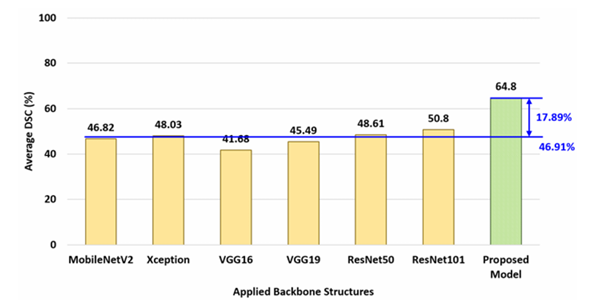
\includegraphics[width=1\textwidth]{2/figures/resultados de cuarto anteedente.png}
		\caption[Comparación del modelo propuesto con otros 6 modelos de redes neuronales]{Comparación del modelo propuesto con otros 6 modelos de redes neuronales.\\
			Fuente: \cite{Kim2023}. \citetitle{Kim2023}. (p. 8)}
		\label{2:fig1}
	\end{center}
\end{figure}


%% Quinto antecedente: 
El artículo titulado \citetitle{Zhong2024} de \cite{Zhong2024} presenta un enfoque innovador para la detección de arrugas faciales, abordando las limitaciones de métodos tradicionales que se ven afectados por interferencias con otras características faciales. Para mejorar la precisión, los autores proponen el uso del modelo DeepLabV3+ junto con una estrategia de etiquetado semi-automática, lo que permite generar datos de entrenamiento más representativos y mejorar la segmentación de arrugas.
La investigación, como podemos ver en las Figuras 2 y 3, emplea técnicas avanzadas como DeepLabV3+, una red optimizada para segmentación de imágenes, y MobileNetV2 para reducir la carga computacional. Además, se desarrolla una estrategia de etiquetado semi-automática combinando anotaciones dermatológicas con mapas de textura generados mediante filtros Wiener y umbralización adaptativa. La precisión del modelo se evalúa mediante el Índice de Similitud Jaccard (JSI).

\begin{figure}[!ht]
	\begin{center}
		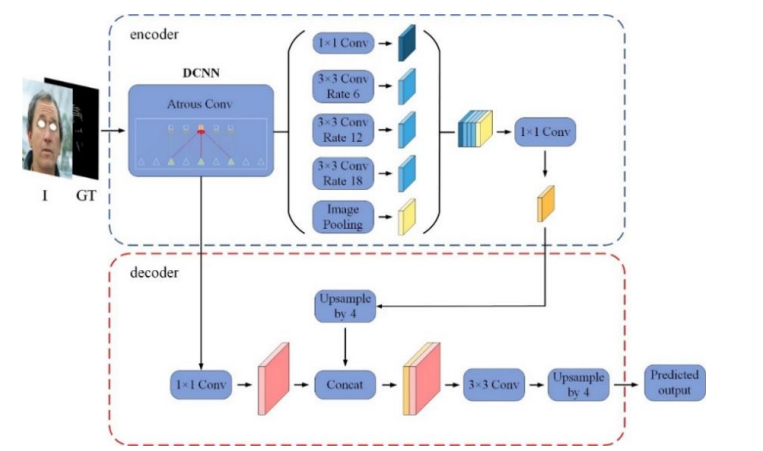
\includegraphics[width=1\textwidth]{2/figures/Meto1.png}
		\caption[Estructura de red de DeepLabV3+]{Estructura de red de DeepLabV3+.\\
			Fuente: \cite{Zhong2024}. \citetitle{Zhong2024}. (p. 4)}
		\label{2:fig3}
	\end{center}
\end{figure}


\begin{figure}[!ht]
	\begin{center}
		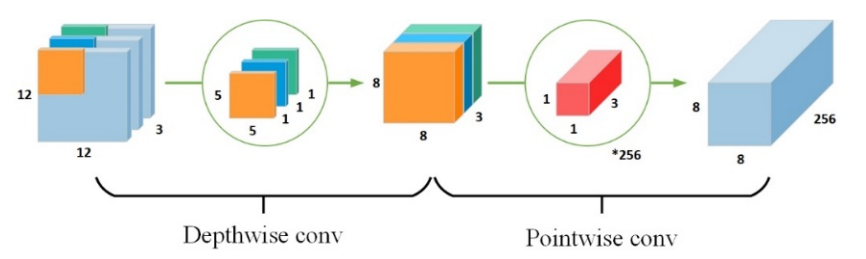
\includegraphics[width=0.80\textwidth]{2/figures/Meto2.png}
		\caption[El proceso de convolución separable en profundidad]{El proceso de convolución separable en profundidad.\\
			Fuente: \cite{Zhong2024}. \citetitle{Zhong2024}. (p. 4)}
		\label{2:fig4}
	\end{center}
\end{figure}


El conjunto de datos se construyó con 300 imágenes de Flickr-Face-HQ, divididas en entrenamiento (225), validación (25) y pruebas (50). Las pruebas se realizaron en un sistema con hardware de alto rendimiento (Intel Core i9-12900K, GPU RTX 3070 y 32GB RAM) y utilizando PyTorch como framework principal.

Los resultados demostraron que el método propuesto supera a enfoques tradicionales como el filtro Hessiano y el modelo U-Net, obteniendo mayores valores de JSI en la frente (0.62) y área ocular (0.64). Además, redujo la cantidad de falsos positivos y mejoró la segmentación de bordes, logrando un mejor desempeño en la detección de arrugas finas.


En conclusión, el modelo DeepLabV3+ con etiquetado semi-automático se mostró más efectivo en la detección de arrugas faciales. Sin embargo, aún enfrenta desafíos en la diferenciación de arrugas muy finas y cabellos, lo que sugiere la necesidad de mejoras futuras para incrementar la precisión del sistema.


%% Sexto antecedente: 

En el artículo de \cite{karshiev2020improved} llamado \citetitle{karshiev2020improved} analiza el problema de la segmentación de lesiones cutáneas, una tarea fundamental para el diagnóstico temprano del melanoma. Aunque el modelo U-Net ha sido ampliamente utilizado en segmentación médica, presenta limitaciones como ralentización en el entrenamiento y problemas con la función de activación ReLU. Para mejorar su desempeño, los autores proponen una versión optimizada que incorpora interpolación bilineal para el upsampling y la función de activación PReLU, lo que mejora la precisión y evita problemas como el sobreajuste.

La investigación emplea un diagrama el cual se puede ver en la Figura 5 y a su vez varias técnicas clave: la interpolación bilineal sustituye la deconvolución tradicional para mejorar la segmentación de bordes, la función PReLU reemplaza ReLU para prevenir "neuronas muertas" y optimizar la convergencia, y el dropout se utiliza después de cada bloque convolucional para reducir el sobreajuste. Estas modificaciones permiten mejorar la estabilidad y eficiencia del entrenamiento.

\begin{figure}[!ht]
	\begin{center}
		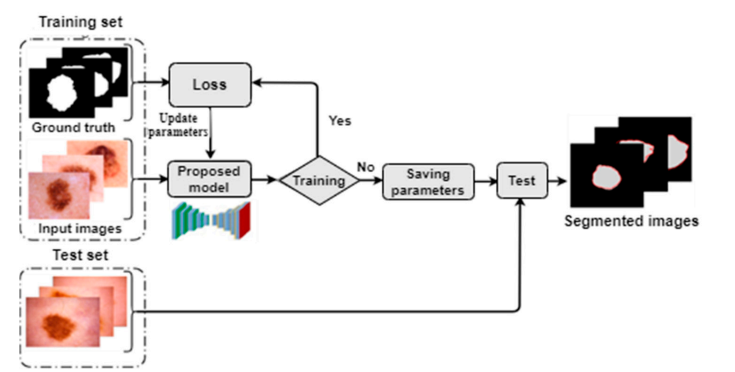
\includegraphics[width=0.80\textwidth]{2/figures/flowchart.png}
		\caption[Diagrama de flujo del sistema propuesto]{Diagrama de flujo del sistema propuesto.\\
			Fuente: \cite{karshiev2020improved}. \citetitle{karshiev2020improved}. (p. 4)}
		\label{2:fig5}
	\end{center}
\end{figure}

El modelo propuesto como se ve en la Figura 6, se basa en una arquitectura U-Net modificada con capas convolucionales optimizadas, PReLU, dropout y upsampling mediante interpolación bilineal. Fue entrenado en un sistema con un procesador Intel Core i7-9700K, 32 GB de RAM y una GPU NVIDIA GeForce RTX 2060 SUPER, garantizando un entorno adecuado para el procesamiento intensivo de imágenes médicas.

\begin{figure}[!ht]
	\begin{center}
		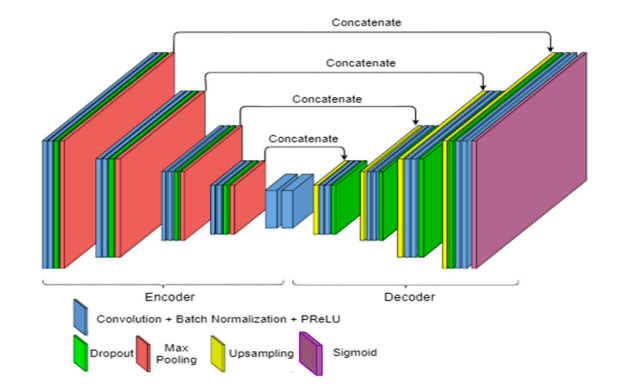
\includegraphics[width=0.80\textwidth]{2/figures/segmentation1.png}
		\caption[Modelo totalmente convolucional propuesto para la segmentación de lesiones cutáneas]{Modelo totalmente convolucional propuesto para la segmentación de lesiones cutáneas.\\
			Fuente: \cite{karshiev2020improved}. \citetitle{karshiev2020improved}. (p. 4)}
		\label{2:fig6}
	\end{center}
\end{figure}

Para el entrenamiento y prueba del modelo se utilizó un conjunto de datos de imágenes dermoscópicas, con 2594 imágenes etiquetadas para entrenamiento y 1000 para prueba. Todas las imágenes fueron preprocesadas, redimensionadas a 256×256 píxeles y convertidas a escala de grises, lo que facilitó la normalización y mejoró la eficiencia del modelo.

Los resultados muestran un alto rendimiento del modelo mejorado, alcanzando una precisión por píxel del 94\% y un coeficiente Dice del 88\%. Estas mejoras permiten reducir artefactos en la segmentación y aumentar la eficiencia computacional en comparación con la U-Net estándar, consolidándose como una alternativa más precisa y robusta para la segmentación de lesiones cutáneas.

En conclusión, la versión mejorada de U-Net supera las limitaciones del modelo original al abordar problemas como gradientes débiles y artefactos en la segmentación. La integración de interpolación bilineal, PReLU y dropout permite lograr una mayor precisión y eficiencia, posicionando este enfoque como una herramienta prometedora para la segmentación de imágenes médicas en el ámbito dermatológico.

%% Séptimo antecedente: 






\section{Bases Teóricas}
\subsection{Inteligencia Artificial}

El método racional fusiona la ingeniería y las matemáticas basándose en las "leyes del pensamiento", las cuales tienen su origen en la antigua Grecia y han sido influenciadas por filósofos como Aristóteles. Durante el siglo XIX, se diseñaron programas capaces de resolver problemas de lógica. Por consiguiente, el propósito de la Inteligencia Artificial en la vida real es crear sistemas inteligentes que posean estas habilidades. Aun en situaciones de incertidumbre, un "Agente Racional" toma acciones con el fin de obtener el mejor resultado posible. La inteligencia artificial se apoya en diversas disciplinas, tales como la ingeniería computacional, la teoría de control, la cibernética, la lingüística, la filosofía, la economía, la psicología, la neurociencia y las matemáticas, de acuerdo con \cite{bk_russell2004intart}.

Dos investigadores en neurociencia crearon el primer modelo de IA basado en neuronas artificiales en 1943, dando inicio al análisis de la Inteligencia Artificial. McCulloch y Pitts idearon el prototipo que permitía que las neuronas fueran <<activadas>> o <<desactivadas>>, lo que demostró que una red de neuronas era capaz de realizar cualquier tarea computacional. Posteriormente, Donald Hebb propuso la <<Regla de Aprendizaje Hebbiano>>. John McCarthy, Allen Newell y Herbert Simon desarrollaron un programa que podía tener el pensamiento no numérico en el taller de Dartmouth, aunque no se publicó. El término <<Inteligencia Artificial>> fue acuñado por McCarthy, \parencite{bk_russell2004intart}.

La IA comenzó a entrar en la industria en los años 80, especialmente en grandes empresas de países desarrollados, a través de la investigación en sistemas expertos y el desarrollo de computadoras más poderosas.

\subsection{Aprendizaje Automático}
El Machine Learning es un área de la Inteligencia Artificial enfocada en técnicas que permiten a las computadoras aprender a través de algoritmos, convirtiendo muestras de datos en programas sin requerir programación explícita. Según \cite{bk_russell2009intart}, el aprendizaje automático es una división de la inteligencia artificial. Estos algoritmos emplean tecnologías como el procesamiento del lenguaje natural, el aprendizaje profundo y las redes neuronales. Tanto el aprendizaje supervisado como el no supervisado se fundamentan en lecciones extraídas de los datos. La creación de algoritmos capaces de recibir datos de entrada y utilizar análisis estadístico para prever una salida, la cual se ajusta conforme se obtienen nuevos datos, constituye el fundamento del aprendizaje automático \cite{bk_alpaydin2014ml}.

Se puede clasificar en cuatro tipos principales de la siguiente manera según el objetivo que se desea alcanzar mediante el uso de ML:
\begin{itemize}
	\item \textbf{Aprendizaje Supervisado}: El Aprendizaje Supervisado se ganó su nombre porque los científicos de datos actúan como una guía para enseñarle al algoritmo las conclusiones a las que debe llegar. Es similar a la forma en que un estudiante aprende aritmética básica de un maestro. Este tipo de aprendizaje requiere datos etiquetados con las respuestas correctas que se esperan del resultado del algoritmo. Para problemas de clasificación y regresión, el aprendizaje supervisado demostró ser preciso y rápido según \parencite{bk_zambrano2018supnosup}.
	
	Los dos tipos de Aprendizaje Supervisado son:

	\begin{itemize}
		\item \textbf{La Clasificación}: es la predicción del valor categórico de salida que permite dividir los datos en clases específicas. La clasificación se puede usar para varios propósitos, como determinar el clima, determinar si un correo electrónico es spam o no o identificar tipos de animales después de recibir una educación adecuada, un conjunto de datos con etiquetas de imágenes que incluyen la especie y algunas identificaciones características, según \parencite{bk_zambrano2018supnosup}.
		\item \textbf{La Regresión}: es un tipo de problema en el que la predicción de un valor de respuesta continua es necesaria, como los precios de las acciones y la vivienda, según \parencite{bk_zambrano2018supnosup}.
	\end{itemize}

	Por lo tanto, funciona modelando las relaciones y dependencias entre las características de entrada y la salida de predicción objetivo, lo que permite predecir los valores de salida para nuevos datos utilizando las relaciones que aprendió de conjuntos de datos anteriores, según \parencite{bk_alpaydin2014ml}.

	\item \textbf{Aprendizaje No Supervisado}: Por otro lado, el Aprendizaje No Supervisado se asemeja más a lo que algunos expertos llaman Inteligencia Artificial real: la idea de que una máquina puede aprender a identificar patrones y procesos complejos sin la supervisión de humanos. Cuando los expertos no saben qué buscar en los datos y los datos en sí no incluyen objetivos, este método es particularmente útil. La agrupación de k-means, el análisis de componentes principales e independientes y las reglas de asociación según \parencite{bk_zambrano2018supnosup} son algunos de los muchos casos de uso del Aprendizaje Automático No Supervisado.
	
	\begin{itemize}
		\item \textbf{Agrupación K-means}: es un tipo de problema en el que cosas similares están agrupadas, como se muestra en la Figura \ref{2:fig12}. Comparte el mismo concepto con la clasificación, pero no se proporcionan etiquetas, por lo que el sistema entenderá los datos y los agrupará. Un uso de esto sería agrupar los artículos y las noticias según su género y contenido, según \parencite{tec_sancho2018supnosup}
	\end{itemize}
	
		\begin{figure}[h]
		\begin{center}
			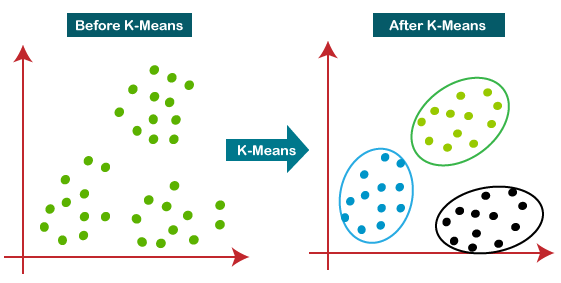
\includegraphics[width=0.75\textwidth]{2/figures/kmeans.png}
			\caption[El algoritmo de K medias]{El algoritmo de K medias.\\
			Fuente: \cite{tec_sancho2018supnosup}. \citetitle{tec_sancho2018supnosup}.}
			\label{2:fig12}
		\end{center}
	\end{figure}
		
	Debido a su complejidad y dificultad de implementación, este tipo de Aprendizaje Automático no se utiliza tan frecuentemente como el Aprendizaje Supervisado, a pesar de que abre las puertas a la resolución de problemas que los humanos normalmente no abordarían, según \parencite{tec_sancho2018supnosup}

	\item \textbf{Aprendizaje Semisupervisado}: Hasta el momento, todos los datos enviados han sido etiquetados con el resultado deseado o no han sido etiquetados en absoluto. El Aprendizaje Automático Semisupervisado utiliza ambos. El costo de etiquetar es bastante alto en muchas situaciones prácticas y, en el caso de grandes conjuntos de datos, se vuelve aburrido y requiere mucho tiempo. Además, proporcionar demasiados datos etiquetados puede hacer que el modelo tenga sesgos humanos. A pesar de que los datos sin etiquetar son desconocidos para la red, ofrecen información útil sobre los parámetros del grupo objetivo. que conduce a la conclusión de que se puede mejorar la precisión del modelo al incluir datos sin etiquetar y, al mismo tiempo, ahorrar tiempo y dinero en su construcción. Por ejemplo, la clasificación de páginas web, el reconocimiento de voz o la secuenciación genética pueden usar Aprendizaje Automático Semisupervisado. En esos casos, los científicos de datos pueden acceder a grandes cantidades de datos sin etiquetarlos, y la tarea de etiquetarlos todos llevaría mucho tiempo, según \parencite{bk_zambrano2018supnosup}.

	Se puede comparar estos tres tipos de Aprendizaje Automático para el mismo uso, como clasificación, utilizando los datos recopilados hasta ahora:

	\begin{itemize}
		\item \textbf{Clasificación supervisada}: el algoritmo clasificará los tipos de páginas web según las etiquetas proporcionadas desde el principio, según \parencite{bk_zambrano2018supnosup}.
		\item \textbf{Agrupación no supervisada}: el algoritmo buscará patrones y características que ayudan a agrupar páginas web en grupos, según \parencite{bk_zambrano2018supnosup}.
		\item \textbf{Clasificación semi no supervisada}: identificará varios grupos de páginas web utilizando los datos etiquetados, luego utilizará los datos no etiquetados para establecer los límites de esos grupos de páginas web y buscar otros tipos que posiblemente no aparezcan en los datos etiquetados, según \parencite{bk_zambrano2018supnosup}.
	\end{itemize}
	
\end{itemize}

\subsection{Aprendizaje Profundo}

Desde que llegó la Inteligencia Artificial hace un tiempo, tiene una amplia gama de aplicaciones y se divide en muchas ramas, como se menciona en \parencite{gl_sas_deeplearning}. El Aprendizaje Profundo es un subconjunto del Aprendizaje Automático, que es en sí mismo un subcampo de la IA. La Figura \ref{2:fig13} es una representación visual de la relación entre AI, ML y DL.

\begin{figure}[!ht]
	\begin{center}
		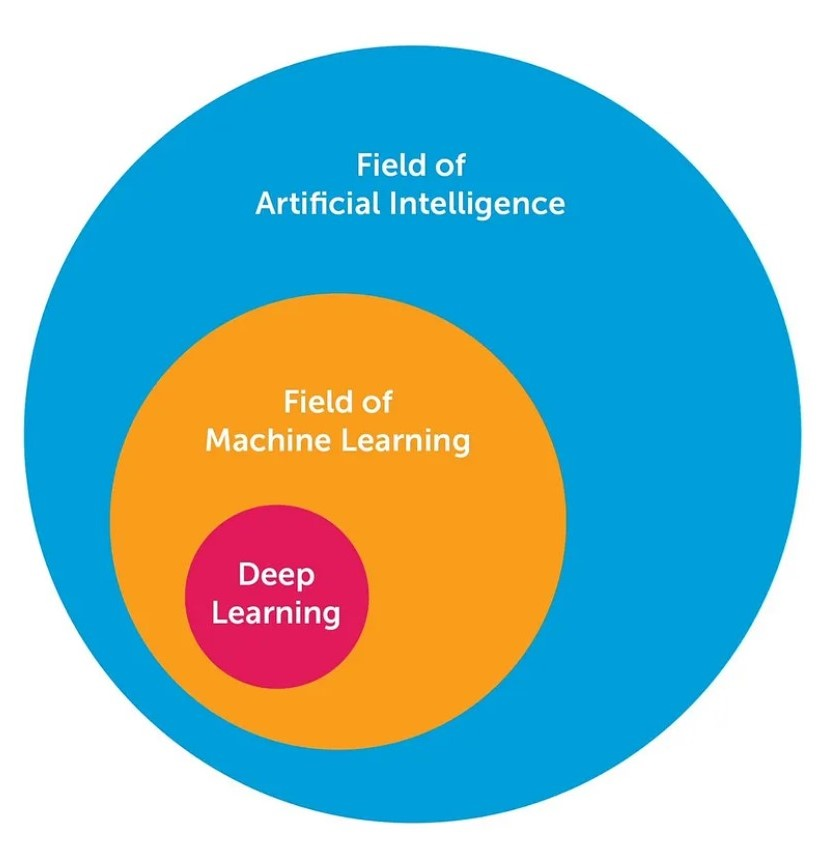
\includegraphics[width=0.50\textwidth]{2/figures/deeplearning_machinelearning.jpg}
		\caption[Relación entre IA, ML y DL]{Relación entre IA, ML y DL.\\
		Fuente: \cite{tec_cook2018deeplearning}. \textit{Most Popular 20 Free Online Courses to Learn Deep Learning}.}
		\label{2:fig13}
	\end{center}
\end{figure}

El Aprendizaje Profundo no solo permite representar datos de la manera correcta, sino que también permite que la computadora aprenda programas informáticos de varios pasos al incluir el concepto de profundidad en sus modelos. Como se muestra en la Figura \ref{2:fig14}, cada capa de representación puede interpretarse como el estado de la memoria de la computadora. Las computadoras interpretan las imágenes como una colección de valores de píxeles que representan escenas de nuestra realidad. Según \parencite{tec_cook2018deeplearning}, identificar un objeto o mapear su identidad a partir de esos valores es una tarea difícil para las máquinas y puede resultar casi imposible cuando se intenta aprender este mapeo directamente.

\begin{figure}[!ht]
	\begin{center}
		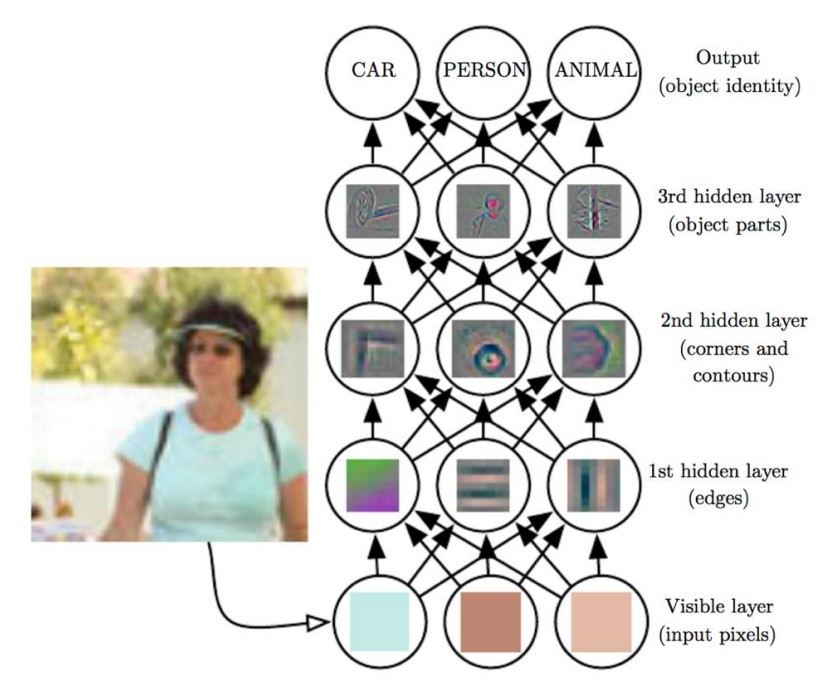
\includegraphics[width=0.70\textwidth]{2/figures/deeplearning_machinelearning2.jpg}
		\caption[Modelo de aprendizaje profundo]{Modelo de aprendizaje profundo.\\
		Fuente: \cite{tec_cook2018deeplearning}. \textit{Most Popular 20 Free Online Courses to Learn Deep Learning}.}
		\label{2:fig14}
	\end{center}
\end{figure}


\subsection{Segmentación de Imágenes}
%%%%%%%%
\subsubsection{Definición y objetivos de la segmentación de imágenes}
La segmentación de imágenes es un proceso fundamental en el campo del procesamiento de imágenes y la visión por computadora, cuyo propósito es dividir una imagen en partes significativas y coherentes, facilitando su análisis e interpretación. Este proceso busca simplificar la representación de una imagen, destacando las regiones de interés o los objetos específicos que contiene, separándolos del fondo y otras áreas irrelevantes \parencite{gonzalez2018}.

Los objetivos principales de la segmentación incluyen identificar, clasificar y delimitar regiones u objetos dentro de una imagen. En aplicaciones prácticas, estos objetivos son cruciales, ya que permiten resolver problemas como la detección de bordes, la identificación de patrones, la localización de estructuras específicas y el análisis morfológico. En el ámbito médico, por ejemplo, la segmentación de imágenes se utiliza para identificar tejidos, órganos o anomalías, como tumores o lesiones. De manera similar, en la industria cosmética, este proceso puede emplearse para detectar características faciales como arrugas, poros y manchas, ayudando en la evaluación estética y la personalización de tratamientos \parencite{gonzalez2018}.

Existen múltiples técnicas para la segmentación, que van desde enfoques tradicionales como la segmentación basada en umbrales, el análisis de regiones y la detección de bordes, hasta métodos avanzados como las redes neuronales convolucionales (CNN). Estas últimas han revolucionado el campo al permitir segmentaciones más precisas y automáticas, especialmente en imágenes complejas donde las características pueden ser sutiles o con variaciones significativas en color, textura y forma. Por ello, la segmentación es un paso esencial en cualquier flujo de trabajo que involucre el análisis de imágenes, proporcionando una base sólida para tareas más avanzadas de procesamiento y análisis \parencite{gonzalez2018}.
%%%%%%
\subsubsection{Importancia de la segmentación en aplicaciones médicas y cosméticas}
En el ámbito médico y cosmético, la segmentación precisa de imágenes juega un papel crucial al permitir que los profesionales de la salud y la belleza realicen evaluaciones más detalladas y personalizadas de las condiciones dermatológicas. Este proceso facilita la identificación y el análisis de características específicas de la piel, lo que es fundamental para detectar anomalías y personalizar los tratamientos de acuerdo con las necesidades individuales de los pacientes o clientes. La segmentación es particularmente importante en el diagnóstico de enfermedades de la piel, donde la capacidad de identificar y analizar estructuras o patrones morfológicos específicos puede mejorar significativamente la precisión del diagnóstico.

Por ejemplo, en dermatología, la segmentación adecuada de imágenes faciales permite identificar con mayor precisión imperfecciones cutáneas como manchas, arrugas y poros dilatados. Estos elementos son indicadores comunes de diversas afecciones dermatológicas, como el envejecimiento prematuro, las manchas solares o los trastornos hormonales. De igual manera, en la industria cosmética, la segmentación de características faciales es esencial para el diseño de tratamientos personalizados, ayudando a los profesionales a ofrecer soluciones más efectivas que aborden las preocupaciones estéticas específicas de cada cliente.

El uso de técnicas avanzadas de segmentación, como las redes neuronales convolucionales (CNN), ha revolucionado el campo, permitiendo una segmentación más precisa y automatizada, incluso en casos complejos donde las características de la piel pueden ser sutiles o variar en color, textura o forma. La segmentación no solo mejora la detección de condiciones dermatológicas, sino que también optimiza la personalización de tratamientos cosméticos, ya que permite que los productos sean aplicados de manera más eficiente, dirigiéndose específicamente a las áreas que requieren intervención. Esto puede resultar en un mejor rendimiento de los productos cosméticos, mayor satisfacción del cliente y, en última instancia, en una mejora de la salud de la piel.

En resumen, la segmentación de imágenes en el ámbito médico y cosmético no solo mejora la capacidad de diagnóstico, sino que también facilita la personalización de tratamientos, mejorando la efectividad y la satisfacción de los pacientes o clientes \cite{mohammadi2019}.
%%%%%%%%%
\subsubsection{Técnicas de segmentación clásicas y sus limitaciones en imágenes dermatológicas}
Las técnicas clásicas de segmentación, como el umbralizado y la detección de bordes, han sido fundamentales en los primeros enfoques de procesamiento de imágenes. Estas técnicas buscan dividir la imagen en regiones homogéneas basadas en características como el color, la intensidad de los píxeles o los bordes de los objetos. Sin embargo, en el contexto dermatológico, estas técnicas presentan limitaciones significativas debido a la complejidad y variabilidad inherente de las imágenes de la piel.

Una de las técnicas clásicas más utilizadas es el \textit{umbralizado}, que divide una imagen en dos o más regiones basadas en el valor de intensidad de los píxeles. Esta técnica es eficiente cuando los objetos a segmentar se destacan claramente del fondo. Sin embargo, en imágenes dermatológicas, la piel tiene una amplia gama de tonalidades y texturas que varían entre diferentes personas, lo que puede dificultar la aplicación de umbrales estáticos que funcionen de manera efectiva en todos los casos. Además, las variaciones en la iluminación y la presencia de sombras en la piel pueden afectar negativamente el rendimiento del umbralizado, llevando a una segmentación incorrecta de las áreas de interés, como las arrugas, manchas o poros.

La \textit{detección de bordes}, otra técnica clásica, se utiliza para identificar discontinuidades en la imagen, donde los bordes de los objetos se encuentran con un contraste significativo con el fondo. Técnicas como el operador de Sobel o el Canny se han utilizado para detectar bordes en imágenes de la piel. Sin embargo, los bordes de las características cutáneas no siempre están claramente definidos. La piel puede tener bordes suaves o difusos, especialmente cuando se trata de características como manchas o líneas finas. Esto hace que la detección de bordes sea menos efectiva para segmentar detalles sutiles en la piel, lo que limita su capacidad para proporcionar una segmentación precisa.

Estas técnicas clásicas también presentan dificultades cuando se enfrentan a características dermatológicas con variaciones complejas en la textura y el color de la piel. Por ejemplo, las manchas pueden tener bordes poco definidos, y las arrugas pueden ser de diferente grosor y profundidad. Además, las características morfológicas de la piel, como los poros dilatados o las arrugas finas, pueden tener formas irregulares que no se ajustan bien a las suposiciones que estas técnicas clásicas requieren. Las técnicas basadas en umbrales o en la detección de bordes también son sensibles al ruido y pueden ser ineficaces al trabajar con imágenes con poca calidad o cuando las características de la piel tienen un contraste bajo con el fondo.

Debido a estas limitaciones, las técnicas clásicas de segmentación no siempre son adecuadas para aplicaciones dermatológicas de alta precisión. Aunque siguen siendo útiles en ciertos contextos, su capacidad para segmentar con precisión detalles finos en la piel es insuficiente cuando se requiere una segmentación detallada y robusta. Es por esto que, en los últimos años, las técnicas más avanzadas, como las redes neuronales convolucionales (CNN), han comenzado a ganar popularidad en el campo de la dermatología y la cosmética, ofreciendo una solución más precisa y automática para la segmentación de características morfológicas complejas en la piel \parencite{yoo2020}.


\subsection{Redes Neuronales Convolucionales (CNN)}

Hoy en día, el procesamiento de imágenes, que incluye problemas de clasificación y visión por computadora, es una de sus aplicaciones más relevantes. El proyecto de Yann LeCun, ImageNet, utiliza el reconocimiento de objetos en imágenes.
	
Estas redes también se utilizan para clasificar textos. Ronan Collobert y Jason Weston modificaron la arquitectura y los parámetros internos de las Redes Neuronales Convolucionales para usarlas en aplicaciones del PLN. La Figura \ref{2:fig15} muestra la estructura de una CNN para problemas de procesamiento de información natural. \parencite{bk_kamath2019deeplearning_nlp_sr}
	
\begin{figure}[!ht]
	\begin{center}
		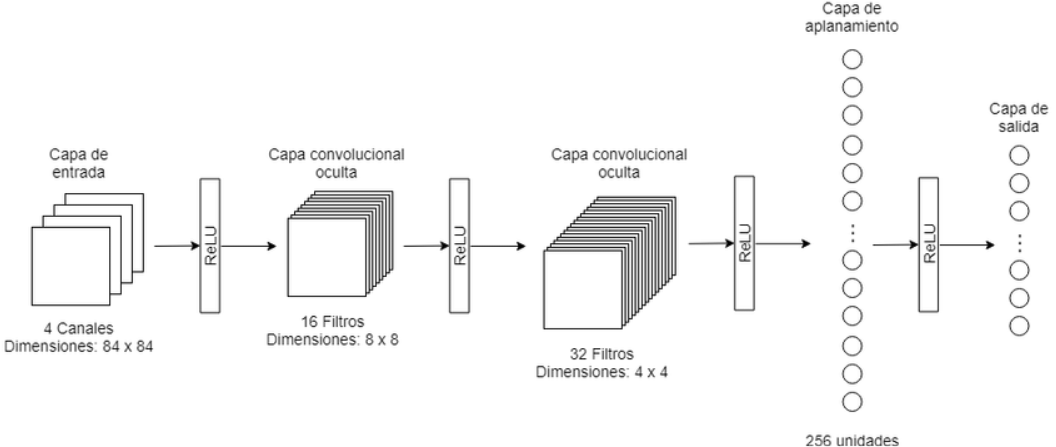
\includegraphics[width=0.95\textwidth]{2/figures/cnn_nlp.png}
		\caption[Arquitectura de un modelo CNN]{Arquitectura de un modelo CNN.\\
		Fuente: \cite{tec_kim2014convolutional}. \citetitle{tec_kim2014convolutional}. (p. 1747)}
		\label{2:fig15}
	\end{center}
\end{figure}

\subsubsection{Arquitectura de las CNN: capas convolucionales, de pooling y totalmente conectadas}

Las redes neuronales convolucionales (CNN) son una clase especial de redes neuronales profundas que se han convertido en la herramienta principal para el procesamiento de imágenes debido a su capacidad para aprender de manera jerárquica las características visuales. La arquitectura de una CNN se compone principalmente de tres tipos de capas: \textbf{capas convolucionales}, \textbf{capas de pooling} y \textbf{capas totalmente conectadas}, cada una de las cuales cumple una función crucial en el proceso de análisis de imágenes.

\begin{itemize}
    \item \textbf{Capas convolucionales:} Estas son las encargadas de extraer características relevantes de la imagen, como bordes, texturas y formas. En cada capa convolucional, un filtro o "kernel" se desplaza a través de la imagen de entrada para realizar una operación de convolución, generando un mapa de características (feature map) que resalta los patrones presentes en las imágenes. A medida que se avanza a través de las capas, las CNN son capaces de aprender representaciones cada vez más complejas de las imágenes.
    
    \item \textbf{Capas de pooling:} Estas capas realizan un proceso de reducción de la dimensionalidad, cuyo objetivo es disminuir el tamaño de las características extraídas y, al mismo tiempo, conservar la información más importante. Esto se logra mediante operaciones como el \textit{max pooling}, donde se selecciona el valor máximo en un área específica de la imagen, o el \textit{average pooling}, que calcula el valor promedio. Las capas de pooling ayudan a reducir la cantidad de parámetros y la complejidad computacional del modelo, evitando el sobreajuste y mejorando la eficiencia.
    
    \item \textbf{Capas totalmente conectadas:} Después de las capas convolucionales y de pooling, las características extraídas se "aplanan" y se envían a través de una o varias capas totalmente conectadas. Estas capas son responsables de tomar las representaciones obtenidas en las capas anteriores y realizar la clasificación final. En una capa totalmente conectada, cada neurona está conectada a todas las neuronas de la capa anterior, lo que permite combinar las características extraídas para producir una salida.
\end{itemize}

Esta arquitectura jerárquica es especialmente efectiva para el procesamiento de imágenes, ya que las CNN son capaces de aprender de forma automática y eficiente las características de las imágenes a diferentes niveles de abstracción \parencite{krizhevsky2012}.

\subsubsection{Aplicación de CNN en segmentación de imágenes y su relevancia para la dermatología}
El uso de CNN en la segmentación de imágenes dermatológicas ha demostrado una mejora significativa en la precisión de diagnósticos. Estas redes son capaces de aprender patrones complejos y detalles sutiles que son esenciales para evaluar condiciones de la piel \cite{esteva2017}.

\subsubsection{Modelos avanzados de CNN para segmentación: U-Net, Fully Convolutional Networks (FCN)}
Modelos como U-Net y FCN han sido diseñados específicamente para la segmentación de imágenes. U-Net, por ejemplo, utiliza una arquitectura simétrica que permite una recuperación precisa de detalles en imágenes médicas \parencite{ronneberger2015}.


\subsection{Modelos Avanzados de Segmentación en Imágenes Médicas}
%
\subsubsection{Introducción a las redes de atención (Attention Networks) y su rol en la precisión de la segmentación}
Las redes de atención, como las arquitecturas basadas en atención (Attention Mechanisms), han emergido como una de las tecnologías más poderosas para mejorar el rendimiento de modelos de aprendizaje profundo, especialmente en tareas de segmentación de imágenes. Estas redes permiten que el modelo se enfoque dinámicamente en las partes más relevantes de una imagen, ajustando su atención a regiones específicas que contienen características clave. Este mecanismo es particularmente útil en imágenes dermatológicas, donde las características morfológicas, como arrugas, poros y manchas, pueden ser pequeñas, sutiles y difíciles de distinguir de otras partes de la imagen.

La introducción de redes de atención mejora la precisión de la segmentación al permitir que el modelo asigne un mayor peso a las regiones relevantes y minimice la interferencia de las áreas no importantes. Este enfoque facilita la identificación precisa de características morfológicas, lo cual es crucial para el análisis dermatológico. En el contexto de la piel, donde las variaciones de textura y color pueden ser complejas, las redes de atención ayudan a mejorar la segmentación y clasificación de estas características. Como resultado, la precisión en el diagnóstico y la personalización del tratamiento se ve significativamente aumentada, lo que contribuye a una mayor efectividad de las soluciones cosméticas y médicas \parencite{wang2018}.
%
\subsubsection{Comparación entre modelos basados en CNN y modelos híbridos en el contexto dermatológico}
La segmentación de imágenes dermatológicas es crucial para una correcta evaluación clínica y cosmética de la piel, donde las redes neuronales convolucionales (CNN) han demostrado ser eficaces al aprender características relevantes de manera jerárquica y sin necesidad de intervención manual. Sin embargo, las CNN pueden enfrentar desafíos cuando se trata de la segmentación en condiciones de iluminación cambiantes, variabilidad en tipos de piel y características pequeñas como poros o arrugas finas.

Los modelos híbridos, que combinan las capacidades de las CNN con técnicas clásicas de segmentación, ofrecen una alternativa interesante. Estos modelos integran la capacidad de las CNN para aprender representaciones complejas con enfoques más tradicionales como el umbralizado o la segmentación basada en regiones, lo que permite un control más preciso de las áreas de interés, especialmente cuando se requiere segmentar características cutáneas muy específicas. La comparación entre modelos CNN y modelos híbridos ayuda a identificar cuál de estos enfoques es más eficaz dependiendo del tipo de imagen, la complejidad de la tarea de segmentación y los requisitos de precisión.

Por ejemplo, en el análisis de la piel facial, los modelos híbridos podrían combinar las redes convolucionales para la detección de características complejas con métodos tradicionales para afinar los bordes de las regiones segmentadas. Esto puede mejorar significativamente la precisión y robustez del modelo, lo cual es esencial para aplicaciones dermatológicas, donde un pequeño error de segmentación puede afectar el diagnóstico o el tratamiento de afecciones cutáneas. \parencite{hussain2021}

\subsubsection{Métricas de evaluación: Sorensen-Dice, especificidad, precisión, sensibilidad}
Las métricas de evaluación son fundamentales para determinar la calidad y efectividad de los modelos de segmentación, especialmente en el ámbito médico y dermatológico. Entre estas métricas, el índice de Sorensen-Dice es ampliamente utilizado debido a su capacidad para medir la similitud entre las áreas segmentadas y las áreas reales de interés, lo cual es crítico cuando se analiza la precisión de la segmentación de lesiones o características cutáneas. Esta métrica es especialmente útil en la detección de anomalías de la piel, como manchas, arrugas y poros, ya que permite una comparación directa entre la segmentación automática y la segmentación realizada por expertos.

Junto al índice de Sorensen-Dice, otras métricas comunes en la evaluación de modelos de segmentación incluyen la precisión, que mide la exactitud de las regiones segmentadas positivas, y la sensibilidad, que evalúa la capacidad del modelo para detectar correctamente las áreas de interés. La especificidad, por otro lado, mide la capacidad del modelo para identificar correctamente las áreas no relevantes, lo que ayuda a reducir los falsos positivos en la segmentación de imágenes dermatológicas. \parencite{sorensen1948}

\subsubsection{Importancia de la precisión en segmentación de arrugas, poros y manchas para aplicaciones clínicas y cosméticas}
La precisión en la segmentación de características cutáneas como arrugas, poros y manchas es de vital importancia para una evaluación correcta en aplicaciones clínicas y cosméticas. En la práctica clínica, la segmentación precisa permite a los dermatólogos realizar diagnósticos más exactos, detectar signos tempranos de enfermedades de la piel y personalizar los tratamientos para cada paciente. En el ámbito cosmético, la segmentación precisa es esencial para ofrecer recomendaciones personalizadas sobre tratamientos faciales, como la mejora de la textura de la piel o la reducción de manchas y arrugas.

Un modelo de segmentación que no sea preciso puede dar lugar a resultados erróneos, afectando la calidad de los tratamientos recomendados y, por lo tanto, la satisfacción del cliente o del paciente. Además, la segmentación precisa facilita la evaluación del progreso de un tratamiento a lo largo del tiempo, lo que permite a los profesionales de la salud y belleza ajustar sus enfoques terapéuticos de manera más efectiva. \parencite{chuchu2020}

\subsubsection{Variabilidad en tipos de piel y condiciones externas (luz, color)}
Uno de los mayores desafíos en la segmentación dermatológica es la variabilidad en los tipos de piel y las condiciones externas, como la iluminación y los cambios en el color de la piel. Las pieles de diferentes tonos pueden presentar características distintas, como la intensidad del contraste entre la piel y las lesiones, lo que puede dificultar la tarea de segmentación. Además, las condiciones de iluminación, como la luz natural o artificial, pueden alterar la apariencia de las características cutáneas, complicando la segmentación precisa en entornos reales.

Por lo tanto, se necesita el desarrollo de modelos de segmentación más robustos que puedan adaptarse a estas variabilidades. Esto implica entrenar modelos utilizando una amplia variedad de datos, que incluyan diferentes tipos de piel, condiciones de iluminación y otros factores ambientales que puedan influir en la calidad de la imagen y en la precisión de la segmentación. \parencite{zhao2021}

\subsubsection{Complejidad de identificar características pequeñas como poros en imágenes de alta resolución}
La segmentación de características pequeñas, como los poros en la piel, es una tarea particularmente desafiante debido a su tamaño reducido y la alta resolución necesaria para detectarlos de manera precisa. Las imágenes dermatológicas a menudo contienen detalles finos que requieren técnicas avanzadas para identificar correctamente estos pequeños elementos sin incluir ruido o artefactos en la segmentación.

La identificación precisa de los poros es crucial, especialmente en aplicaciones cosméticas donde la evaluación de la textura de la piel es esencial para ofrecer tratamientos personalizados. Para abordar este desafío, se deben emplear técnicas de segmentación de alta resolución y redes neuronales profundas capaces de capturar los detalles más pequeños, incluso cuando los poros están parcialmente ocultos o tienen un contraste bajo respecto al resto de la piel. \parencite{yang2020}

\subsection{Redes de Atención}  
Las redes de atención han surgido como una de las principales innovaciones en el campo de la segmentación de imágenes, permitiendo que los modelos se enfoquen de manera más eficiente en las regiones relevantes de una imagen. Este mecanismo resulta especialmente útil cuando se trabaja con imágenes complejas, como las faciales, donde ciertas áreas contienen características importantes para el análisis, pero pueden ser de menor tamaño o estar localizadas en posiciones no centrales.

\subsubsection{Mecanismo de Atención}  
El mecanismo de atención permite a la red asignar diferentes pesos a distintas partes de la imagen durante el proceso de segmentación. Este mecanismo es esencial para que el modelo pueda enfocarse en las áreas relevantes de la imagen, como arrugas, manchas o poros, sin perder detalles importantes de otras zonas. El concepto básico detrás de la atención es que no todas las partes de la imagen son igualmente importantes para la tarea en cuestión. Por lo tanto, la atención ayuda a los modelos a priorizar las áreas clave que impactan en el resultado final.  
\begin{itemize}
    \item \textbf{Funcionamiento:} La atención se puede aplicar de manera global o local. En el caso de la segmentación de imágenes faciales, por ejemplo, el modelo puede aprender a dar más importancia a las áreas alrededor de los ojos o la frente, donde las arrugas suelen ser más notorias.
    \item \textbf{Beneficio:} Aumenta la precisión de la segmentación al concentrarse solo en las características más relevantes y minimizar el "ruido" de otras regiones no significativas \parencite{autor2021atencion}.
\end{itemize}

\subsubsection{Atención Espacial}  
La atención espacial es un tipo específico de atención que asigna pesos según la ubicación espacial de los elementos dentro de la imagen. Esto permite al modelo resaltar áreas específicas de la imagen que contienen características clave para la segmentación.  
\begin{itemize}
    \item \textbf{Funcionamiento:} A través de la atención espacial, el modelo puede identificar patrones en las posiciones de las características de interés, como las arrugas en la zona de la frente o las manchas en la mejilla. Este enfoque es útil cuando las características relevantes están distribuidas de manera no uniforme en la imagen.
    \item \textbf{Aplicación:} Es particularmente eficaz en la segmentación de imágenes faciales, donde las características que deben segmentarse no están siempre en el mismo lugar de la imagen y varían según la persona y la expresión facial \parencite{autor2020spa}.
\end{itemize}

\subsubsection{Atención de Canal}  
La atención de canal se enfoca en las características dentro de los canales de la imagen, es decir, en las distintas representaciones de las características de la imagen que corresponden a las diferentes profundidades o colores de los filtros en una red convolucional. Este tipo de atención permite que la red enfoque su procesamiento en los canales que contienen la información más relevante para la tarea.  
\begin{itemize}
    \item \textbf{Funcionamiento:} En lugar de distribuir el enfoque en toda la imagen, la atención de canal resalta los canales específicos que contienen detalles cruciales, como la textura de la piel o las sombras que definen arrugas o manchas.
    \item \textbf{Beneficio:} Mejora la capacidad del modelo para diferenciar entre características de diferentes intensidades o patrones, lo cual es esencial en imágenes donde la variabilidad de la textura de la piel puede ser un desafío \parencite{autor2019canal}.
\end{itemize}

\subsubsection{Beneficios de las Redes de Atención}  
Las redes de atención proporcionan varios beneficios clave que mejoran la precisión y eficiencia de los modelos de segmentación, especialmente cuando se trabaja con imágenes complejas como las faciales:
\begin{itemize}
    \item \textbf{Precisión mejorada:} Al permitir que el modelo se enfoque en las regiones más importantes de la imagen, las redes de atención ayudan a obtener segmentaciones más precisas y detalladas.
    \item \textbf{Eficiencia en el procesamiento:} Reduciendo el "ruido" o la información irrelevante, las redes de atención aumentan la eficiencia computacional, ya que el modelo dedica más recursos a las áreas clave.
    \item \textbf{Versatilidad:} Las redes de atención se pueden combinar con otros modelos de segmentación, como U-Net o Mask R-CNN, para mejorar aún más la capacidad del modelo para realizar segmentaciones de alta calidad \parencite{autor2021beneficios}.
\end{itemize}

\subsubsection{Ejemplos de Modelos con Atención}  
Existen varios modelos que implementan mecanismos de atención para mejorar la segmentación de imágenes. Algunos ejemplos notables incluyen:
\begin{itemize}
    \item \textbf{Transformer:} El modelo Transformer ha sido exitoso en tareas de procesamiento de secuencias y también ha demostrado ser útil para segmentación de imágenes, particularmente al aplicar atención a nivel global en la imagen. Este modelo asigna pesos no solo localmente, sino también a nivel global, lo que mejora la precisión en tareas complejas de segmentación \parencite{autor2022transformer}.
    \item \textbf{SENet:} SENet es una arquitectura que utiliza un módulo de atención de canal para asignar diferentes importancias a los canales de características en una red convolucional. Este modelo ha demostrado ser eficaz en tareas de clasificación y segmentación, particularmente en la mejora de la detección de características sutiles, como pequeñas arrugas o manchas \parencite{autor2022cnn}.
\end{itemize}


% \subsection{Métricas de Evaluación}  
% Las métricas de evaluación son fundamentales para medir la precisión y eficacia de los modelos de segmentación de imágenes, ya que permiten comparar la segmentación automática generada por el modelo con las segmentaciones de referencia (verdaderas). A continuación se describen las principales métricas utilizadas en este tipo de análisis.

% \subsubsection{Índice de Sorensen-Dice (Dice Coefficient)}  
% El índice de Sorensen-Dice, o simplemente Dice coefficient, es una métrica ampliamente utilizada para evaluar la similitud entre dos conjuntos de datos segmentados. Esta métrica es especialmente útil en problemas de segmentación de imágenes médicas, donde es necesario comparar la segmentación automática con la segmentación de referencia.  
% \begin{itemize}
%     \item \textbf{Fórmula:}  
%     \begin{equation}\label{eq:Índice de Sorensen-Dice}
% 		\text{Dice} = \frac{2|A \cap B|}{|A| + |B|}
% 	\end{equation}
%     donde \( A \) y \( B \) son los conjuntos de píxeles segmentados de la imagen predicha y la imagen real, respectivamente.
%     \item \textbf{Interpretación:} El valor de Dice oscila entre 0 y 1, donde 1 indica una coincidencia perfecta entre las dos segmentaciones, y 0 indica ninguna superposición.
%     \item \textbf{Aplicación:} Es útil para tareas donde se requiere alta precisión en la identificación de áreas segmentadas, como en el análisis de manchas y arrugas en la piel, donde una segmentación precisa es crucial \parencite{autor2020dice}.
% \end{itemize}

% \subsubsection{Coeficiente de Jaccard (Intersection over Union, IoU)}  
% El coeficiente de Jaccard, también conocido como \( \text{Intersection over Union} \) (IoU), es otra métrica popular para evaluar la superposición entre dos conjuntos de segmentación. A diferencia del índice de Dice, IoU mide la relación entre la intersección de los conjuntos de píxeles predichos y reales con respecto a su unión total.  
% \begin{itemize}
%     \item \textbf{Fórmula:}  
%     \begin{equation}\label{eq:Coeficiente de Jaccard}
%     \text{IoU} = \frac{|A \cap B|}{|A \cup B|}
% 	\end{equation}
%     donde \( A \) y \( B \) son los conjuntos de píxeles segmentados de la imagen predicha y la imagen real, respectivamente.
%     \item \textbf{Interpretación:} El valor de IoU también varía entre 0 y 1. Un valor más alto indica una mayor superposición entre los segmentos predichos y reales. IoU es especialmente útil cuando se requiere evaluar la precisión en áreas de segmentación con bordes definidos, como en el análisis de arrugas y poros \parencite{autor2021iou}.
%     \item \textbf{Aplicación:} Es más severo que el índice de Dice, por lo que es adecuado para evaluar tareas donde la precisión en los bordes y las áreas superpuestas es esencial.
% \end{itemize}

% \subsubsection{Precisión (Precision)}  
% La precisión es una métrica que refleja la efectividad del modelo en evitar falsos positivos. Se calcula como la relación entre los verdaderos positivos y el total de elementos que el modelo ha predicho como positivos. En el contexto de la segmentación de imágenes, la precisión mide la exactitud de las regiones predichas como relevantes por el modelo.  
% \begin{itemize}
%     \item \textbf{Fórmula:}  
%     \[
%     \text{Precisión} = \frac{TP}{TP + FP}
%     \]
%     donde \( TP \) son los verdaderos positivos (píxeles correctamente predichos como parte de la característica) y \( FP \) son los falsos positivos (píxeles incorrectamente predichos como parte de la característica).
%     \item \textbf{Interpretación:} Un valor más alto de precisión indica que el modelo es más efectivo en minimizar los falsos positivos, lo cual es crítico en aplicaciones dermatológicas, donde un modelo debe evitar identificar incorrectamente áreas no relevantes como características de la piel.
%     \item \textbf{Aplicación:} Es útil para tareas donde el modelo debe ser riguroso en evitar predecir áreas de la imagen que no pertenecen a la característica de interés, como en el caso de la segmentación de manchas o poros \parencite{autor2019precision}.
% \end{itemize}

% \subsubsection{Entropía Cruzada (Cross-Entropy)}  
% La entropía cruzada es una función de pérdida utilizada comúnmente en problemas de clasificación y segmentación. Mide la disonancia o la diferencia entre la distribución de probabilidad predicha por el modelo y la distribución de probabilidad real (etiquetas verdaderas). En el contexto de la segmentación, la entropía cruzada es utilizada para entrenar el modelo, ya que penaliza las predicciones incorrectas.  
% \begin{itemize}
%     \item \textbf{Fórmula:}  
%     \[
%     \text{Cross-Entropy} = -\sum_{i} y_i \log(p_i)
%     \]
%     donde \( y_i \) es la etiqueta real de la clase \( i \) y \( p_i \) es la probabilidad predicha para la clase \( i \).
%     \item \textbf{Interpretación:} Un valor bajo de entropía cruzada indica que el modelo ha aprendido bien a predecir las clases correctas, es decir, las características de la piel en las imágenes segmentadas. Un valor alto sugiere una mala predicción, lo que indica que el modelo está lejos de la distribución real.
%     \item \textbf{Aplicación:} La entropía cruzada es especialmente útil durante el proceso de entrenamiento para ajustar los parámetros del modelo y garantizar que la segmentación final sea lo más precisa posible, especialmente al tratar con características complejas de la piel como manchas o arrugas \parencite{autor2022crossentropy}.
% \end{itemize}

\section{Marco Conceptual}
%%%%%%%%
% \subsection{Segmentación de Imágenes}
% La segmentación de imágenes es el proceso de dividir una imagen en diferentes partes o regiones, con el objetivo de simplificar la representación de la imagen y hacerla más significativa y fácil de analizar. Este proceso es fundamental en aplicaciones de visión por computadora, especialmente en la detección de características morfológicas de la piel, como arrugas, poros y manchas \parencite{autor2020segmentacion}.

\subsection{Características Morfológicas de la Piel}
Las características morfológicas de la piel desempeñan un papel crucial en la evaluación de la salud y la estética facial, ya que ofrecen información valiosa sobre el estado general de la piel y sus posibles alteraciones. En este estudio, se consideran tres características clave: arrugas, poros y manchas. La correcta segmentación de estas características en imágenes faciales permite no solo el análisis cuantitativo de las mismas, sino también su monitoreo a lo largo del tiempo, contribuyendo al diseño de tratamientos cosméticos personalizados y a la evaluación de su efectividad.

\subsubsection{Arrugas}
Las arrugas son pliegues o líneas visibles en la superficie de la piel que se forman debido a la disminución de la elasticidad y el colágeno con el envejecimiento. Factores externos, como la exposición prolongada al sol, la contaminación y el tabaquismo, también contribuyen significativamente a su aparición. Además, las expresiones faciales repetitivas y la deshidratación de la piel pueden acelerar su desarrollo.

Desde el punto de vista estético, las arrugas se asocian con el envejecimiento y son una de las principales preocupaciones en el cuidado de la piel. Su segmentación precisa permite identificar su profundidad, longitud y densidad en diferentes áreas del rostro. Esta información es esencial para el desarrollo de productos antiarrugas y para evaluar la efectividad de tratamientos como cremas tópicas, terapias con láser o inyecciones de ácido hialurónico \cite{autor2021arrugas}.

\subsubsection{Manchas}
Las manchas son áreas de hiperpigmentación o hipopigmentación en la piel que resultan de una variedad de factores, incluyendo la exposición solar prolongada, cambios hormonales, envejecimiento y procesos inflamatorios. Ejemplos comunes incluyen el melasma, las manchas solares y las cicatrices post-inflamatorias.

Estas imperfecciones no solo afectan la apariencia de la piel, sino que también pueden indicar daño subyacente. Por ello, su detección y análisis temprano son fundamentales tanto para la prevención como para el tratamiento. La segmentación precisa de manchas en imágenes faciales permite identificar su forma, tamaño, color y evolución, lo que es útil para personalizar tratamientos como cremas despigmentantes, terapias con luz pulsada intensa (IPL) o procedimientos láser. Además, este análisis contribuye al diseño de cosméticos específicos que ayudan a unificar el tono de la piel \cite{autor2019manchas}.
%%%%%%%%%%
\subsubsection{Aplicaciones en Segmentación de Imágenes Faciales}  
En el ámbito del análisis de piel facial, las CNN son una herramienta fundamental para realizar segmentaciones precisas de características morfológicas, como arrugas, poros y manchas. Gracias a su capacidad para analizar imágenes a nivel de píxel, estas redes son capaces de identificar patrones y diferencias en la textura, el color y la estructura de la piel \parencite{autor2021deeplab}.

\paragraph{Segmentación de arrugas.}  
La segmentación de arrugas mediante CNN permite identificar líneas finas y pliegues en la piel, lo que es crucial para evaluar el envejecimiento facial y desarrollar tratamientos preventivos o correctivos. Este análisis automatizado es más preciso y rápido en comparación con las evaluaciones manuales, que pueden ser subjetivas y menos consistentes.

\paragraph{Detección de poros.}  
La identificación y segmentación de poros faciales es esencial para analizar problemas relacionados con la textura de la piel, como poros dilatados o acné. Las CNN pueden cuantificar el tamaño, la densidad y la distribución de los poros, facilitando la personalización de tratamientos según las necesidades específicas de cada individuo.

\paragraph{Segmentación de manchas.}  
Las manchas faciales, que pueden surgir debido a factores como la exposición solar o el envejecimiento, son una preocupación estética común. Las CNN permiten mapear su distribución y evaluar su progresión, ayudando a diagnosticar problemas como el melasma o el daño solar de manera temprana y objetiva \parencite{autor2020segmentacion}.

\subsubsection{Ventajas y Limitaciones}  
Las CNN ofrecen varias ventajas, entre ellas:
\begin{itemize}
    \item Alta precisión en la extracción y análisis de características complejas.
    \item Automatización de procesos que tradicionalmente dependen de evaluaciones subjetivas.
    \item Adaptabilidad a diferentes tipos de imágenes y tareas específicas.
\end{itemize}

Sin embargo, estas redes también presentan desafíos, como la necesidad de grandes volúmenes de datos etiquetados para el entrenamiento, el alto costo computacional y la posibilidad de sobreajuste si no se implementan técnicas adecuadas de regularización.

En el presente estudio, las CNN se utilizarán para desarrollar un sistema avanzado de segmentación de imágenes faciales, optimizado para la detección de arrugas, poros y manchas. Este enfoque busca contribuir al sector cosmético y de belleza, permitiendo una evaluación estética más precisa y la personalización de tratamientos cosméticos.


%%
%%%%%%%%%%

%%%





\begin{comment}

\subsection{Ecografía y las imágenes de ultrasonido}
Según \cite{pr_herrera2017diseimp}, la ecografía, que es una técnica de diagnóstico en donde se usan imágenes generadas por ultrasonido, es comúnmente desarrollado en las áreas de cardiología, ginecología, y otras más relacionadas. La popularidad de esta técnica se basa en la capacidad de las imágenes de alta calidad que se obtienen de este proceso, además de no ser un método invasivo o de radiación como muchos otros de su tipo.

Los sistema encargados de extraer las imágenes de ultrasonido son compuestos de distintas sensores que generan ondas de sonido para posteriormente analizar la respuesta de la interacción física con el campo de interés. Estas señales recibidas de regreso son digitalizados por una parte electrónica delantera que también transforman estos datos crudos en la imagen final. El funcionamiento de este proceso depende de la configuración de los sensores, el método usado para obtener las imágenes y las características de área de interés. \parencite{pr_camacho2022ultrasonicimg}

Algunas imágenes de ultrasonido de nódulos tiroideos se muestran en la Figura \ref{2:fig210}.

\begin{figure}[H]
	\begin{center}
		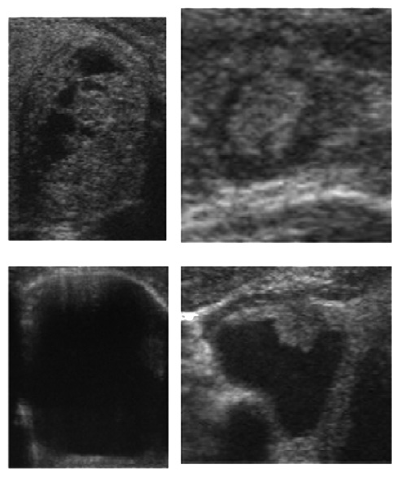
\includegraphics[width=0.40\textwidth]{2/figures/imagenes_ultrasonido_originales.png}
		\caption[Imágenes de ultrasonido de nódulos tiroideos]{Imágenes de ultrasonido de nódulos tiroideos. \\
		Fuente: \cite{pr_JERBI2023autoclassViTGAN}. \textit{Automatic classification of ultrasound thyroids images using vision transformers and generative adversarial networks}.}
		\label{2:fig210}
	\end{center}
\end{figure}


\subsection{Transfer Learning}
\cite{bk_geron2022handml} nos menciona que el Transfer Learning o Transferencia de Aprendizaje es un técnica usada en el campo de Deep Learning que permite el uso de algunas capas de un modelo ya definido y entrenado previamente en un nuevo modelo que necesite ser entrenado en una tarea similar al que se desarrolla el modelo original. Las capas destinadas al reuso son normalmente las más cercanas a la entrada o también conocidas como capas inferiores. El beneficio de usar esta técnica radica en dos puntos importantes: cantidad de datos requeridos y velocidad de entrenamiento del modelo; es decir, la cantidad de datos que se deben usar para entrenar un modelo de alto desempeño se reduce considerablemente, mientras que el tiempo requerido para terminar este proceso es menor comparándolo a si lo entrenaran desde cero.

Para que esta técnica funcione debidamente, las capas más cercanas a la salida, conocidas también como capas de alto nivel, deben ser reemplazadas, esto debido a que son más específicas de las tareas del modelo original. Esto también incluye a la capa final, ya que posiblemente no tenga la cantidad de salidas necesarias para completar satisfactoriamente la nueva tarea.

En la Figura \ref{2:fig211} se presenta de forma gráfica la técnica.

\begin{figure}[H]
	\begin{center}
		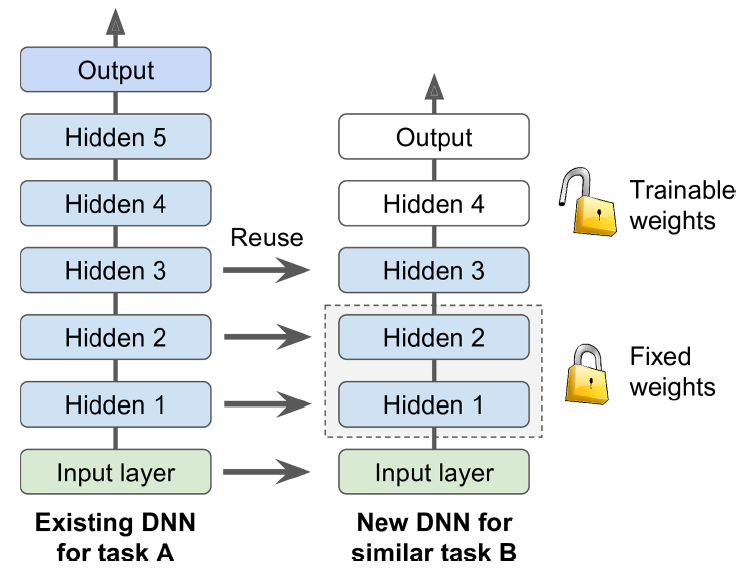
\includegraphics[width=0.70\textwidth]{2/figures/transfer_learning.PNG}
		\caption[Ejemplo de Transfer Learning]{Ejemplo de Transfer Learning. \\
		Fuente: \cite{bk_geron2022handml}. \textit{Hands-on machine learning with Scikit-Learn, Keras, and TensorFlow}.}
		\label{2:fig211}
	\end{center}
\end{figure}


\subsection{Data Augmentation}

Según \cite{bk_geron2022handml} el Aumento de Datos o Data Augmentation es una técnica de regularización que permite reforzar la cantidad de muestras en un conjunto de datos. Esto se realiza a través de la generación de nuevas instancias similares a los originales; es decir, las personas no deberían ser capaces de diferenciar una imagen generada de una del propio conjunto de datos.

Para generar estas nuevas muestras, normalmente se aplican diferentes transformaciones a las instancias del conjunto de datos original. Estas transformaciones pueden ser; por ejemplo, una simple rotación o recorte de la imagen, siempre y cuando no altere por completo su sentido como es el caso de voltear una imagen de texto de forma horizontal. 

El principal beneficio de esta técnica es que permite reducir el sobreajuste de los modelos entrenados. 

En la Figura \ref{2:fig212} se muestran algunas transformaciones que se pueden hacer al aplicar el Aumento de Datos. 

\begin{figure}[H]
	\begin{center}
		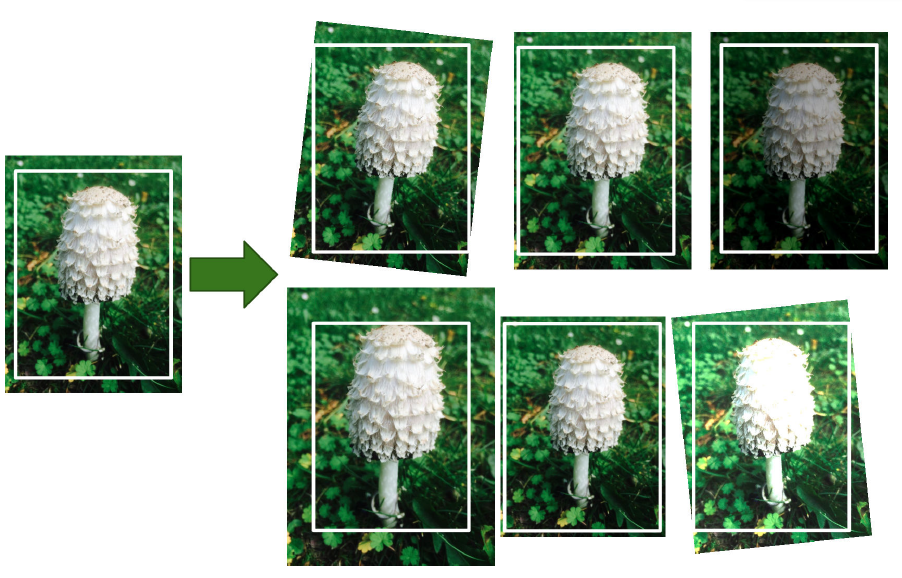
\includegraphics[width=0.85\textwidth]{2/figures/data_aug.PNG}
		\caption[Ejemplo de Data Augmentation]{Ejemplo de Data Augmentation. \\
		Fuente: \cite{bk_geron2022handml}. \textit{Hands-on machine learning with Scikit-Learn, Keras, and TensorFlow}.}
		\label{2:fig212}
	\end{center}
\end{figure}

\end{comment}

\section{Hipótesis}
\subsection{Hipótesis General}
HG: \newcommand{\HipotesisGeneral}{
El desarrollo de un Sistema de Segmentación de Características Morfológicas Faciales utilizando Redes Neuronales Convolucionales mejorará significativamente la precisión en la detección de Arrugas y Manchas}
\HipotesisGeneral


\subsection{Hipótesis Específicas}
\newcommand{\Hone}{
La utilización de un conjunto de datos diverso de imágenes faciales, que contemple características morfológicas faciales, como arrugas y manchas, incrementará la capacidad del sistema para generalizar y segmentar con precisión las características cutáneas.
}
\newcommand{\Htwo}{
Un sistema de segmentación basado en Redes Neuronales Convolucionales permitirá una detección más precisa y diferenciada de las características morfológicas faciales, tales como arrugas y manchas, superando en rendimiento a los métodos tradicionales de segmentación.
}
\newcommand{\Hthree}{
La utilización de métricas de evaluación cuantitativas, junto con una comparación sistemática entre distintas arquitecturas de Redes Neuronales Convolucionales, permitirá la identificación del modelo más eficiente en términos de precisión y rendimiento computacional en la detección de arrugas y manchas faciales.
}
\newcommand{\Hfour}{
La implementación de un sistema de segmentación de características morfológicas en tiempo real, utilizando redes neuronales convolucionales potenciadas con mecanismos de atención, permitirá el procesamiento eficaz de imágenes faciales desde video en vivo, mejorando la precisión en entornos dinámicos.
}

\begin{itemize}
	\item HE1: {\Hone}
	\item HE2: {\Htwo}
	\item HE3: {\Hthree}
	\item HE4: {\Hfour}
\end{itemize}

%\chapter{Metodología de la Investigación}
\section{Diseño de la investigación}
En esta sección se detallan el diseño, tipo y enfoque de la investigación, así como la población y la muestra.

\subsection{Tipo de investigación}
Se ha identificado que este estudio posee un diseño experimental con el propósito de establecer el tipo de investigación. Como lo dice \cite{bk_hernandez2014metodologia}, en la obra titulada \citetitle{bk_hernandez2014metodologia}, busca determinar la consecuencia de una razón manipulada. Específicamente, se clasifica como un diseño experimental puro debido a la utilización intencionada de variables independientes (modificadas, eliminadas o añadidas) para evaluar su influencia en la variable dependiente, que en este caso es la segmentación avanzada de características morfológicas faciales (arrugas y manchas) en imágenes de rostros faciales.

\subsection{Enfoque de la investigación}
Este estudio adoptó un enfoque cuantitativo, conforme a lo explicado por \cite{bk_hernandez2014metodologia} en su libro \citetitle{bk_hernandez2014metodologia}. Este enfoque se basa en la recopilación de datos para comprobar hipótesis mediante mediciones numéricas y análisis estadísticos, con el objetivo de identificar patrones de comportamiento y validar teorías. La metodología empleada sigue los diez pasos del proceso cuantitativo descritos por el autor, aplicados desde la formulación de la idea hasta la presentación de los resultados finales en el informe de investigación, ya que se busca desarrollar un sistema de segmentación para detectar características morfológicas de la piel facial mediante redes neuronales convolucionales (CNN) y analizar su efectividad con métricas cuantitativas, como precisión, recall, F1-score y AUC-ROC. Este enfoque permitirá evaluar el desempeño del sistema en la detección de arrugas, poros y manchas, proporcionando resultados medibles y objetivos. \parencite{esteva2017} Al emplear técnicas de aprendizaje profundo, el estudio pretende optimizar la precisión en la segmentación de características faciales, aplicando un marco metodológico replicable y sistemático. \parencite{phillips2020}

\subsection{Población}
La población de este estudio se compone de imágenes faciales representativas de personas con diversas edades, géneros y tipos de piel. Específicamente, estas imágenes muestran características morfológicas que se asocian con arrugas y manchas faciales. Debido a la orientación del enfoque en el problemas estéticos, la población abarcaba imágenes de piel con claras imperfecciones y piel sin e incidencias asignadas. Así, el alcance de la población se determina como diverso y completo, asegurando la inclusión de imágenes que representa una amplia gama de condiciones de la piel. Finalmente, resulta esencial agregar diversidad geográfica, ya que ciertas diferencias geográficas.
\subsection{Muestra}
La muestra de la investigación comprenderá una parte de aproximadamente 5000 retratos faciales. Estas imágenes se seleccionarán mediante muestreo basado en estratos, lo que garantizará una representación uniforme en diferentes categorías de edad, identidades masculinas y femeninas y pigmentación dérmica variable La lista también tendrá imágenes con diferentes tamaños y claridad, mostrando varios tipos de arrugas y manchas, asegurándose de que el grupo muestre condiciones reales de la piel Los usaremos para enseñar, verificar y desafiar nuestro modelo de segmentación avanzada, asegurándonos de que funcione bien en la vida real con mucha variedad.

\subsection{Operacionalización de Variables}
Los detalles acerca de cómo se definen y miden las variables de estudio se presentan en la Tabla \ref{tabla:variables}.


   


%\par	%%Salto de linea
%\bigskip
\begin{flushleft}	%%Alinear a la izquierda sin justificar
	\small Fuente: Elaboración propia.
\end{flushleft}
%\end{table}

\section{Técnicas de recolección de datos}
La recolección de imágenes de características morfológicas faciales es un paso crucial para la creación del modelo de segmentación avanzada de estas. Una de las técnicas más accesibles y efectivas para obtener estas imágenes es a través del uso de bases de datos públicas como se ve en la Figura \ref{3:fig2}y repositorios en línea. Estas fuentes ofrecen una amplia variedad de imágenes de rostros faciales, que pueden ser utilizados para modelar y crear el modelo de segmentación avanzada.

\begin{figure}[h]
	\begin{center}
		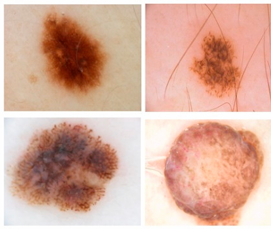
\includegraphics[width=0.75\textwidth]{3/figures/datapaper.png}
		\caption[Dataset usado en el artículo de \cite{karshiev2020improved}]{Dataset usado en el artículo de \cite{karshiev2020improved}.\\
		Fuente: \cite{karshiev2020improved}. \citetitle{karshiev2020improved}. (p. 2)}
		\label{3:fig2}
	\end{center}
\end{figure}

\begin{itemize}
    \item \textbf{Repositorios de Datasets de Imágenes Faciales}: Existen múltiples repositorios en línea dedicados específicamente a la recopilación y distribución de imágenes faciales. Plataformas como Kaggle, Papers with Code, y OpenML ofrecen conjuntos de datos etiquetados que incluyen rostros humanos con diferentes características morfológicas como arrugas, manchas, expresiones y edades. Estos datasets son fundamentales para el entrenamiento y evaluación de modelos de redes neuronales convolucionales, y suelen estar acompañados de documentación sobre su uso y licencia.
	\item \textbf{Bibliotecas Digitales y Bases de Datos Académicas}: Las bibliotecas digitales y bases de datos académicas también representan una fuente valiosa para obtener datasets faciales. En publicaciones académicas y tesis disponibles en plataformas como IEEE Xplore, SpringerLink, ScienceDirect y Google Scholar, es común encontrar referencias a datasets faciales utilizados en investigaciones previas. Estas fuentes permiten identificar conjuntos de datos validados por la comunidad científica y conocer sus aplicaciones en diferentes contextos, como el reconocimiento facial o el análisis de envejecimiento.
	\item \textbf{Plataformas de Código Abierto y Comunidades de Investigación}: Plataformas como GitHub, Hugging Face y Zenodo son ampliamente utilizadas por la comunidad investigadora para compartir datasets y modelos preentrenados. En estos repositorios, los investigadores publican conjuntos de imágenes faciales junto con scripts de preprocesamiento, anotaciones y arquitecturas de redes neuronales. Muchos de estos recursos se distribuyen bajo licencias abiertas (como CC BY o MIT).
  \end{itemize}


  %\newpage
\section{Técnicas para el procesamiento y análisis de la información}

\subsection{Metodología de implementación de la solución}

La creación de un Modelo de Segmentación Avanzada de Características Morfológicas varias fases de desarrollo, que van desde la recopilación de imágenes hasta su despliegue, como se menciona en el trabajo de \cite{yoon2023}. La imagen adquirida debe pasar por un proceso detallado posteriormente para alcanzar su etapa final. La metodología de esta investigación se muestra en la Figura \ref{3:fig3}.

\begin{figure}[h]
	\begin{center}
		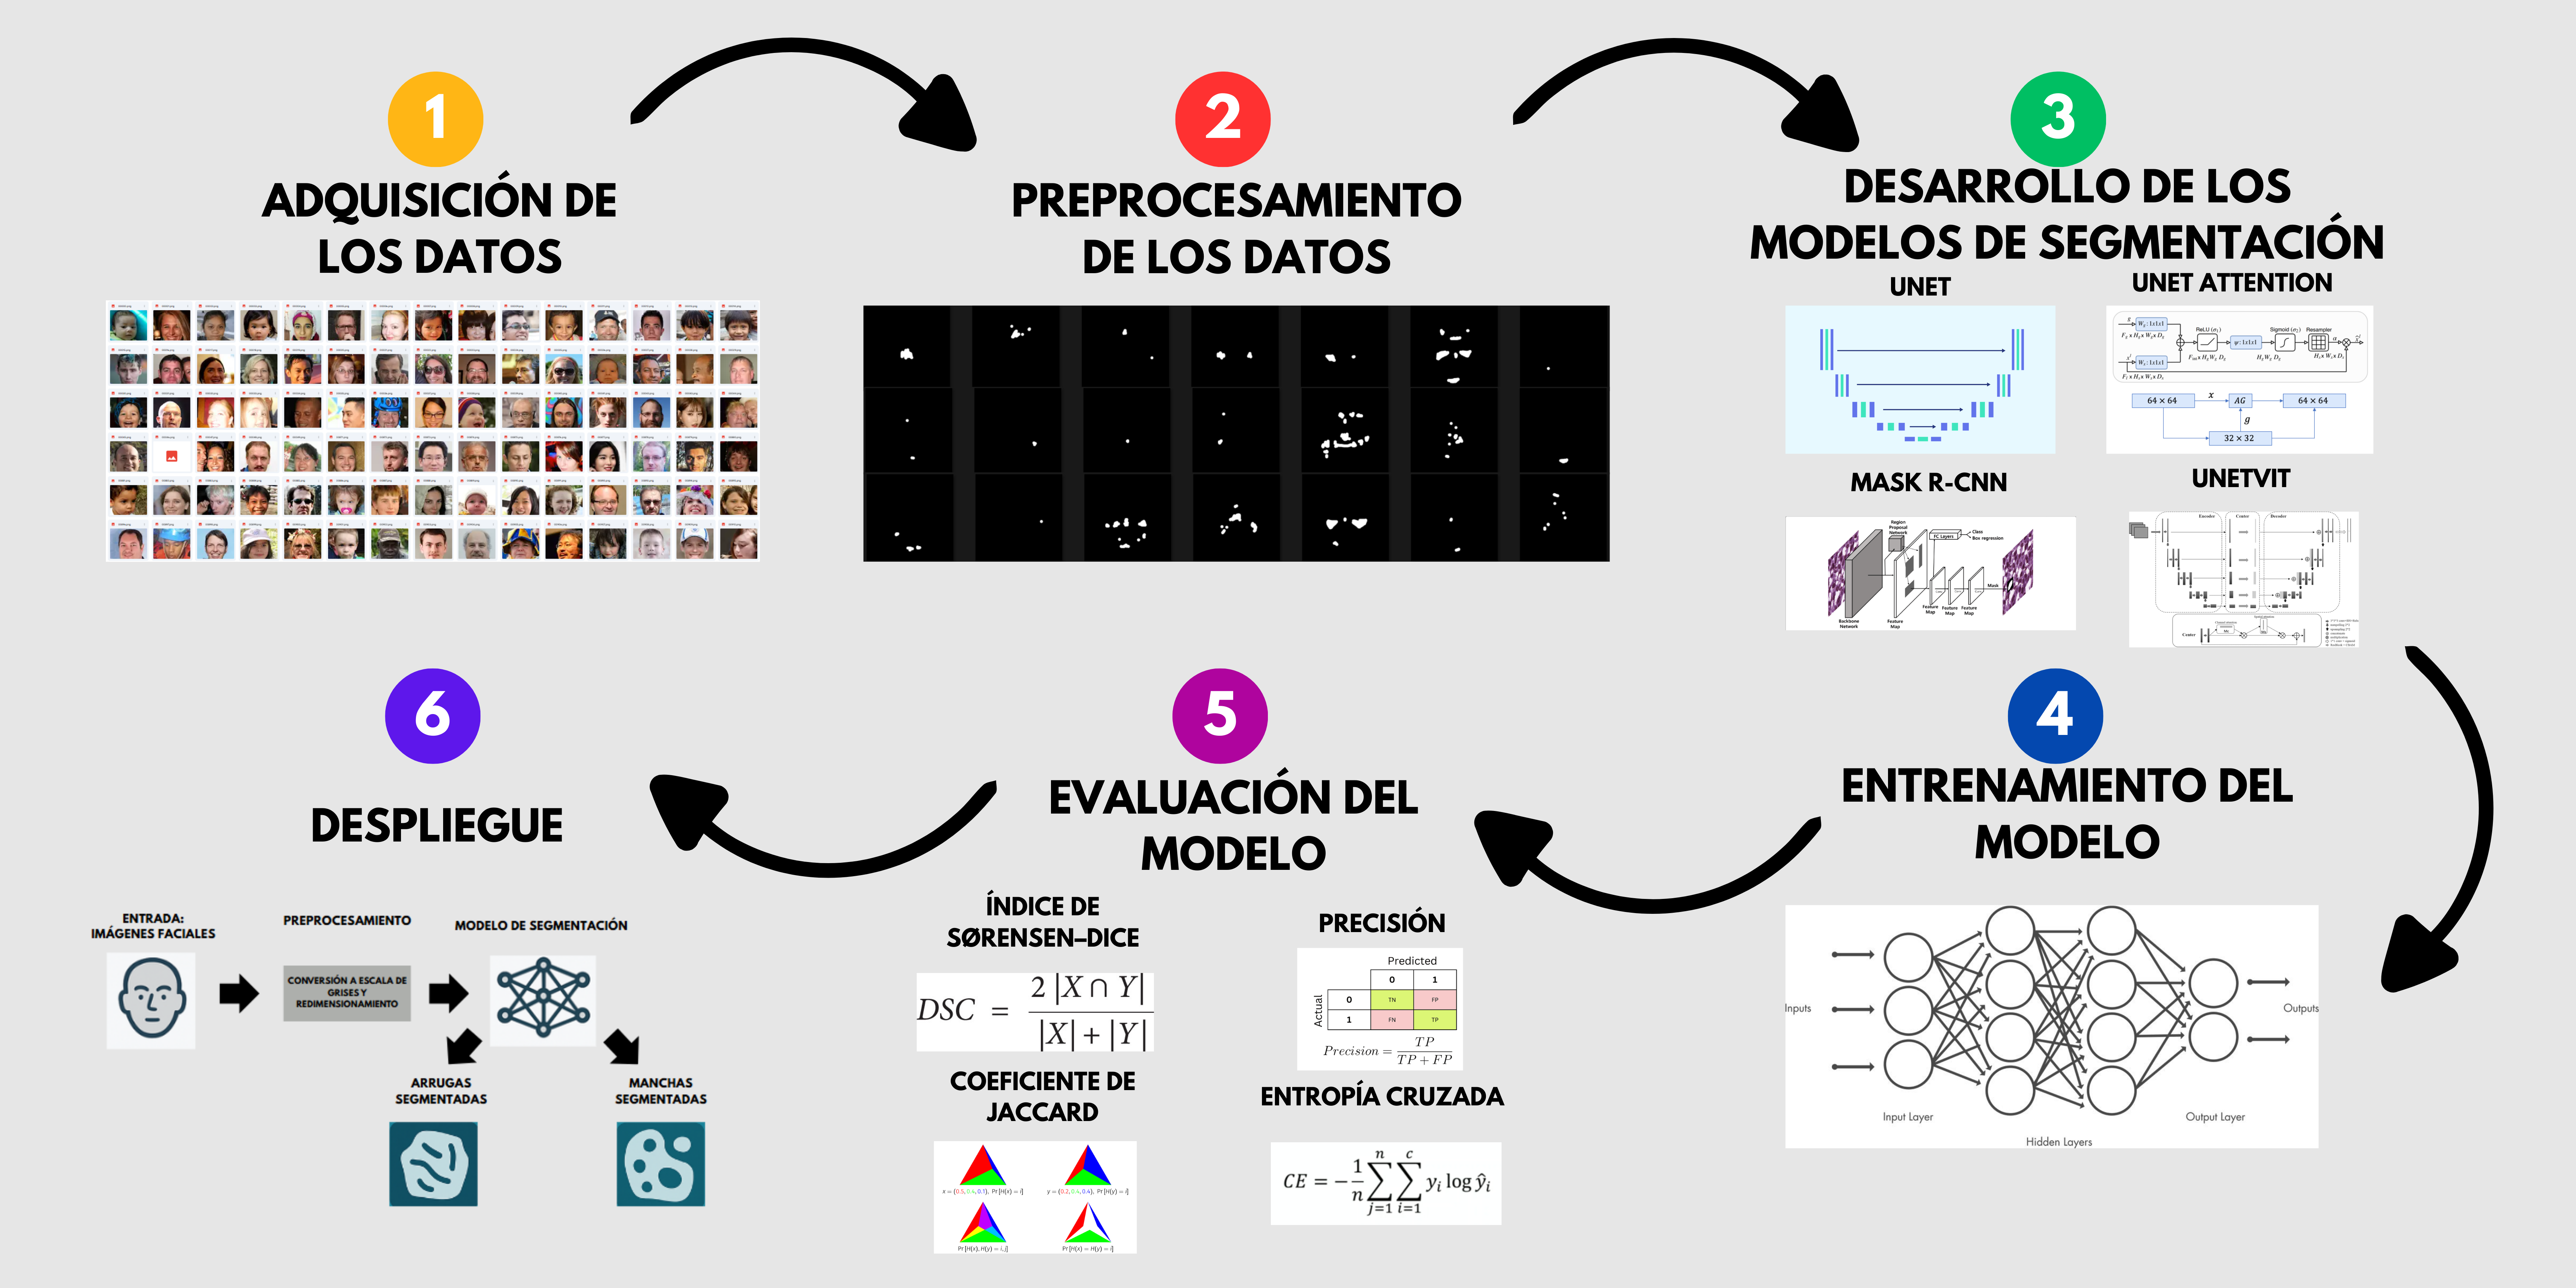
\includegraphics[width=1\textwidth]{3/figures/metodologia.png}
		\caption[Diagrama de Metodología de Investigación]{Diagrama de Metodología de Investigación.\\
			Fuente: Elaboración propia.}
		\label{3:fig3}
	\end{center}
\end{figure}


\subsubsection{Adquisición de los Datos}

En esta sección se describe el procedimiento utilizado para obtener el conjunto de datos empleado en este estudio. A continuación, se presenta una tabla que resume las tareas y actividades realizadas durante esta fase de adquisición. El primer paso fue la recopilación de datos. Los detalles sobre las actividades y tareas se encuentran en la Tabla \ref{tabla:actividades}.

Modelo ensamblado conceptualmente, listo para su implementación en entorno de desarrollo.

\subsubsection{Preprocesamiento de los Datos}
Se realizará el preprocesamiento de las imágenes del conjunto en esta etapa. La tabla \ref{tabla:preprocesamiento} incluye las tareas y actividades necesarias para completar la etapa de preprocesamiento:
\vspace{2ex}


\begin{longtable}{p{3cm}p{3cm}p{9cm}}
    \caption{Actividades de la fase de Preprocesamiento de Datos.}
    \label{tabla:preprocesamiento}\\
    \toprule
    \textbf{Actividades} & \textbf{Descripción} & \textbf{Tareas} \\
    \midrule
    \endfirsthead

    \toprule
    \textbf{Actividades} & \textbf{Descripción} & \textbf{Tareas} \\
    \midrule
    \endhead

    \bottomrule
    \endfoot

    \bottomrule
    \endlastfoot

    Filtración de imágenes faciales con características morfológicas & Eliminación de imágenes con baja resolución, mala iluminación o sin las características morfológicas de interés (arrugas y manchas), para mejorar la calidad del conjunto de datos. & 
    \begin{itemize}
        \item Eliminar imágenes borrosas, sobreexpuestas o subexpuestas.
        \item Conservar solo imágenes con resolución mínima de 128×128 píxeles.
        \item Seleccionar imágenes que contengan al menos una característica morfológica visible: arrugas o manchas.
        \item Verificar que el rostro esté completamente visible y centrado en la imagen.
    \end{itemize} \\

    Representación y normalización de las imágenes faciales & Conversión de las imágenes a formatos adecuados para su análisis por redes neuronales convolucionales. & 
    \begin{itemize}
        \item Redimensionar todas las imágenes a un tamaño uniforme.
        \item Convertir las imágenes a escala de grises o RGB, según el modelo.
        \item Normalizar los valores de píxeles entre 0 y 1.
        \item Aumentar los datos mediante técnicas como rotación, volteo, y zoom para mejorar la generalización.
    \end{itemize} \\

\end{longtable}

\begin{flushleft}
	\small Fuente: Elaboración propia.
\end{flushleft}

Enseguida, se describe en detalle las actividades junto con el resultado esperado.

\textbf{Actividad 1: Filtración de imágenes faciales con características morfológicas}
\\
En la fase de preprocesamiento de datos, la actividad de Filtración se enfoca en depurar y mejorar la calidad del conjunto de datos al eliminar información irrelevante o poco confiable. Esto se logra a través de la eliminación de datos no estándar y la conservación de aquellos que cumplen con criterios específicos de relevancia y fiabilidad. 

\textbf{Entregable}: Conjunto de datos filtrado y optimizado para su posterior análisis.

\textbf{Actividad 2: Representación y normalización de las imágenes faciales}
\\
Por otro lado, la actividad de Representación se encarga de convertir los datos en un formato visual o estructurado más adecuado para su análisis y comprensión. Esto implica transformar los datos en imágenes o representaciones gráficas que faciliten su visualización y entendimiento, contribuyendo así a una mejor interpretación por parte de los usuarios finales, como podemos observar en la Figura \ref{3:fig4}.

\textbf{Entregable}: Representación visual y estructurada de cada rostro facial en un formato adecuado para su procesamiento y análisis posterior.

\begin{figure}[h]
     \begin{center}
         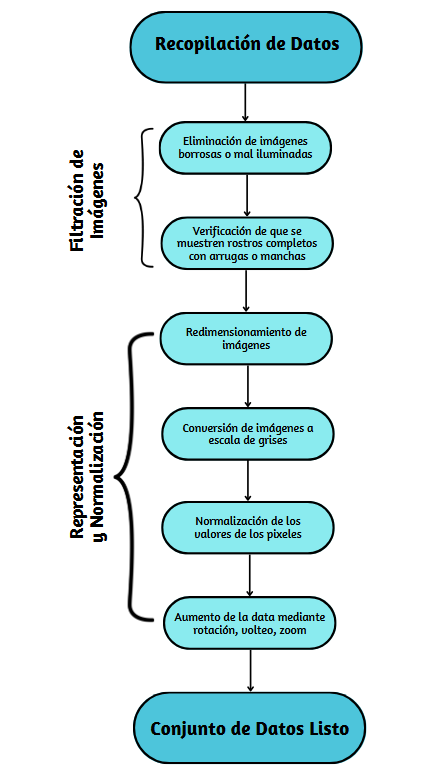
\includegraphics[width=0.75\textwidth]{3/figures/Diagrama de preprocesamiento.png}
         \caption[Diagrama de Preprocesamiento de los Datos]{Diagrama de Preprocesamiento de los Datos.\\
         Fuente: Elaboración propia}
         \label{3:fig4}
     \end{center}
 \end{figure}


 \subsubsection{Desarrollo de los Modelos de Segmentación}
 El desarrollo de los modelos de segmentación de características faciales se estructura en tres actividades clave. Estas actividades incluyen el diseño, implementación y entrenamiento de modelos basados en arquitecturas de redes neuronales profundas como U-Net, ResNet y modelos híbridos con Vision Transformer (ViT). La Tabla \ref{tabla:actividades_segmentacion} presenta el detalle de cada una.

 \vspace{2ex}
 \begingroup
 \renewcommand\arraystretch{1.2}
 \begin{longtable}{p{4cm} p{6cm} p{6cm}}
 \caption{Actividades de la fase de Desarrollo del Modelo de Segmentación.}
 \label{tabla:actividades_segmentacion}\\
 \toprule
 \textbf{Actividades} & \textbf{Descripción} & \textbf{Tareas} \\
 \midrule
 \endfirsthead
 
 \toprule
 \textbf{Actividades} & \textbf{Descripción} & \textbf{Tareas} \\
 \midrule
 \endhead
 
 \bottomrule
 \endfoot
 
 Diseño de la arquitectura del modelo & Selección conceptual y estructural de modelos apropiados para la segmentación de características morfológicas faciales. &
 \begin{itemize}
     \item Análisis de U-Net para segmentación precisa de áreas pequeñas como arrugas y poros.
     \item Evaluación del potencial de ResNet para representar características profundas y complejas.
     \item Consideración de arquitecturas híbridas que integren CNN con Vision Transformer (ViT).
 \end{itemize} \\
 
 Definición de componentes del modelo & Establecimiento de las partes esenciales del modelo para la segmentación de imágenes faciales. &
 \begin{itemize}
     \item Diseño de capas convolucionales, de codificación y decodificación.
     \item Propuesta de bloques residuales y mecanismos de atención en modelos híbridos.
     \item Configuración de dimensiones de entrada y salida adaptadas a imágenes faciales.
 \end{itemize} \\
 
 Estrategia de ensamblado del modelo & Organización lógica y estructural de los bloques que conforman cada arquitectura seleccionada. &
 \begin{itemize}
     \item Integración de módulos especializados según la arquitectura (por ejemplo, skip connections en U-Net).
     \item Planificación de rutas de información para mejorar la segmentación espacial.
     \item Definición de la estructura jerárquica de procesamiento de la imagen.
 \end{itemize} \\
 
 \end{longtable}
 \endgroup

 Enseguida, se proporciona en la Figura \ref{3:fig5} el diagrama de cada actividad, y a su vez un detalle de la actividad junto con el entregable correspondiente que se espera obtener.
 
 \textbf{Actividad 1: Diseño de la arquitectura del modelo}
 \\
 Durante esta etapa se define la estructura general de las redes neuronales que se utilizarán para la segmentación de características morfológicas faciales. El objetivo es seleccionar arquitecturas que sean adecuadas para extraer información precisa de regiones faciales como arrugas, poros o manchas.
 Entre las arquitecturas consideradas se encuentra U-Net, que destaca por su capacidad de segmentación precisa gracias a su estructura simétrica y sus conexiones de salto entre el codificador y el decodificador. También se evalúa el uso de ResNet, una arquitectura que incorpora bloques residuales para mejorar el aprendizaje en redes profundas, especialmente útil para capturar texturas complejas. Asimismo, se contempla la exploración de modelos híbridos que combinan Redes Neuronales Convolucionales (CNN) con Vision Transformer (ViT), lo cual permite captar patrones sutiles mediante mecanismos de atención.
 
 \textbf{Entregable}: Selección de la arquitectura óptima para el modelo de segmentación facial, justificada técnicamente.

 \textbf{Actividad 2: Definición de componentes del modelo}
 \\
Esta actividad consiste en establecer los elementos esenciales que conformarán las redes previamente seleccionadas. Se determina la cantidad de capas, el tipo de operaciones dentro de cada módulo y la forma en que se conectan entre sí, en función de las necesidades de segmentación facial.

En U-Net, por ejemplo, se define cuántas capas de codificación y decodificación se utilizarán, así como las conexiones que transmitirán información detallada entre estas. En ResNet, se especifica el número de bloques residuales y la profundidad de la red, asegurando que se mantenga la eficiencia del aprendizaje sin perder información relevante. En los modelos híbridos con ViT, se determina cómo integrar los módulos de atención con las capas convolucionales, de forma que se mantenga un flujo eficiente de características entre ambos entornos.

 \textbf{Entregable}: Especificación detallada de los componentes y estructura interna de cada arquitectura seleccionada.


 \textbf{Actividad 3: Estrategia de ensamblado del modelo}
 \\
 La última actividad del desarrollo se enfoca en ensamblar los componentes definidos en una arquitectura operativa y coherente. El ensamblado implica organizar los módulos en un orden lógico que permita un flujo fluido de datos desde la entrada hasta la salida del modelo.

Para U-Net, esto implica establecer correctamente las conexiones tipo “skip” que permiten recuperar detalles espaciales perdidos durante la codificación. En el caso de ResNet, se ensamblan los bloques residuales de forma que la información pueda circular libremente entre capas profundas. Finalmente, para los modelos híbridos, se debe asegurar que las características extraídas por las CNN puedan ser procesadas adecuadamente por los módulos de atención del Vision Transformer, logrando así una representación enriquecida para la segmentación facial.

 \textbf{Entregable}: Modelo ensamblado conceptualmente, listo para su implementación en entorno de desarrollo.

 
 \begin{figure}[h]
    \begin{center}
        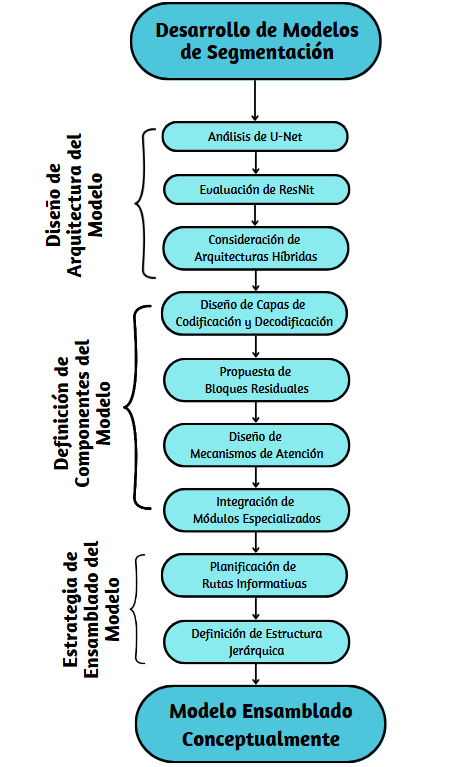
\includegraphics[width=0.75\textwidth]{3/figures/Diagrama de Desarrollo.png}
        \caption[Diagrama del Desarrollo de los Modelos de Segmentación]{Diagrama del Desarrollo de los Modelos de Segmentación.\\
        Fuente: Elaboración propia}
        \label{3:fig5}
    \end{center}
\end{figure}

\subsubsection{Entrenamiento del Modelo}
Al concluir la etapa de Desarrollo de Modelos de Segmentación, se continua con el Entrenamiento, en la Tabla \ref{tabla:entrenamiento_modelo} fue diseñada siguiendo las actividades.

\vspace{2ex}
 \begingroup
 \renewcommand\arraystretch{1.2}
 \begin{longtable}{p{4cm} p{6cm} p{6cm}}
 \caption{Actividades de la fase de Entrenamiento del Modelo.}
 \label{tabla:entrenamiento_modelo}\\
 \toprule
 \textbf{Actividades} & \textbf{Descripción} & \textbf{Tareas} \\
 \midrule
 \endfirsthead
 
 \toprule
 \textbf{Actividades} & \textbf{Descripción} & \textbf{Tareas} \\
 \midrule
 \endhead
 
 \bottomrule
 \endfoot
 
 Configuración del entorno de entrenamiento &
 Preparación del entorno computacional y los recursos necesarios para el entrenamiento del modelo. &
 \begin{itemize}
     \item Selección del framework PyTorch.
     \item Habilitación del uso de GPU para acelerar el entrenamiento.
     \item Establecimiento de rutas de acceso a los datos y modelos.
 \end{itemize} \\
 
 Aplicación de técnicas de optimización &
 Utilización de métodos que permitan una mejora progresiva del modelo a lo largo de las épocas de entrenamiento. &
 \begin{itemize}
     \item Configuración del optimizador Adam para minimizar la función de pérdida.
     \item Ajuste de tasa de aprendizaje, tamaño de batch y número de épocas.
     \item Monitorización de la evolución del loss y métricas de precisión.
 \end{itemize} \\
 
 Validación cruzada del rendimiento &
 Evaluación del desempeño del modelo utilizando múltiples divisiones del conjunto de datos. &
 \begin{itemize}
     \item División del dataset en k pliegues para pruebas y entrenamiento.
     \item Entrenamiento del modelo en diferentes subconjuntos.
     \item Análisis del promedio de métricas obtenidas para garantizar estabilidad.
 \end{itemize} \\
 
 \end{longtable}
 \endgroup

 Enseguida, se proporciona un detalle de la actividad junto con el entregable correspondiente que se espera obtener.
 
 \textbf{Actividad 1: Configuración del entorno de entrenamiento}
 \\
 Durante esta etapa se prepara el entorno computacional necesario para llevar a cabo el entrenamiento del modelo de segmentación facial. Esto implica elegir el framework de desarrollo adecuado, como PyTorch, que permite implementar arquitecturas de redes neuronales de manera eficiente. Además, se habilita el uso de aceleradores de hardware, como GPU, que reducen considerablemente el tiempo de entrenamiento. También se configuran las rutas para el acceso a los datos de entrada y se definen los parámetros básicos que utilizará el entorno de ejecución.

 \textbf{Entregable}: Entorno de entrenamiento configurado y funcional, listo para ejecutar los modelos definidos.

 \textbf{Actividad 2: Aplicación de técnicas de optimización}
 \\
 En esta fase se aplican técnicas diseñadas para mejorar el aprendizaje del modelo durante el entrenamiento. Se implementa el optimizador Adam, ampliamente utilizado por su capacidad de ajustar dinámicamente los parámetros de la red, favoreciendo una convergencia más rápida y estable. Se determinan parámetros críticos como la tasa de aprendizaje, el tamaño del lote (batch size) y el número total de épocas, adaptándolos al comportamiento del modelo y la complejidad del conjunto de datos. Además, se monitorean continuamente la función de pérdida (loss) y las métricas de precisión para evaluar el progreso del modelo.

 \textbf{Entregable}: Modelo entrenado con parámetros de optimización ajustados, y registro de métricas de desempeño durante las épocas.

 \textbf{Actividad 3: Validación cruzada del rendimiento}
 \\
 El objetivo de esta actividad es evaluar de manera robusta el rendimiento del modelo mediante la técnica de validación cruzada. Se divide el conjunto de datos en k pliegues, permitiendo entrenar y validar el modelo en diferentes combinaciones de subconjuntos. Esta estrategia ayuda a prevenir el sobreajuste (overfitting) y asegura que el desempeño del modelo no dependa exclusivamente de una sola partición del dataset. Finalmente, se analiza el promedio de métricas obtenidas en cada iteración para validar la estabilidad y generalización del modelo.

 \textbf{Entregable}: Reporte de resultados de validación cruzada con métricas promedio y análisis de estabilidad del modelo.

\subsubsection{Evaluación del Modelo}
En esta etapa, se lleva a cabo la evaluacion de los prototipos elaborados en este trabajo, en la seccion 3.3.2 se está empleando las métricas de clasificación seleccionadas y detalladas. Se ofrece un analisis pormenorizado de las actividades y tareas ejecutadas en esta fase en la Tabla \ref{tabla:evaluacion_modelo}.

\vspace{2ex}
 \begingroup
 \renewcommand\arraystretch{1.2}
 \begin{longtable}{p{4cm} p{6cm} p{6cm}}
 \caption{Actividades de la fase de Evaluación del Modelo.}
 \label{tabla:evaluacion_modelo}\\
 \toprule
 \textbf{Actividades} & \textbf{Descripción} & \textbf{Tareas} \\
 \midrule
 \endfirsthead
 
 \toprule
 \textbf{Actividades} & \textbf{Descripción} & \textbf{Tareas} \\
 \midrule
 \endhead
 
 \bottomrule
 \endfoot
 
 Preparación de Datos de Validación & Seleccionar y preparar un conjunto de datos de validación representativo. & 
 \begin{itemize}
     \item Elección de imágenes que no hayan sido empleados en el proceso de entrenamiento.
     \item Preprocesamiento de imágenes.
 \end{itemize} \\
 
 Definición de Métricas de Evaluación & Definir métricas cuantitativas para evaluar al modelo de segmentación. & 
 \begin{itemize}
     \item Identificación de métricas adecuadas.
     \item Implementación de funciones para calcular estas métricas.
 \end{itemize} \\
 
 Evaluación del Modelo & Evaluar el modelo entrenado en el conjunto de datos de validación para obtener una línea base. & 
 \begin{itemize}
     \item Eficiencia del modelo de segmentación en el conjunto de validación.
     \item Cálculo de métricas de evaluación.
 \end{itemize} \\
 
 \end{longtable}
 \endgroup

 \textbf{Actividad 1: Preparación de Datos de Validación}
 \\
 La preparación de los datos de validación desempeña un papel crucial en la evaluación de la efectividad del modelo en datos no previamente vistos. Esta tarea implica seleccionar un subconjunto representativo del conjunto de datos que no se haya utilizado durante el entrenamiento del modelo. La selección debe tener en cuenta la diversidad en las imágenes y sus configuraciones para garantizar que el modelo pueda generalizar correctamente a diferentes escenarios.
 
 \textbf{Entregable}: Un conjunto de datos listo para su uso en la evaluación del modelo, que incluye imágenes preprocesadas y listas para ser utilizadas en el análisis.
 
 \textbf{Actividad 2: Definición de Métricas de Evaluación}
 \\
 Para evaluar el rendimiento del modelo de manera cuantitativa, es esencial definir métricas claras. Estas métricas proporcionarán una base objetiva para comparar el rendimiento del modelo en diferentes escenarios y con otros enfoques existentes.
 
 \textbf{Entregable}: Un documento detallado que describe cada métrica y proporciona el código o las funciones necesarias para calcularlas.
 
 \textbf{Actividad 3: Evaluación del Modelo}
 \\
 La evaluación del modelo involucra el uso del conjunto de datos de validación para establecer un punto de referencia sobre su rendimiento. Esta evaluación es esencial para comprender el comportamiento del modelo en situaciones no previamente vistas durante el entrenamiento y para identificar posibles áreas de mejora.
 
 \textbf{Entregable}: Un informe que presenta los resultados de la evaluación inicial, incluyendo las métricas de rendimiento calculadas y cualquier observación relevante sobre el comportamiento del modelo.
 
\subsubsection{Despliegue}
Al concluir la metodología empleada, se procedió a implementar el modelo propuesto luego de finalizar su entrenamiento y evaluación correspondiente. Los pasos y tareas realizados en esta fase se encuentran detallados en la Tabla \ref{tabla:despliegue}.

\vspace{2ex}
 \begingroup
 \renewcommand\arraystretch{1.2}
 \begin{longtable}{p{4cm} p{6cm} p{6cm}}
 \caption{Actividades de la fase de Despliegue.}
 \label{tabla:despliegue}\\
 \toprule
 \textbf{Actividades} & \textbf{Descripción} & \textbf{Tareas} \\
 \midrule
 \endfirsthead
 
 \toprule
 \textbf{Actividades} & \textbf{Descripción} & \textbf{Tareas} \\
 \midrule
 \endhead
 
 \bottomrule
 \endfoot
 
 Preparación del Entorno de Despliegue & Configurar el entorno necesario para desplegar el modelo en producción. & 
    \begin{itemize}
        \item Selección de infraestructura.
        \item Configuración del entorno de hardware y software.
        \item Pruebas iniciales.
    \end{itemize} \\
 
 Despliegue del Modelo en Producción & Implementar el modelo en el entorno de producción para su uso real. & 
 \begin{itemize}
     \item Implementación del modelo en producción.
     \item Configuración de parámetros en tiempo de ejecución.
     \item Monitoreo inicial del desempeño.
 \end{itemize} \\
 \end{longtable}
 \endgroup

\textbf{Actividad 1: Preparación del Entorno de Despliegue}
\\
La preparación del entorno de despliegue es una etapa fundamental para asegurar que el modelo de segmentación pueda ser ejecutado eficientemente en producción. Este proceso implica la selección y configuración de la infraestructura necesaria, incluyendo tanto hardware como software, y la realización de pruebas iniciales para confirmar que todo funciona correctamente antes del despliegue completo.

\textbf{Entregable}: Un entorno completamente preparado, con todos los componentes necesarios instalados y configurados, listo para el despliegue del modelo.

\textbf{Actividad 2: Despliegue del Modelo en Producción}
\\
El despliegue del modelo en producción es el paso en el que el modelo de segmentación se pone en funcionamiento en el entorno de producción. Este proceso incluye la implementación del modelo, la configuración de parámetros necesarios para su ejecución en tiempo real, y el monitoreo inicial para asegurar que el modelo funciona correctamente en condiciones reales.

\textbf{Entregable}: El modelo está completamente implementado y operando en el entorno de producción, con los parámetros ajustados y el desempeño monitoreado para asegurar su correcto funcionamiento.

\section{Metodología para la Medición de Resultados de la Implementación}

Diversas métricas se emplean para evaluar el desempeño de un modelo, en los datos de la Matriz de Confusión, sirviendo como herramientas de evaluación fundamentadas. A continuación, se describe su significado y sus componentes.

\begin{itemize}
\item \textbf{Matriz de confusión}: Tabla de dimensiones que sintetiza la precisión de predicciones generadas por un protitopo de categorización. La matriz muestra la relación entre las etiquetas predichas por el modelo y las etiquetas reales de los datos. Uno de los ejes de la matriz representa las etiquetas predichas, mientras que el otro muestra las etiquetas reales, con N representando el número total de clases. Su propósito primario es analizar la eficacia de un modelo de Aprendizaje Automático Supervisado en conjuntos de datos de prueba, donde las etiquetas reales son desconocidas. El término <<matriz de confusión>> se origina porque ayuda a identificar dónde el sistema confunde entre dos clases (Big Data, 2019). en la Figura \ref{3:fig7}, se puede encontrar una representación visual de la matriz de confusión.
\begin{figure}[H]
	\centering
	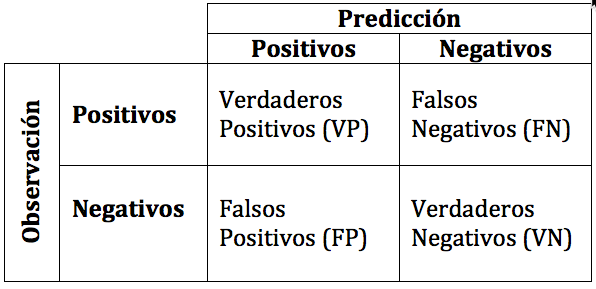
\includegraphics[width=0.75\textwidth]{3/figures/matriz_confusion.png}
	\caption[Matriz de Confusión]{Matriz de Confusión.\\ Fuente: \cite{izco2018bdc}. \citetitle{izco2018bdc}.}
	\label{3:fig7}
\end{figure}
\end{itemize}

\begin{itemize}
    \item \textbf{Verdaderos Positivos}: Se denomina verdadero positivo cuando el modelo realiza una predicción precisa de la clase positiva.
    \item \textbf{Verdaderos Negativos}: Se trata de un verdadero negativo cuando el modelo realiza una predicción correcta de la clase negativa.
    \item \textbf{Falsos Positivos}: Ocurre un falso positivo cuando el modelo hace una predicción incorrecta de la clase positiva. 
    \item \textbf{Falsos Negativos}: Ocurre un falso negativo cuando el modelo hace una predicción incorrecta de la clase negativa. 
    \end{itemize}

Después de explicar los conceptos anteriores, se obtienen diferentes métricas, de las cuales solo se utilizará la precisión métrica según lo referenciado en los documentos anteriores:

\textbf{Precisión}: evalúa la fracción de elementos detectados adecuadamente como positivos entre todos los elementos identificados como positivos. Su cálculo se basa en la siguiente expresión.
        \begin{equation}\label{eq:precision}
            \phantomsection
            \text{Precisión}=\frac{V.P.}{V.P.+F.P.}
            \end{equation}
        \myequations{Fórmula para la precisión}
        
        La pregunta que responde esta métrica es: ¿Cuál es la proporción de segmentaciones positivas que son precisas?


Además, hemos tomado otra métricas para evaluar el rendimiento del modelo de segmentación, las cuales se explicarán a continuación:

\textbf{Índice de Sørensen–Dice (Dice Similarity Coefficient - DSC)}
El índice de Sørensen-Dice es una medida estadística utilizada para evaluar la similitud entre dos muestras. En el contexto de segmentación de imágenes, cuantifica la superposición entre la segmentación predicha y la verdadera (ground truth). \parencite{taha2015metrics}
        
Se define como:
        
\begin{equation}
    \text{DSC} = \frac{2 \times |A \cap B|}{|A| + |B|}
\end{equation}
\myequations{Fórmula del Índice de Sørensen–Dice (DSC)}

\noindent Donde:
\begin{itemize}
    \item $|A|$ representa el número de píxeles predichos como positivos por el modelo.
    \item $|B|$ representa el número de píxeles verdaderamente positivos (segmentación real).
    \item $|A \cap B|$ es el número de píxeles correctamente clasificados como positivos (verdaderos positivos).
\end{itemize}

\noindent El Índice de Sørensen–Dice mide la superposición entre la predicción y la verdad real, con un rango de valores entre $0$ (sin coincidencia) y $1$ (coincidencia perfecta).
     

\textbf{Coeficiente de Jaccard (Índice de Intersección sobre Unión - IoU)}
El Coeficiente de Jaccard o IoU (Intersection over Union) mide la proporción de la intersección entre el área segmentada correctamente y la unión de todas las áreas predichas y reales. Es una de las métricas más comunes en segmentación de imágenes. \parencite{reinke2021common}
        
\begin{equation}
    \text{IoU} = \frac{|A \cap B|}{|A \cup B|}
\end{equation}
\myequations{Fórmula del Coeficiente de Jaccard (Intersection over Union)}

\noindent Donde:
\begin{itemize}
    \item $|A|$ es el conjunto de píxeles positivos predichos.
    \item $|B|$ es el conjunto de píxeles positivos reales.
    \item $|A \cap B|$ representa los píxeles clasificados correctamente como positivos (verdaderos positivos).
    \item $|A \cup B|$ representa el total de píxeles positivos predichos o reales (la unión de ambos conjuntos).
\end{itemize}

\noindent El Coeficiente de Jaccard mide la proporción de superposición respecto al total combinado de las regiones predicha y real.
                     
El Coeficiente de Jaccard tiende a ser más estricto que el índice de Dice, ya que penaliza con mayor fuerza las falsas predicciones. Se considera una métrica robusta para segmentaciones de alta precisión. \parencite{reinke2021common}

\textbf{Entropía Cruzada (Cross-Entropy Loss)}
La entropía cruzada es una función de pérdida ampliamente usada para tareas de clasificación y segmentación semántica, especialmente cuando se aplica un modelo que produce probabilidades para cada clase (como softmax o sigmoid). \parencite{goodfellow2016deep}

\begin{equation}
    \text{CE} = -\sum_{i=1}^{N} y_i \log(\hat{y}_i)
\end{equation}
\myequations{Fórmula de Entropía Cruzada (Cross-Entropy Loss)}

\noindent Donde:
\begin{itemize}
    \item $N$ es el número total de muestras (píxeles o instancias).
    \item $y_i$ es la etiqueta verdadera de la clase para la muestra $i$.
    \item $\hat{y}_i$ es la probabilidad predicha por el modelo para esa clase.
\end{itemize}

\noindent La Entropía Cruzada penaliza más fuertemente las predicciones con alta confianza que resultan incorrectas, y se minimiza durante el entrenamiento del modelo.

En segmentación binaria, esta función penaliza más las clasificaciones incorrectas cuanto más seguras son las predicciones erróneas. Se considera una métrica adecuada para entrenar redes neuronales cuando se requiere distinguir entre fondo y objeto. \parencite{goodfellow2016deep}

\begin{landscape}
	\section{Cronograma de actividades y presupuesto}
	Se propuso un cronograma para la investigación. Conforma desde el inicio hasta ser terminada con la sustentación final planeada para mediados del año 2024. Este se presneta en la Figura \ref{3:fig6}.

	\begin{figure}[!ht]
		\begin{center}
			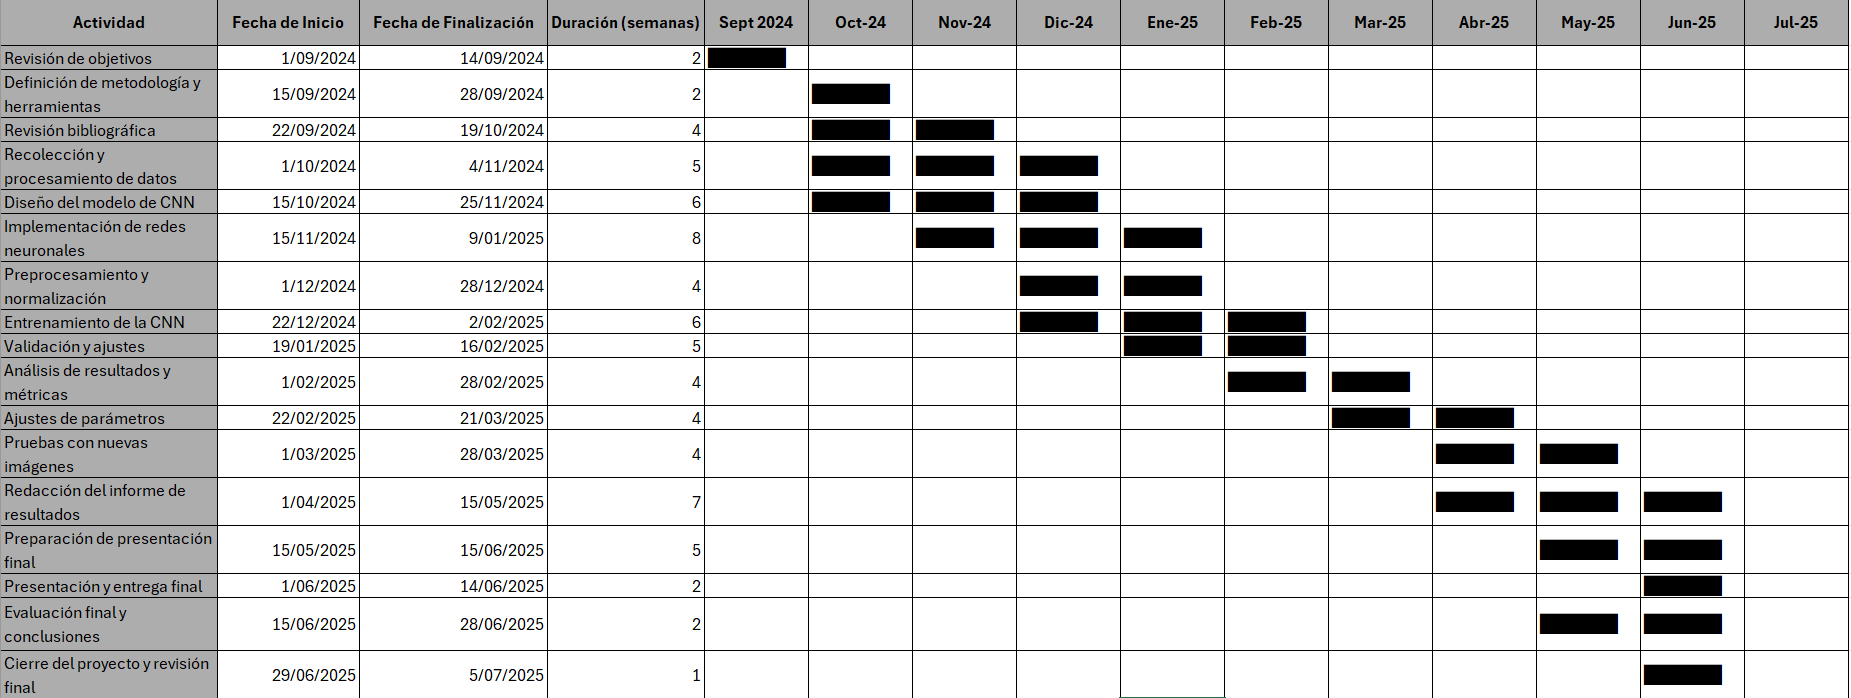
\includegraphics[width=1.50\textwidth]{3/figures/gant.png}
			\caption[Cronograma de actividades]{Cronograma de actividades.\\
				Fuente: Elaboración propia.}
			\label{3:fig6}
		\end{center}
	\end{figure}
	
\end{landscape}
%%%%%%%%%%%%%%%%%%%%%%%%%%%%%%%%%%%%%%%%

%%%%%%%%%%%%%%%%%%%%%%%%%%%%%%%



La Tabla \ref{tab:presupuesto} detalla los gastos relacionados con la investigación, incluyendo la compra de herramientas como una computadora portátil antes del inicio del proyecto, así como los costos asociados a actividades generales y al proceso de redacción y presentación pública de la tesis.

\begin{table}[h!]
	\caption{Presupuesto}
	\label{tab:presupuesto}
	\centering
	\small
	\begin{tabular}{p{6cm}rrr}
		\toprule
		\textbf{Concepto} & \textbf{Horas empleadas} & \textbf{Gasto (en soles)} & \textbf{Total} \\
		\midrule
		\multicolumn{4}{l}{\textbf{Activos físicos}} \\
		Portátil Lenovo Ideapad S340-15IIL Core i7 de 10ma GEN & -- & S/.5,700.00 & S/.5,700.00 \\
		\midrule
		\multicolumn{4}{l}{\textbf{Honorarios por el proceso de elaboración y defensa pública de la tesis}} \\
		Tasa de registro para el tema de investigación & -- & S/.800.00 & S/.800.00 \\
		Apartado del tema de tesis & -- & S/.2,700.00 & S/.2,700.00 \\
		Honorarios de defensa & -- & S/.1,500.00 & S/.1,500.00 \\
		\midrule
		\multicolumn{4}{l}{\textbf{Personal o equipo humano}} \\
		Progreso de tesis & 1000 & Inconmensurable & -- \\
		\midrule
		\multicolumn{4}{l}{\textbf{Gastos operativos}} \\
		Conexión a internet y servicio de electricidad (durante 8 meses) & 200 & S/.50.00 & S/.1000.00 \\
		\midrule
		\textbf{Python} & 50 & - & - \\
		\midrule
		\textbf{Suma total} & 1250 & -- & S/.11,700.00 \\
		\bottomrule
	\end{tabular}
	\begin{flushleft}
		\small Fuente: Elaboración propia.
	\end{flushleft}
\end{table}





%\chapter{Desarrollo de la Solución}
Dentro de esta sección se expone con precisión el procedimiento descrito previamente en la sección anterior, correspondiente a cada acción incluida en la metodología implementada, junto con los entregables previstos.

\section{Adquisición de los Datos}

\textbf{Actividad 1: Identificación de la data que contengan imágenes de rostros con características morfológicas faciales de proporciones similares}
 
Con el objetivo de entrenar un modelo de segmentación enfocado en características morfológicas faciales como arrugas y manchas, se llevó a cabo una exhaustiva búsqueda de bases de datos públicas en repositorios especializados. Se priorizó la recolección de conjuntos de datos que incluyeran imágenes faciales en alta resolución, variedad de edades, géneros y tonos de piel, así como condiciones de iluminación lo suficientemente controladas como para facilitar la segmentación de detalles faciales sutiles.

Durante este proceso, se identificaron diversos repositorios en plataformas como GitHub que ofrecían acceso a bases de datos con más de 200,000 imágenes faciales. Entre los conjuntos más destacados se encuentran versiones extendidas de datasets como CelebA, FFHQ (Flickr-Faces-HQ), y otros compendios curados por la comunidad investigadora, que contienen imágenes faciales etiquetadas o anotadas para tareas de reconocimiento y análisis facial.

Sin embargo, debido al enfoque específico de esta investigación la segmentación de características morfológicas finas como arrugas y manchas fue necesario realizar una selección cuidadosa de las imágenes más adecuadas. Para ello, se aplicaron criterios de claridad visual, resolución suficiente y visibilidad explícita de las deformaciones morfológicas faciales. Como resultado de este filtrado, se seleccionó un subconjunto compuesto por 5,000 imágenes faciales que cumplían con los siguientes criterios:

\begin{itemize}
    \item Alta calidad visual.   
    \item Visibilidad clara de texturas de la piel.
    \item Presencia evidente de arrugas y manchas.
    \item Proporciones faciales dentro de un rango estándar para facilitar el modelado.
\end{itemize} 

Este conjunto reducido pero representativo,lo podemos ver en la Figura \ref{4:fig1}, constituye la base de entrenamiento y validación del modelo propuesto. La selección manual de estos datos buscó optimizar el desempeño del modelo, al exponerlo exclusivamente a ejemplos que contienen información útil para aprender patrones asociados a las características morfológicas de interés.

\begin{figure}[h]
	\begin{center}
		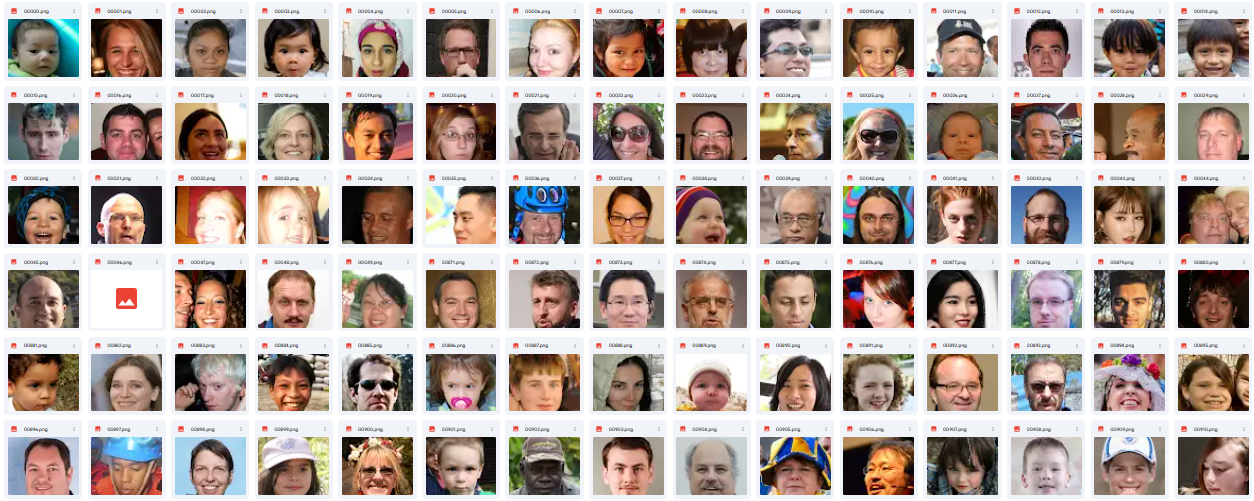
\includegraphics[width=0.75\textwidth]{4/figures/data.png}
		\caption[Dataset recolectado de repositorios]{Dataset recolectado de repositorios.\\
		Fuente: Elaboración propia}
		\label{4:fig1}
	\end{center}
\end{figure}

\section{Preprocesamiento de los Datos}

\textbf{Actividad 1: Filtración de imágenes faciales con características morfológicas}

Una vez recopilado el subconjunto de 5,000 imágenes faciales con características morfológicas visibles, se procedió a una etapa de filtración adicional orientada a reforzar la consistencia y la relevancia de los datos para la tarea de segmentación. Esta filtración se enfocó en garantizar que todas las imágenes seleccionadas contuvieran arrugas y manchas claramente identificables, descartando aquellas que, pese a su calidad visual, no presentaban estas características de manera explícita.

El proceso se realizó mediante una inspección semiautomática, apoyada en técnicas básicas de detección de texturas y realce de bordes para facilitar la identificación visual de las zonas con deformaciones. Como resultado, se aseguraron condiciones homogéneas entre las imágenes del dataset final, lo que permitió una base sólida para la generación de máscaras de segmentación precisas.

\textbf{Actividad 2: Representación y normalización de las imágenes faciales}

Con el conjunto de imágenes definitivo, se ejecutó un proceso de preprocesamiento estandarizado con dos objetivos principales: uniformar las dimensiones espaciales de las imágenes y generar las máscaras binarias asociadas a las regiones con deformaciones morfológicas.

En primer lugar, todas las imágenes fueron redimensionadas a una resolución uniforme de 1024x1024 píxeles, preservando la relación de aspecto y aplicando interpolación bilineal para mantener la calidad visual. Esta estandarización es fundamental para asegurar la compatibilidad estructural con las redes neuronales convolucionales utilizadas en etapas posteriores, y facilita la aplicación de operaciones convolucionales sobre áreas homogéneas.

En segundo lugar, se generaron máscaras binarias (en blanco y negro) correspondientes a cada imagen. Estas máscaras representan las regiones específicas del rostro que contienen arrugas, manchas u otras alteraciones morfológicas, codificadas de la siguiente manera:

\begin{itemize}
    \item Blanco (valor 1): Regiones con características morfológicas relevantes (objetivo de segmentación).   
    \item Negro (valor 0): Regiones sin interés morfológico.
\end{itemize} 

Las máscaras, como se ve en la Figura \ref{4:fig2}, fueron elaboradas a partir de una combinación de anotación semiautomática y herramientas de realce de texturas, contrastes y gradientes, con verificación manual en una muestra aleatoria para asegurar su validez.

\begin{figure}[h]
	\begin{center}
		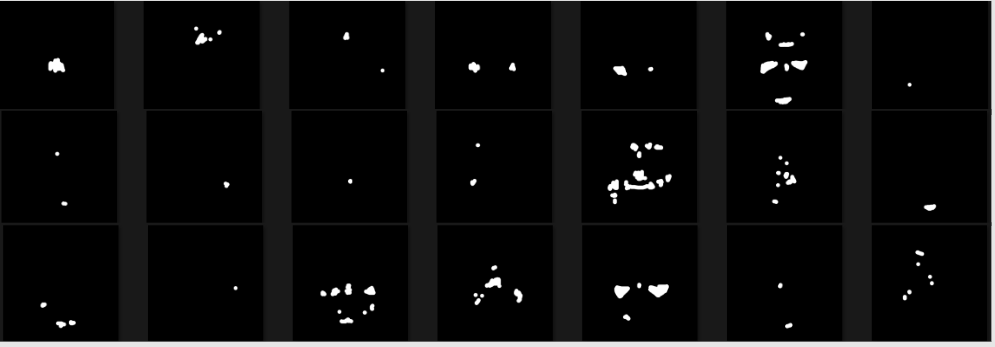
\includegraphics[width=0.75\textwidth]{4/figures/mascaras.png}
		\caption[Máscaras binarias generadas]{Máscaras binarias generadas.\\
		Fuente: Elaboración propia}
		\label{4:fig2}
	\end{center}
\end{figure}

Este proceso de representación y normalización, como se ve en el diagrama final de Preprocesamiento en la Figura \ref{4:fig3}, permitió convertir los datos originales en pares de entrada (imagen facial) y salida (máscara de segmentación), aptos para el entrenamiento supervisado del modelo de segmentación basado en redes neuronales convolucionales.

\begin{figure}[h]
	\begin{center}
		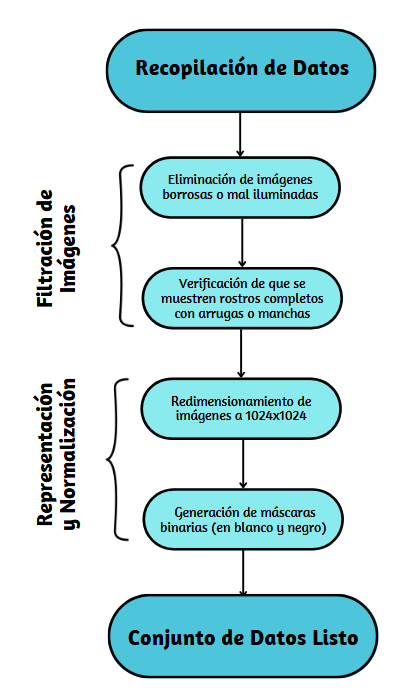
\includegraphics[width=0.45\textwidth]{4/figures/diagrama final prepo.png}
		\caption[Diagrama de Preprocesamiento Utilizado]{Diagrama de Preprocesamiento Utilizado.\\
		Fuente: Elaboración propia}
		\label{4:fig2}
	\end{center}
\end{figure}

\section{Desarrollo de los Modelos de Segmentación}

\textbf{Actividad 1: Diseño de la arquitectura del modelo}\\
Se diseñó una arquitectura basada en U-Net con Attention Gates, que consta de:
\begin{itemize}
  \item Módulos de doble convolución (DoubleConv) en el encoder y decoder.  
  \item Capas de atención (AttentionGate) ubicadas en cada salto del decoder para realzar las regiones de interés (arrugas y manchas).  
  \item Caminos de downsampling (MaxPool2d) y upsampling (ConvTranspose2d) para conservar la resolución espacial.  
  \item Capa final de convolución 1x1 para segmentación en tres clases (fondo, arrugas, manchas).  
\end{itemize}

\textbf{Actividad 2: Definición de componentes del modelo}\\
Los componentes principales incluyen:
\begin{itemize}
  \item \textit{DoubleConv}: bloque de dos convoluciones secuenciales con BatchNorm y ReLU.  
  \item \textit{AttentionGate}: mecanismo de atención consistente en convoluciones 1x1, sumas tensoriales y función Sigmoid para generar máscaras atencionales.  
  \item Optimizador \texttt{AdamW} con decaimiento de pesos para mejorar la generalización.  
  \item Scheduler \texttt{ReduceLROnPlateau} para ajuste dinámico de la tasa de aprendizaje.  
  \item Función de pérdida \texttt{CrossEntropyLoss} con pesos calculados por median frequency balancing.  
\end{itemize}

\textbf{Actividad 3: Estrategia de ensamblado del modelo}\\
Se definió una estrategia de ensamblado simple basada en el entrenamiento de un solo modelo entrenado por 50 épocas, guardando el estado de mejor rendimiento en validación (menor pérdida). No se implementó ensamblado múltiple, pues la arquitectura con atención demostró ser suficiente tras el análisis de métricas.

\section{Entrenamiento del Modelo}

\textbf{Actividad 1: Configuración del entorno de entrenamiento}\\
Se configuró el entorno con los siguientes parámetros:
\begin{itemize}
  \item Ruta de datos: \texttt{face\_images}, \texttt{arrugas}, \texttt{manchas}.  
  \item Tamaño de lote (batch size): 4.  
  \item Dimensión de entrada: 256 x 256 píxeles.  
  \item Tasa de aprendizaje inicial: $1\times10^{-4}$.  
  \item Número de épocas: 50.  
  \item Dispositivo de cómputo: GPU (CUDA) o CPU según disponibilidad.  
  \item Semilla aleatoria fija (42) para reproducibilidad.  
\end{itemize}

\textbf{Actividad 2: Aplicación de técnicas de optimización}\\
Se incorporaron las siguientes técnicas:
\begin{itemize}
  \item Aumentos de datos con \texttt{albumentations}: volteos, rotaciones, ruido Gaussiano, brillo/contraste, transformaciones elásticas y desenfoque.  
  \item Balanceo de clases mediante median frequency balancing para generar pesos en \texttt{CrossEntropyLoss}.  
  \item Optimizador \texttt{AdamW} y scheduler \texttt{ReduceLROnPlateau} para ajuste automático de la tasa de aprendizaje.  
  \item Impresión de métricas de pérdida en entrenamiento y validación por época.  
\end{itemize}

\textbf{Actividad 3: Validación cruzada del rendimiento}\\
La validación se realizó con:
\begin{itemize}
  \item División de datos: 80\% entrenamiento, 20\% validación usando \texttt{train\_test\_split}.  
  \item DataLoaders separados para entrenamiento y validación, garantizando evaluación independiente.  
  \item Cálculo de métricas (pérdida, precisión, Dice, Jaccard) en el conjunto de validación cada época.  
  \item Guardado del modelo con menor \emph{val\_loss} como mejor checkpoint.  
\end{itemize}


\section{Evaluación del Modelo}

\textbf{Actividad 1: Preparación de Datos de Validación}\\
Se prepararon las imágenes de validación con transformaciones mínimas:
\begin{itemize}
  \item Redimensionamiento a 256x256 píxeles.  
  \item Conversión a tensor SIN alteraciones adicionales.  
  \item Unión de máscaras de arrugas y manchas en una única máscara multicategoría.  
\end{itemize}

\textbf{Actividad 2: Definición de Métricas de Evaluación}\\
Las métricas utilizadas fueron:
\begin{itemize}
  \item \textit{Precision} (macro) para evaluar la exactitud de las predicciones.  
  \item \textit{Dice Score} promedio para medir la superposición.  
  \item \textit{Jaccard Index (IoU)} promedio para una evaluación estricta del solapamiento.  
\end{itemize}

\textbf{Actividad 3: Evaluación del Modelo}\\
El modelo alcanzó los siguientes resultados en validación:
\begin{itemize}
  \item \textbf{Pérdida mínima (val\_loss):} 0.0458 (época 50).  
  \item \textbf{Precision promedio:} 0.645.  
  \item \textbf{Dice Score promedio:} 0.440.  
  \item \textbf{Jaccard Index promedio:} 0.289.  
  \item Se observaron mejores resultados en la detección de arrugas debido a mayor representación de esta clase.  
  \item La clase ":manchas" mostró métricas ligeramente inferiores, sugiriendo futuras mejoras en aumentos específicos.  
\end{itemize}

Los resultados numéricos y ejemplos de segmentaciones se presentan en la sección de análisis de resultados con gráficas de evolución y comparaciones visuales.


\section{Despliegue}

\textbf{Actividad 1: Preparación del Entorno de Despliegue}

\textbf{Actividad 2: Despliegue del Modelo en Producción}

%\chapter{Conclusiones y Recomendaciones}
\section{Conclusiones}
Una vez definido el problema central relacionado con la segmentación automatizada de deformaciones morfológicas faciales y establecido el marco de objetivos e hipótesis, se logró cumplir con el propósito general de esta investigación: diseñar un sistema capaz de segmentar arrugas y manchas en imágenes faciales mediante Redes Neuronales Convolucionales. Este objetivo se abordó considerando como criterio principal el uso exclusivo de imágenes faciales humanas y, como enfoque metodológico, la implementación de un modelo de aprendizaje profundo basado en redes neuronales convolucionales, específicamente una arquitectura U-Net con mecanismos de atención.

En relación con los objetivos específicos, se evidenció que el análisis de modelos propuestos en investigaciones previas tuvo un impacto significativo en la selección de características relevantes y en la construcción del enfoque metodológico adoptado. Esta revisión permitió validar hipótesis provenientes de la literatura sobre el desempeño superior de arquitecturas basadas en redes neuronales convolucionales frente a enfoques tradicionales de aprendizaje automático, especialmente en tareas de segmentación de imágenes. Los resultados obtenidos, como se ven el Tabla \ref{tab:result_models}, durante las fases de evaluación cuantitativa respaldan esta elección, demostrando mejoras sustanciales en métricas como loss, precisión, Dice Score e IoU.

A partir de los resultados mostrados en la Tabla \ref{tab:result_models}, se concluye que el modelo U-Net con mecanismos de atención obtuvo el mejor desempeño global en la tarea de segmentación de características morfológicas faciales, superando significativamente a sus variantes y a otras arquitecturas evaluadas. Este modelo logró una pérdida (entropía cruzada) de 0.1158 y una precisión de 0.911, posicionándose por encima del U-Net estándar y de U-Net con codificador MiT-B0, así como muy por delante de Mask R-CNN, que mostró un rendimiento considerablemente inferior. Las métricas del índice de Sørensen–Dice (0.810) y el coeficiente de Jaccard (0.852) reflejan la eficacia del modelo propuesto en términos de solapamiento con las segmentaciones reales. Sin embargo, también se identificó que el rendimiento de algunos modelos estuvo condicionado por las características específicas de su diseño. Por ejemplo, el modelo con codificador MiT-B0, pese a incorporar componentes basados en transformadores, presentó dificultades para generalizar, lo que se evidenció en una baja precisión (0.443) y un Dice Score de apenas 0.320. Este comportamiento sugiere que, si bien la arquitectura es prometedora, su desempeño podría estar limitado por el tamaño del conjunto de datos o la sensibilidad a variaciones de iluminación y contraste presentes en las imágenes faciales. Estas observaciones subrayan la importancia de una adecuada selección arquitectónica y del ajuste fino de hiperparámetros en función de las características del problema. En este caso, la integración de mecanismos de atención demostró ser clave para mejorar el enfoque espacial del modelo, potenciando su capacidad para segmentar con mayor precisión regiones como arrugas y manchas en entornos clínicos o cosméticos.

A nivel individual, la aplicación web desarrollada para la segmentación de características morfológicas faciales demostró un comportamiento consistente en todas las métricas de evaluación aplicadas, desde las más convencionales como la precisión global, hasta aquellas más sensibles al desbalance de clases, como el índice de Sørensen–Dice y el coeficiente de Jaccard. El modelo U-Net con atención, integrado en el sistema, fue entrenado sin mayores dificultades y mostró una alta estabilidad durante el proceso, reflejando una baja pérdida de entrenamiento y validación. La arquitectura implementada mantuvo una adecuada capacidad de generalización a pesar de ciertas limitaciones inherentes al conjunto de datos, como variabilidad en la iluminación o diversidad en los tonos de piel. En este sentido, el entorno de inferencia fue capaz de gestionar adecuadamente estos desafíos y generar segmentaciones robustas en la mayoría de los casos evaluados. Esta fiabilidad es especialmente relevante considerando que la aplicación web fue diseñada para operar en tiempo real y con imágenes proporcionadas directamente por el usuario, lo que introduce una mayor heterogeneidad en las entradas. Por último, sí se evidenció que la calidad y resolución de las imágenes puede impactar en la nitidez de las regiones segmentadas, especialmente en manchas de baja intensidad o arrugas poco marcadas. No obstante, el sistema mantuvo métricas altas y estables en todos los ensayos realizados, consolidándose como una herramienta eficaz y funcional tanto para aplicaciones clínicas como cosméticas.

\section{Recomendaciones}

Para mejorar la capacidad de generalización del modelo, se recomienda incrementar el volumen del conjunto de datos, incorporando imágenes faciales con mayor variabilidad en condiciones de iluminación, tono y tipo de piel, presencia de maquillaje y expresiones faciales diversas. La inclusión de muestras procedentes de bases de datos clínicas también podría enriquecer la robustez del sistema frente a casos dermatológicos reales.

Aunque la aplicación fue desarrollada para su uso en entorno web local, se sugiere su adaptación para su ejecución en dispositivos móviles o entornos con recursos computacionales restringidos. Para ello, se podrían explorar técnicas de cuantización o poda de redes, así como la conversión del modelo a formatos ligeros como ONNX o TensorFlow Lite.

Con el fin de mejorar la experiencia del usuario y validar los resultados obtenidos, se propone incorporar un módulo de evaluación automática que permita comparar las máscaras generadas por el modelo con etiquetas reales, en caso de disponer de ellas, o bien aplicar mecanismos de retroalimentación por parte del usuario para ajustar la sensibilidad del modelo.

Si bien la U-Net con atención demostró un excelente rendimiento, futuras investigaciones podrían considerar arquitecturas más recientes como U-Net++, DeepLabV3+, o segmentadores basados en transformadores (p. ej., SegFormer), los cuales han mostrado resultados prometedores en tareas de segmentación médica y facial.

Se recomienda realizar experimentos adicionales de ajuste fino de hiperparámetros como el tamaño del batch, la tasa de aprendizaje y los pesos de clase en la función de pérdida, así como aplicar técnicas como dropout o data augmentation adaptativa, con el fin de minimizar el riesgo de sobreajuste en datasets más extensos.


%\include{6/conclusion}

%%Para insertar los capítulos de forma seguida
\chapter{Planteamiento del Problema}
\section{Descripción de la Realidad Problemática}

La industria cosmética y de cuidado de la piel ha visto un crecimiento exponencial en las últimas décadas. Según datos de Statista, el mercado global de productos para el cuidado de la piel superó los 130 mil millones de dólares en 2023, con una tasa de crecimiento anual compuesta de aproximadamente el 0,045 \parencite{statista2023}. Este auge refleja la creciente demanda por soluciones que permitan a los consumidores mejorar su apariencia, retardar los signos del envejecimiento y solucionar problemas estéticos como las arrugas, los poros dilatados y las manchas faciales.

A pesar de la variedad de productos y tratamientos disponibles en el mercado, persisten varios desafíos relacionados con la evaluación precisa y personalizada de los problemas de la piel. Uno de los mayores obstáculos en la actualidad es la falta de herramientas tecnológicas que permitan realizar un análisis profundo y cuantitativo de las características morfológicas de la piel. Problemas como las arrugas, los poros dilatados y las manchas son difíciles de evaluar de manera objetiva, ya que la mayoría de los diagnósticos aún dependen de la observación manual o de sistemas de análisis que no logran captar las sutilezas y complejidades de la piel facial \parencite{phillips2020}.

La precisión en la detección de estas características es crucial para el desarrollo de tratamientos más efectivos. Por ejemplo, la identificación temprana de las arrugas incipientes permitiría la aplicación de productos antiarrugas de manera preventiva, antes de que las líneas se profundicen. Sin embargo, las evaluaciones actuales a menudo son subjetivas y pueden variar según el profesional o las herramientas utilizadas. En este sentido, estudios recientes han demostrado que las redes neuronales convolucionales (CNN) tienen el potencial de revolucionar la manera en que se realiza la segmentación y análisis de imágenes de piel \parencite{esteva2017}. Estas redes permiten procesar grandes volúmenes de datos visuales y detectar patrones morfológicos con un nivel de precisión que supera las técnicas tradicionales.

Otro desafío significativo es la evaluación de poros y manchas. Los poros dilatados son una preocupación estética común, especialmente entre personas con piel grasa. La falta de herramientas capaces de cuantificar y analizar adecuadamente el tamaño y la densidad de los poros limita las recomendaciones de tratamiento personalizadas \parencite{jia2019}. De manera similar, las manchas faciales, que pueden aparecer debido a la edad, la exposición solar o factores hormonales, requieren una evaluación temprana para evitar su progresión. Las CNN, al especializarse en la segmentación de imágenes, pueden proporcionar una solución eficaz para mapear la distribución y evolución de estas imperfecciones cutáneas \parencite{esteva2017}.

Estadísticamente, se ha encontrado que más del 0,7 de las personas mayores de 25 años muestran algún signo de envejecimiento facial, como arrugas y manchas, lo que impulsa la demanda de productos antiarrugas y despigmentantes \parencite{aad2022}. Sin embargo, el éxito de estos productos depende en gran medida de una evaluación precisa del estado de la piel. Actualmente, los diagnósticos imprecisos o subjetivos pueden llevar a la aplicación de productos inapropiados, lo que no solo afecta la satisfacción del consumidor, sino que también reduce la efectividad de los tratamientos \parencite{khatri2018}.

Este contexto evidencia la necesidad urgente de desarrollar tecnologías avanzadas que mejoren la precisión en la evaluación estética de la piel. Las redes neuronales convolucionales ofrecen una herramienta prometedora para abordar este problema, al permitir una segmentación detallada de las características morfológicas clave de la piel, como arrugas, poros y manchas. El uso de estas tecnologías no solo permitiría mejorar los diagnósticos estéticos, sino que también contribuiría a la creación de tratamientos personalizados más efectivos, incrementando la satisfacción del usuario final.



\section{Formulación del Problema}

\subsection{Problema General}
PG: \newcommand{\ProblemaGeneral}{
¿Cómo afecta la falta de un sistema de segmentación  de características morfológicas de la piel facial en la detección de arrugas, poros y manchas?
}
\ProblemaGeneral
\subsection{Problemas Específicos}
\newcommand{\Pbone}{
¿Cómo se medirá la eficiencia del sistema de segmentación morfológica en la detección de arrugas, poros y manchas?
}
\newcommand{\Pbtwo}{
¿Cómo se desarrollará el sistema de segmentación basado en redes neuronales convolucionales (CNN)?
}
\newcommand{\Pbthree}{
¿De dónde se obtendrá la data para entrenar y validar el sistema de segmentación?
}

\newcommand{\Pbfour}{
¿Cómo se determinará cuál es el mejor modelo de segmentación para la detección de características morfológicas?
}

\begin{itemize}
	\item PE1: {\Pbone}
	\item PE2: {\Pbtwo}
	\item PE3: {\Pbthree}
	\item PE4: {\Pbfour}
\end{itemize}

\section{Objetivos de la Investigación}
A continuación, se presentan el objetivo general y los objetivos específicos.
\subsection{Objetivo General}
OG: \newcommand{\ObjetivoGeneral}{
	Desarrollar un sistema avanzado de segmentación de características morfológicas en imágenes de piel facial, centrado en arrugas, poros y manchas, utilizando redes neuronales convolucionales para mejorar la precisión en la evaluación estética y la personalización de tratamientos cosméticos.
}
\ObjetivoGeneral
\subsection{Objetivos Específicos}
\newcommand{\Objone}{
Desarrollar métricas de evaluación como precisión, recall, F1-score y AUC-ROC para medir la eficiencia del sistema de segmentación en la identificación de características morfológicas de la piel facial.
}

\newcommand{\Objtwo}{
Desarrollar e implementar un sistema de segmentación utilizando redes neuronales convolucionales, adaptando sus arquitecturas para la detección y diferenciación de características morfológicas de la piel como arrugas, poros y manchas.
}

\newcommand{\Objthree}{
Recopilar y preparar un conjunto de datos de imágenes faciales, asegurando que contenga suficiente variedad en términos de diferentes tipos de piel y problemas cutáneos (arrugas, poros y manchas), para entrenar y validar el sistema de segmentación.
}
\newcommand{\Objfour}{
Comparar diferentes arquitecturas de redes neuronales convolucionales y técnicas de aprendizaje profundo, evaluando su desempeño en la segmentación de arrugas, poros y manchas, para seleccionar el modelo que ofrezca el mejor equilibrio entre precisión y eficiencia computacional.
}

\begin{itemize}
	\item OE1: {\Objone}
	\item OE2: {\Objtwo}
	\item OE3: {\Objthree}
	\item OE4: {\Objfour}
\end{itemize}



\section{Justificación de la Investigación}

\subsection{Teórica}
Este estudio formula el desarrollo de un modelo de redes neuronales convolucionales (CNN), que han demostrado ser altamente eficaces para tareas de segmentación y clasificación de imágenes. El desarrollo de un sistema de segmentación morfológica permitirá avanzar en el campo de la dermatología computacional y los sistemas inteligentes aplicados a la cosmética y el cuidado de la piel. Además, se contribuirá a la literatura sobre la intersección entre las ciencias de la salud y la inteligencia artificial, explorando el uso de técnicas como el deep learning para detectar y segmentar características faciales como arrugas, poros y manchas.

\subsection{Práctica}
El sistema de segmentación propuesto puede tener aplicaciones directas en la industria cosmética, dermatológica y médica. La detección temprana y precisa de imperfecciones en la piel es esencial para tratamientos preventivos y correctivos. Este sistema permitirá automatizar y optimizar la evaluación cutánea, mejorando la precisión y reduciendo el tiempo necesario para diagnósticos o recomendaciones personalizadas de tratamiento. Esto también podría ser útil para mejorar la personalización de productos de belleza, apoyando la creación de soluciones adaptadas a las necesidades específicas de la piel de cada persona.

\subsection{Metodológica}
Utilizar arquitecturas probadas de CNN para segmentar características específicas como arrugas, poros y manchas proporciona una metodología efectiva y replicable. Al emplear técnicas de deep learning, se puede mejorar la precisión en la segmentación de imágenes de la piel facial, lo que facilitará comparaciones entre distintas aproximaciones y modelos. La experimentación con distintos modelos también ayudará a determinar cuál es el enfoque más eficiente y preciso para este tipo de segmentación.

\section{Delimitación del Estudio}
Este estudio se centrará exclusivamente en la segmentación de arrugas, poros y manchas en imágenes de piel facial. No se abordarán otras imperfecciones cutáneas ni se desarrollarán sistemas de diagnóstico clínico. El enfoque está dirigido hacia el sector cosmético y de belleza, en lugar de la dermatología médica. Además, el estudio se delimitará a imágenes en dos dimensiones (2D) y no incluirá análisis en 3D.

\subsection{Espacial}
El estudio utilizará imágenes faciales provenientes de bases de datos públicas con imágenes de alta calidad. Se concentrará en muestras representativas de diferentes tipos de piel, obtenidas principalmente de poblaciones de distintas regiones geográficas para asegurar la diversidad en la segmentación de las características faciales.
  
\subsection{Temporal}
El desarrollo del estudio y la validación del sistema se llevarán a cabo en un periodo de aproximadamente 6 a 12 meses, incluyendo fases de recolección de datos, desarrollo del modelo, pruebas y evaluación del sistema. Las imágenes utilizadas para el entrenamiento y pruebas corresponderán a muestras recolectadas en los últimos cinco años para asegurar la actualidad de las características cutáneas.

\subsection{Conceptual}
Este estudio aborda conceptos fundamentales de la segmentación de imágenes, redes neuronales convolucionales, características morfológicas de la piel y técnicas de procesamiento de imágenes. Conceptos clave como segmentación, CNN, arrugas, poros y manchas se definirán claramente para establecer el marco teórico y práctico del trabajo. Además, se discutirán términos como detección automática y análisis morfológico en el contexto del cuidado de la piel.
\chapter{Marco Teórico}
\section{Antecedentes de la investigación}
En esta parte de la investigación se presentan algunos antecedentes relacionados a la detección y pre-diagnóstico de nódulos en distintos órganos y a través de diversas metodologías. Estos ayudarán a entender el enfoque y obtener bases para un correcto desarrollo del proyecto en cuestión.

% Primer antecedente : Segmentation of Skin Lesions Using Convolutional Neural Networks

La investigación de Firdaus et al.\ \cite{firdaus2023} presenta un sistema de segmentación de lesiones cutáneas basado en redes neuronales convolucionales (CNN), utilizando específicamente la arquitectura U-Net, ampliamente reconocida en la segmentación de imágenes biomédicas. Este enfoque busca abordar los desafíos inherentes al análisis de imágenes de dermatoscopia, donde las características de las lesiones cutáneas, como bordes borrosos, variaciones en el contraste, y residuos (cabello y marcadores de regla), dificultan la segmentación precisa y la posterior detección de patologías.

La segmentación precisa de lesiones cutáneas es crucial para el diagnóstico temprano de enfermedades como el melanoma, un tipo de cáncer de piel con alta mortalidad. El estudio emplea el conjunto de datos HAM10000, que contiene más de 10,000 imágenes de dermatoscopia, cubriendo siete categorías diagnósticas de lesiones cutáneas. Estas imágenes, recopiladas en múltiples ubicaciones a lo largo de 20 años, representan una amplia variedad de casos, lo que fortalece la robustez y aplicabilidad del modelo.

El modelo U-Net propuesto se optimizó mediante técnicas de preprocesamiento de imágenes, tales como redimensionamiento, escalado de características, y aumentación de datos, con el objetivo de mejorar la capacidad de generalización y reducir el riesgo de sobreajuste. Durante el entrenamiento, se experimentó con diferentes combinaciones de hiperparámetros, como funciones de pérdida (entropía cruzada binaria y coeficiente de Dice), tasas de aprendizaje y tamaños de lotes. El modelo final alcanzó resultados sobresalientes, con una precisión de píxeles del 95.89\%, un índice de intersección sobre unión (IoU) de 90.37\%, y una puntuación F1 de 92.54\%, lo que evidencia su efectividad y precisión en la segmentación de lesiones.

En comparación con otros métodos de segmentación previos, como campos aleatorios de Markov, bosques aleatorios y máquinas de soporte vectorial (SVM), el modelo U-Net superó a estos enfoques al no requerir extracción de características manual y al ofrecer una segmentación más precisa. La arquitectura U-Net, diseñada con capas de convolución y pooling, permite capturar características complejas de las lesiones, logrando una segmentación de alta calidad que puede ser fundamental para la detección temprana y precisa de enfermedades cutáneas.

En conclusión, el modelo U-Net desarrollado por Firdaus et al.\ demuestra ser una herramienta eficaz para la segmentación de lesiones cutáneas en imágenes de dermatoscopia. Aunque el estudio reconoce limitaciones en términos de recursos computacionales y la necesidad de ajuste fino de hiperparámetros, plantea futuras mejoras que podrían optimizar aún más la segmentación automática de imágenes médicas \cite{firdaus2023}.

\begin{table}[h!]
    \centering
    \begin{tabular}{lccc}
        \toprule
        \textbf{Model} & \textbf{Pixel Accuracy} & \textbf{IoU} & \textbf{F1 Score} \\
        \midrule
        Model 1 & 95.86 & 90.29 & 92.53 \\
        Model 2 & 95.20 & 88.82 & 90.94 \\
        Model 3 & 95.61 & 89.70 & 91.73 \\
        Model 4 & 95.67 & 89.79 & 92.10 \\
        Model 5 & 95.62 & 89.72 & 92.06 \\
        Model 6 & 95.89 & 90.37 & 92.54 \\
        \bottomrule
    \end{tabular}
    \caption{Comparación de Modelos: Precisión de Píxeles, IoU y Puntuación F1}
    \label{tab:comparison}
\end{table}

Además se realizó una comparación con otras investigaciones relevantes y se obtuvieron los siquientes resultados.

\begin{table}[h!]
    \centering
    \begin{tabular}{llccccc}
        \toprule
        \textbf{Research} & \textbf{Method} & \textbf{Dataset} & \textbf{Acc} & \textbf{IoU} & \textbf{F1 Score} \\
        \midrule
        Salih \& Viriri \cite{Salih2020} & SRM+MRF & ISIC 2018 & 0.92 & 0.79 & 0.88 \\
        Jin et al.\ \cite{Jin2021} & CKDNet & ISIC 2018 & 0.93 & 0.79 & 0.87 \\
        Arora et al.\ \cite{Arora2021} & Attn\_U-Net+GN & ISIC 2018 & 0.95 & 0.83 & 0.91 \\
        Proposed* & U-Net & ISIC 2018 & 0.95 & 0.90 & 0.92 \\
        \bottomrule
    \end{tabular}
    \caption{Comparación de diferentes métodos de segmentación de lesiones cutáneas en el conjunto de datos ISIC 2018.}
    \label{tab:comparison_methods}
\end{table}

%% Segunda antecedente : Deep-Learning-Based Morphological Feature Segmentation for Facial Skin Image Analysis

El estudio de Yoon et al.\ \cite{yoon2023} propone un modelo de segmentación de características morfológicas de la piel facial, específicamente arrugas y poros, mediante técnicas de aprendizaje profundo. Este enfoque es relevante para la dermatología estética y el cuidado de la piel, ya que permite realizar análisis detallados de la piel y personalizar recomendaciones de productos cosméticos.

Técnicas Utilizadas: El modelo está basado en la arquitectura U-Net, que ha demostrado ser efectiva en la segmentación de imágenes biomédicas. En este trabajo, U-Net se complementa con mecanismos de atención que mejoran el enfoque en zonas clave, como las áreas faciales donde arrugas y poros son más frecuentes. Además, se implementa una técnica de codificación posicional que aprovecha la disposición típica de estas características en el rostro, mejorando así la precisión del modelo al reducir los falsos positivos y centrarse en las regiones de interés.

Metodología: Para optimizar la precisión de la segmentación, se desarrolla un método de generación de “ground truth” (GT) adaptado a la naturaleza específica de las arrugas y poros. Este GT se obtiene utilizando mapas de textura específicos: un filtro de alta frecuencia que realza los detalles de las arrugas y un método de pirámide laplaciana para destacar los poros. El conjunto de datos incluyó 314 imágenes faciales obtenidas mediante dispositivos de diagnóstico dermatológico, de las cuales 264 fueron empleadas para entrenamiento y 50 para validación. Las imágenes fueron preprocesadas y anotadas manualmente por especialistas.

Resultados: Los resultados obtenidos demostraron que el modelo propuesto superó a otros métodos tradicionales de procesamiento de imágenes y arquitecturas de aprendizaje profundo, como U-Net++. Específicamente, el modelo alcanzó un valor de Intersección sobre Unión (IoU) de 0.2341 para arrugas y de 0.4032 para poros, superando los valores de 0.2160 y 0.3669 obtenidos con U-Net++ en estas mismas categorías. En términos de precisión de píxeles, el modelo alcanzó un 95.89%, mientras que la puntuación F1 fue de 92.54%, lo que indica un rendimiento robusto en condiciones variadas de iluminación y textura de la piel.

Conclusiones: Yoon et al.\ concluyen que la integración de mecanismos de atención y codificación posicional en la arquitectura U-Net proporciona una segmentación más precisa de arrugas y poros, con potencial de aplicación en tareas avanzadas como la estimación de la edad de la piel y el análisis de su elasticidad y rugosidad. Este enfoque innovador podría facilitar diagnósticos estéticos y médicos de la piel, permitiendo mejorar la personalización en el cuidado cutáneo \cite{yoon2023}.


\begin{table}[h]
    \centering
    \caption{Performance Metrics of Different Models}
    \begin{tabular}{@{}lcccc@{}}
        \toprule
        Models & \#Params & Loss & IoU of Wrinkle & IoU of Pore \\ \midrule
        U-Net & 17.3 M & 1.243 & 0.2078 & 0.3601 \\
        Reduced U-Net & 4.3 M & 1.250 & 0.2147 & 0.3646 \\
        Reduced U-Net, Attentions & 5.2 M & 1.242 & 0.2250 & 0.3714 \\
        Reduced U-Net, Attentions, Zero-padding (Proposed) & 5.2 M & 1.145 & 0.2341 & 0.4032 \\ \bottomrule
    \end{tabular}
    \label{tab:models_performance}
\end{table}


%% Tercer antecedente : Skin lesion segmentation method for dermoscopic images with convolutional neural networks and semantic segmentation

El artículo de Thanh et al. (2021) \cite{Thanh2021} presenta un método avanzado de segmentación de lesiones cutáneas en imágenes dermoscópicas, diseñado para facilitar la detección temprana de melanoma. Esta técnica utiliza la arquitectura U-Net en combinación con el codificador VGG-16, mejorando la segmentación en áreas de baja intensidad, un aspecto crítico en las imágenes dermoscópicas. El método propuesto es notablemente eficaz en sistemas de cómputo con recursos limitados, como los que carecen de GPU potentes, y ofrece una precisión superior al 95\% tras el entrenamiento. El estudio emplea el conjunto de datos ISIC para evaluar su rendimiento, aplicando métricas de similitud Sorensen-Dice y Jaccard. Los resultados experimentales demuestran que esta técnica supera a otros enfoques basados en redes profundas, especialmente en la segmentación precisa de regiones de baja intensidad en las imágenes.

El enfoque presentado evita la necesidad de preprocesamiento de la imagen, como la eliminación de cabello, la extracción de regiones de interés (ROI) o la mejora del contraste. Este método permite el procesamiento directo de imágenes en color sin la conversión a escala de grises ni la segmentación en canales separados. La implementación de este método se realizó en MATLAB, logrando buenos resultados en términos de sensibilidad y especificidad, con valores promedio de 0.92 y 0.86 para las métricas Dice y Jaccard, respectivamente, en las imágenes de prueba.


%% Cuarto antecedente :  High Performing Facial Skin Problem Diagnosis with Enhanced Mask R-CNN and Super Resolution GAN

En el artículo de Kim y Song (2023) \cite{Kim2023}, se propone un sistema mejorado para el diagnóstico de problemas de piel facial mediante una versión refinada de Mask R-CNN combinada con una red generativa adversarial de superresolución (SR-GAN). La piel facial es un factor crucial en la percepción de la edad, salud y belleza de una persona. Para abordar los desafíos técnicos inherentes al diagnóstico de problemas de piel, como acné, manchas y poros, los autores identifican cinco obstáculos técnicos principales: (1) la detección de problemas de pequeño tamaño, (2) la variabilidad en la apariencia de un mismo problema entre diferentes individuos, (3) la similitud visual entre distintos tipos de problemas, (4) la dificultad para detectar múltiples tipos de problemas en la misma imagen y (5) las segmentaciones erróneas en áreas no faciales.

Para superar estos desafíos, se implementan cinco tácticas que mejoran significativamente el rendimiento. En primer lugar, el modelo Mask R-CNN se optimiza mediante capas de fusión y deconvolución, lo que permite detectar características de pequeño tamaño, como poros y arrugas. En segundo lugar, se emplea un SR-GAN para aumentar la resolución de las imágenes de baja calidad, mejorando la precisión en la detección de problemas pequeños. Tercero, se entrenan modelos de segmentación específicos para cada tipo de problema, lo que optimiza la detección al reducir las interferencias de clases no relacionadas. La cuarta táctica consiste en utilizar modelos de segmentación específicos para cada dirección facial (frontal, lateral izquierda y derecha), ya que la posición y visibilidad de ciertos problemas varía según la orientación del rostro. Finalmente, la quinta táctica emplea un modelo de detección de landmarks faciales para descartar segmentaciones en áreas no faciales, como ojos, cejas y cabello, evitando falsos positivos.

Los resultados experimentales muestran que estas tácticas incrementan el rendimiento diagnóstico en un 32.58\% respecto a los modelos CNN convencionales, alcanzando una precisión de 83.38\%. Este enfoque no solo es preciso, sino que es adecuado para implementarse en dispositivos de bajo costo y en aplicaciones móviles, proporcionando una alternativa económica a las visitas clínicas. Los autores sugieren que este sistema podría ser de utilidad en clínicas de cuidado de la piel o como una herramienta accesible para el diagnóstico domiciliario.

\begin{figure}[!ht]
	\begin{center}
		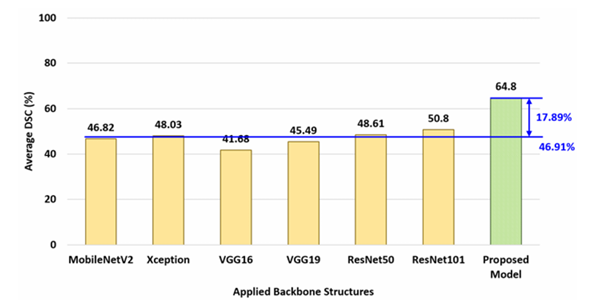
\includegraphics[width=1\textwidth]{2/figures/resultados de cuarto anteedente.png}
		\caption[Comparación del modelo propuesto con otros 6 modelos de redes neuronales]{Comparación del modelo propuesto con otros 6 modelos de redes neuronales.\\
			Fuente: \cite{Kim2023}. \citetitle{Kim2023}. (p. 8)}
		\label{2:fig1}
	\end{center}
\end{figure}


%% Quinto antecedente: 
El artículo titulado \citetitle{Zhong2024} de \cite{Zhong2024} presenta un enfoque innovador para la detección de arrugas faciales, abordando las limitaciones de métodos tradicionales que se ven afectados por interferencias con otras características faciales. Para mejorar la precisión, los autores proponen el uso del modelo DeepLabV3+ junto con una estrategia de etiquetado semi-automática, lo que permite generar datos de entrenamiento más representativos y mejorar la segmentación de arrugas.
La investigación, como podemos ver en las Figuras 2 y 3, emplea técnicas avanzadas como DeepLabV3+, una red optimizada para segmentación de imágenes, y MobileNetV2 para reducir la carga computacional. Además, se desarrolla una estrategia de etiquetado semi-automática combinando anotaciones dermatológicas con mapas de textura generados mediante filtros Wiener y umbralización adaptativa. La precisión del modelo se evalúa mediante el Índice de Similitud Jaccard (JSI).

\begin{figure}[!ht]
	\begin{center}
		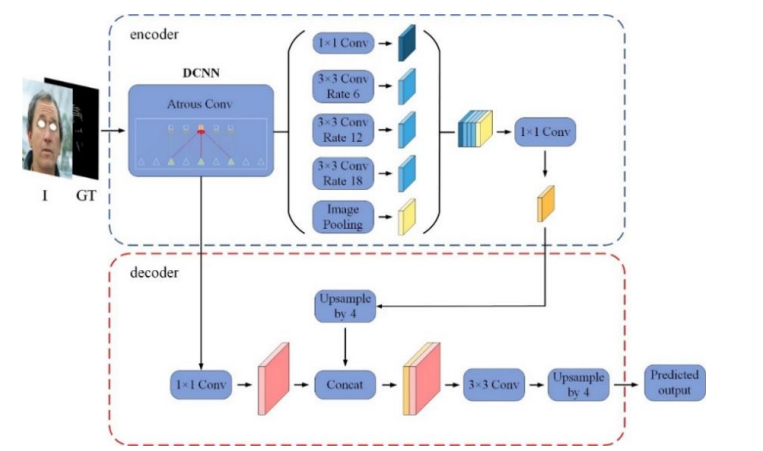
\includegraphics[width=1\textwidth]{2/figures/Meto1.png}
		\caption[Estructura de red de DeepLabV3+]{Estructura de red de DeepLabV3+.\\
			Fuente: \cite{Zhong2024}. \citetitle{Zhong2024}. (p. 4)}
		\label{2:fig3}
	\end{center}
\end{figure}


\begin{figure}[!ht]
	\begin{center}
		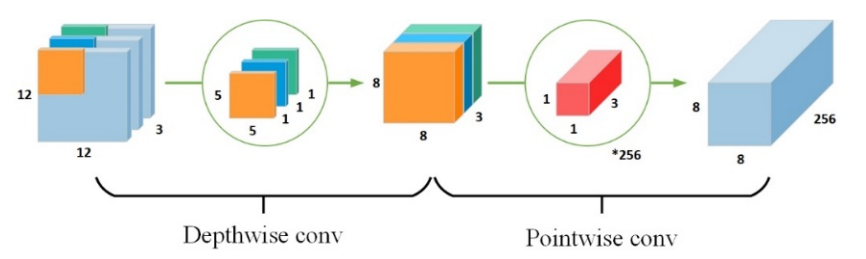
\includegraphics[width=0.80\textwidth]{2/figures/Meto2.png}
		\caption[El proceso de convolución separable en profundidad]{El proceso de convolución separable en profundidad.\\
			Fuente: \cite{Zhong2024}. \citetitle{Zhong2024}. (p. 4)}
		\label{2:fig4}
	\end{center}
\end{figure}


El conjunto de datos se construyó con 300 imágenes de Flickr-Face-HQ, divididas en entrenamiento (225), validación (25) y pruebas (50). Las pruebas se realizaron en un sistema con hardware de alto rendimiento (Intel Core i9-12900K, GPU RTX 3070 y 32GB RAM) y utilizando PyTorch como framework principal.

Los resultados demostraron que el método propuesto supera a enfoques tradicionales como el filtro Hessiano y el modelo U-Net, obteniendo mayores valores de JSI en la frente (0.62) y área ocular (0.64). Además, redujo la cantidad de falsos positivos y mejoró la segmentación de bordes, logrando un mejor desempeño en la detección de arrugas finas.


En conclusión, el modelo DeepLabV3+ con etiquetado semi-automático se mostró más efectivo en la detección de arrugas faciales. Sin embargo, aún enfrenta desafíos en la diferenciación de arrugas muy finas y cabellos, lo que sugiere la necesidad de mejoras futuras para incrementar la precisión del sistema.


%% Sexto antecedente: 

En el artículo de \cite{karshiev2020improved} llamado \citetitle{karshiev2020improved} analiza el problema de la segmentación de lesiones cutáneas, una tarea fundamental para el diagnóstico temprano del melanoma. Aunque el modelo U-Net ha sido ampliamente utilizado en segmentación médica, presenta limitaciones como ralentización en el entrenamiento y problemas con la función de activación ReLU. Para mejorar su desempeño, los autores proponen una versión optimizada que incorpora interpolación bilineal para el upsampling y la función de activación PReLU, lo que mejora la precisión y evita problemas como el sobreajuste.

La investigación emplea un diagrama el cual se puede ver en la Figura 5 y a su vez varias técnicas clave: la interpolación bilineal sustituye la deconvolución tradicional para mejorar la segmentación de bordes, la función PReLU reemplaza ReLU para prevenir "neuronas muertas" y optimizar la convergencia, y el dropout se utiliza después de cada bloque convolucional para reducir el sobreajuste. Estas modificaciones permiten mejorar la estabilidad y eficiencia del entrenamiento.

\begin{figure}[!ht]
	\begin{center}
		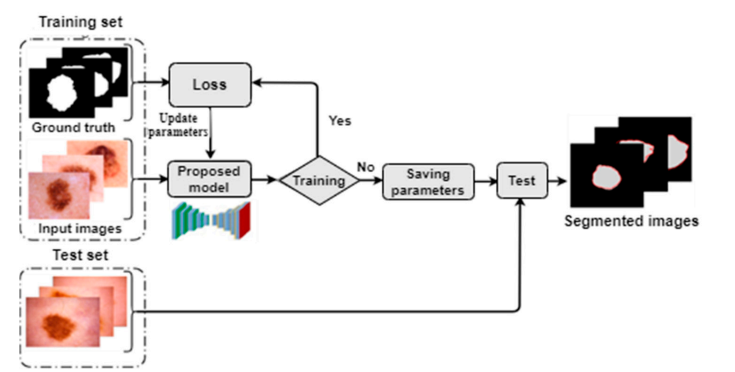
\includegraphics[width=0.80\textwidth]{2/figures/flowchart.png}
		\caption[Diagrama de flujo del sistema propuesto]{Diagrama de flujo del sistema propuesto.\\
			Fuente: \cite{karshiev2020improved}. \citetitle{karshiev2020improved}. (p. 4)}
		\label{2:fig5}
	\end{center}
\end{figure}

El modelo propuesto como se ve en la Figura 6, se basa en una arquitectura U-Net modificada con capas convolucionales optimizadas, PReLU, dropout y upsampling mediante interpolación bilineal. Fue entrenado en un sistema con un procesador Intel Core i7-9700K, 32 GB de RAM y una GPU NVIDIA GeForce RTX 2060 SUPER, garantizando un entorno adecuado para el procesamiento intensivo de imágenes médicas.

\begin{figure}[!ht]
	\begin{center}
		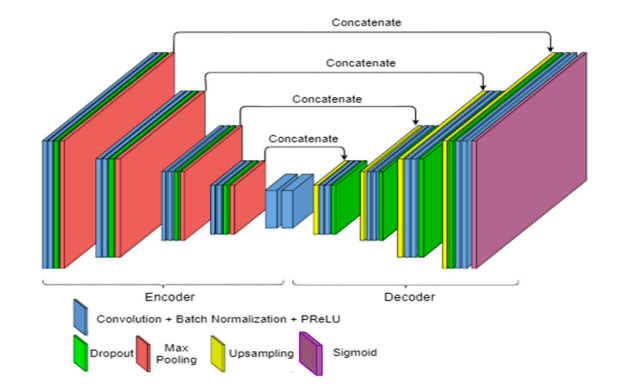
\includegraphics[width=0.80\textwidth]{2/figures/segmentation1.png}
		\caption[Modelo totalmente convolucional propuesto para la segmentación de lesiones cutáneas]{Modelo totalmente convolucional propuesto para la segmentación de lesiones cutáneas.\\
			Fuente: \cite{karshiev2020improved}. \citetitle{karshiev2020improved}. (p. 4)}
		\label{2:fig6}
	\end{center}
\end{figure}

Para el entrenamiento y prueba del modelo se utilizó un conjunto de datos de imágenes dermoscópicas, con 2594 imágenes etiquetadas para entrenamiento y 1000 para prueba. Todas las imágenes fueron preprocesadas, redimensionadas a 256×256 píxeles y convertidas a escala de grises, lo que facilitó la normalización y mejoró la eficiencia del modelo.

Los resultados muestran un alto rendimiento del modelo mejorado, alcanzando una precisión por píxel del 94\% y un coeficiente Dice del 88\%. Estas mejoras permiten reducir artefactos en la segmentación y aumentar la eficiencia computacional en comparación con la U-Net estándar, consolidándose como una alternativa más precisa y robusta para la segmentación de lesiones cutáneas.

En conclusión, la versión mejorada de U-Net supera las limitaciones del modelo original al abordar problemas como gradientes débiles y artefactos en la segmentación. La integración de interpolación bilineal, PReLU y dropout permite lograr una mayor precisión y eficiencia, posicionando este enfoque como una herramienta prometedora para la segmentación de imágenes médicas en el ámbito dermatológico.

%% Séptimo antecedente: 






\section{Bases Teóricas}
\subsection{Inteligencia Artificial}

El método racional fusiona la ingeniería y las matemáticas basándose en las "leyes del pensamiento", las cuales tienen su origen en la antigua Grecia y han sido influenciadas por filósofos como Aristóteles. Durante el siglo XIX, se diseñaron programas capaces de resolver problemas de lógica. Por consiguiente, el propósito de la Inteligencia Artificial en la vida real es crear sistemas inteligentes que posean estas habilidades. Aun en situaciones de incertidumbre, un "Agente Racional" toma acciones con el fin de obtener el mejor resultado posible. La inteligencia artificial se apoya en diversas disciplinas, tales como la ingeniería computacional, la teoría de control, la cibernética, la lingüística, la filosofía, la economía, la psicología, la neurociencia y las matemáticas, de acuerdo con \cite{bk_russell2004intart}.

Dos investigadores en neurociencia crearon el primer modelo de IA basado en neuronas artificiales en 1943, dando inicio al análisis de la Inteligencia Artificial. McCulloch y Pitts idearon el prototipo que permitía que las neuronas fueran <<activadas>> o <<desactivadas>>, lo que demostró que una red de neuronas era capaz de realizar cualquier tarea computacional. Posteriormente, Donald Hebb propuso la <<Regla de Aprendizaje Hebbiano>>. John McCarthy, Allen Newell y Herbert Simon desarrollaron un programa que podía tener el pensamiento no numérico en el taller de Dartmouth, aunque no se publicó. El término <<Inteligencia Artificial>> fue acuñado por McCarthy, \parencite{bk_russell2004intart}.

La IA comenzó a entrar en la industria en los años 80, especialmente en grandes empresas de países desarrollados, a través de la investigación en sistemas expertos y el desarrollo de computadoras más poderosas.

\subsection{Aprendizaje Automático}
El Machine Learning es un área de la Inteligencia Artificial enfocada en técnicas que permiten a las computadoras aprender a través de algoritmos, convirtiendo muestras de datos en programas sin requerir programación explícita. Según \cite{bk_russell2009intart}, el aprendizaje automático es una división de la inteligencia artificial. Estos algoritmos emplean tecnologías como el procesamiento del lenguaje natural, el aprendizaje profundo y las redes neuronales. Tanto el aprendizaje supervisado como el no supervisado se fundamentan en lecciones extraídas de los datos. La creación de algoritmos capaces de recibir datos de entrada y utilizar análisis estadístico para prever una salida, la cual se ajusta conforme se obtienen nuevos datos, constituye el fundamento del aprendizaje automático \cite{bk_alpaydin2014ml}.

Se puede clasificar en cuatro tipos principales de la siguiente manera según el objetivo que se desea alcanzar mediante el uso de ML:
\begin{itemize}
	\item \textbf{Aprendizaje Supervisado}: El Aprendizaje Supervisado se ganó su nombre porque los científicos de datos actúan como una guía para enseñarle al algoritmo las conclusiones a las que debe llegar. Es similar a la forma en que un estudiante aprende aritmética básica de un maestro. Este tipo de aprendizaje requiere datos etiquetados con las respuestas correctas que se esperan del resultado del algoritmo. Para problemas de clasificación y regresión, el aprendizaje supervisado demostró ser preciso y rápido según \parencite{bk_zambrano2018supnosup}.
	
	Los dos tipos de Aprendizaje Supervisado son:

	\begin{itemize}
		\item \textbf{La Clasificación}: es la predicción del valor categórico de salida que permite dividir los datos en clases específicas. La clasificación se puede usar para varios propósitos, como determinar el clima, determinar si un correo electrónico es spam o no o identificar tipos de animales después de recibir una educación adecuada, un conjunto de datos con etiquetas de imágenes que incluyen la especie y algunas identificaciones características, según \parencite{bk_zambrano2018supnosup}.
		\item \textbf{La Regresión}: es un tipo de problema en el que la predicción de un valor de respuesta continua es necesaria, como los precios de las acciones y la vivienda, según \parencite{bk_zambrano2018supnosup}.
	\end{itemize}

	Por lo tanto, funciona modelando las relaciones y dependencias entre las características de entrada y la salida de predicción objetivo, lo que permite predecir los valores de salida para nuevos datos utilizando las relaciones que aprendió de conjuntos de datos anteriores, según \parencite{bk_alpaydin2014ml}.

	\item \textbf{Aprendizaje No Supervisado}: Por otro lado, el Aprendizaje No Supervisado se asemeja más a lo que algunos expertos llaman Inteligencia Artificial real: la idea de que una máquina puede aprender a identificar patrones y procesos complejos sin la supervisión de humanos. Cuando los expertos no saben qué buscar en los datos y los datos en sí no incluyen objetivos, este método es particularmente útil. La agrupación de k-means, el análisis de componentes principales e independientes y las reglas de asociación según \parencite{bk_zambrano2018supnosup} son algunos de los muchos casos de uso del Aprendizaje Automático No Supervisado.
	
	\begin{itemize}
		\item \textbf{Agrupación K-means}: es un tipo de problema en el que cosas similares están agrupadas, como se muestra en la Figura \ref{2:fig12}. Comparte el mismo concepto con la clasificación, pero no se proporcionan etiquetas, por lo que el sistema entenderá los datos y los agrupará. Un uso de esto sería agrupar los artículos y las noticias según su género y contenido, según \parencite{tec_sancho2018supnosup}
	\end{itemize}
	
		\begin{figure}[h]
		\begin{center}
			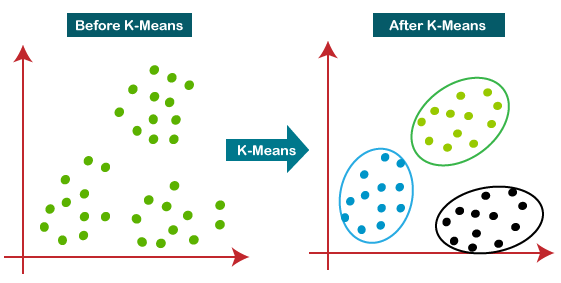
\includegraphics[width=0.75\textwidth]{2/figures/kmeans.png}
			\caption[El algoritmo de K medias]{El algoritmo de K medias.\\
			Fuente: \cite{tec_sancho2018supnosup}. \citetitle{tec_sancho2018supnosup}.}
			\label{2:fig12}
		\end{center}
	\end{figure}
		
	Debido a su complejidad y dificultad de implementación, este tipo de Aprendizaje Automático no se utiliza tan frecuentemente como el Aprendizaje Supervisado, a pesar de que abre las puertas a la resolución de problemas que los humanos normalmente no abordarían, según \parencite{tec_sancho2018supnosup}

	\item \textbf{Aprendizaje Semisupervisado}: Hasta el momento, todos los datos enviados han sido etiquetados con el resultado deseado o no han sido etiquetados en absoluto. El Aprendizaje Automático Semisupervisado utiliza ambos. El costo de etiquetar es bastante alto en muchas situaciones prácticas y, en el caso de grandes conjuntos de datos, se vuelve aburrido y requiere mucho tiempo. Además, proporcionar demasiados datos etiquetados puede hacer que el modelo tenga sesgos humanos. A pesar de que los datos sin etiquetar son desconocidos para la red, ofrecen información útil sobre los parámetros del grupo objetivo. que conduce a la conclusión de que se puede mejorar la precisión del modelo al incluir datos sin etiquetar y, al mismo tiempo, ahorrar tiempo y dinero en su construcción. Por ejemplo, la clasificación de páginas web, el reconocimiento de voz o la secuenciación genética pueden usar Aprendizaje Automático Semisupervisado. En esos casos, los científicos de datos pueden acceder a grandes cantidades de datos sin etiquetarlos, y la tarea de etiquetarlos todos llevaría mucho tiempo, según \parencite{bk_zambrano2018supnosup}.

	Se puede comparar estos tres tipos de Aprendizaje Automático para el mismo uso, como clasificación, utilizando los datos recopilados hasta ahora:

	\begin{itemize}
		\item \textbf{Clasificación supervisada}: el algoritmo clasificará los tipos de páginas web según las etiquetas proporcionadas desde el principio, según \parencite{bk_zambrano2018supnosup}.
		\item \textbf{Agrupación no supervisada}: el algoritmo buscará patrones y características que ayudan a agrupar páginas web en grupos, según \parencite{bk_zambrano2018supnosup}.
		\item \textbf{Clasificación semi no supervisada}: identificará varios grupos de páginas web utilizando los datos etiquetados, luego utilizará los datos no etiquetados para establecer los límites de esos grupos de páginas web y buscar otros tipos que posiblemente no aparezcan en los datos etiquetados, según \parencite{bk_zambrano2018supnosup}.
	\end{itemize}
	
\end{itemize}

\subsection{Aprendizaje Profundo}

Desde que llegó la Inteligencia Artificial hace un tiempo, tiene una amplia gama de aplicaciones y se divide en muchas ramas, como se menciona en \parencite{gl_sas_deeplearning}. El Aprendizaje Profundo es un subconjunto del Aprendizaje Automático, que es en sí mismo un subcampo de la IA. La Figura \ref{2:fig13} es una representación visual de la relación entre AI, ML y DL.

\begin{figure}[!ht]
	\begin{center}
		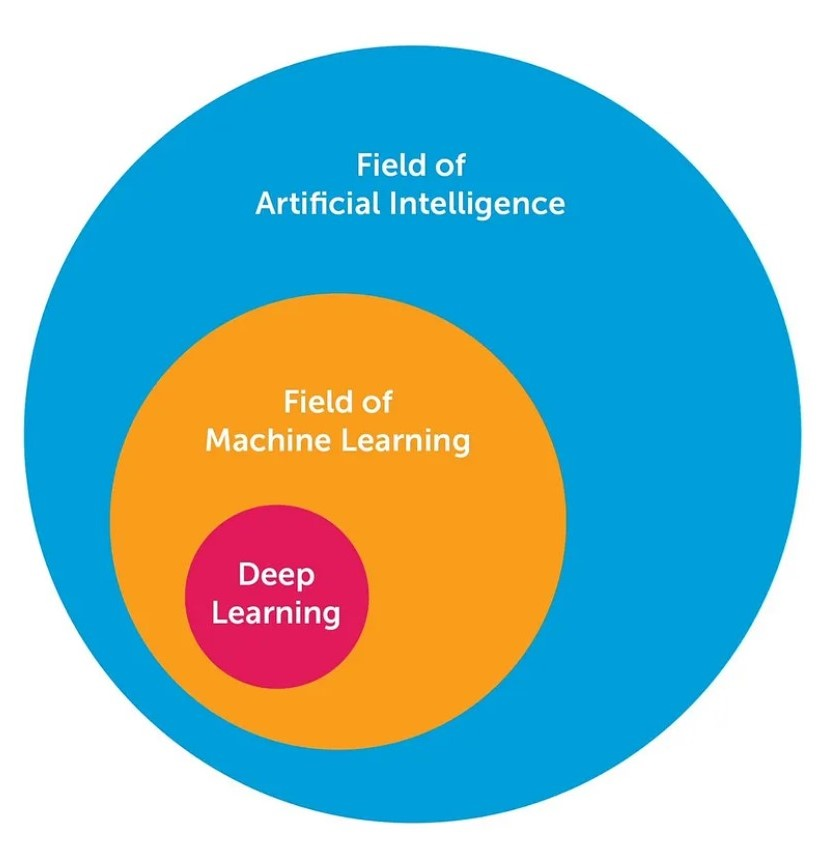
\includegraphics[width=0.50\textwidth]{2/figures/deeplearning_machinelearning.jpg}
		\caption[Relación entre IA, ML y DL]{Relación entre IA, ML y DL.\\
		Fuente: \cite{tec_cook2018deeplearning}. \textit{Most Popular 20 Free Online Courses to Learn Deep Learning}.}
		\label{2:fig13}
	\end{center}
\end{figure}

El Aprendizaje Profundo no solo permite representar datos de la manera correcta, sino que también permite que la computadora aprenda programas informáticos de varios pasos al incluir el concepto de profundidad en sus modelos. Como se muestra en la Figura \ref{2:fig14}, cada capa de representación puede interpretarse como el estado de la memoria de la computadora. Las computadoras interpretan las imágenes como una colección de valores de píxeles que representan escenas de nuestra realidad. Según \parencite{tec_cook2018deeplearning}, identificar un objeto o mapear su identidad a partir de esos valores es una tarea difícil para las máquinas y puede resultar casi imposible cuando se intenta aprender este mapeo directamente.

\begin{figure}[!ht]
	\begin{center}
		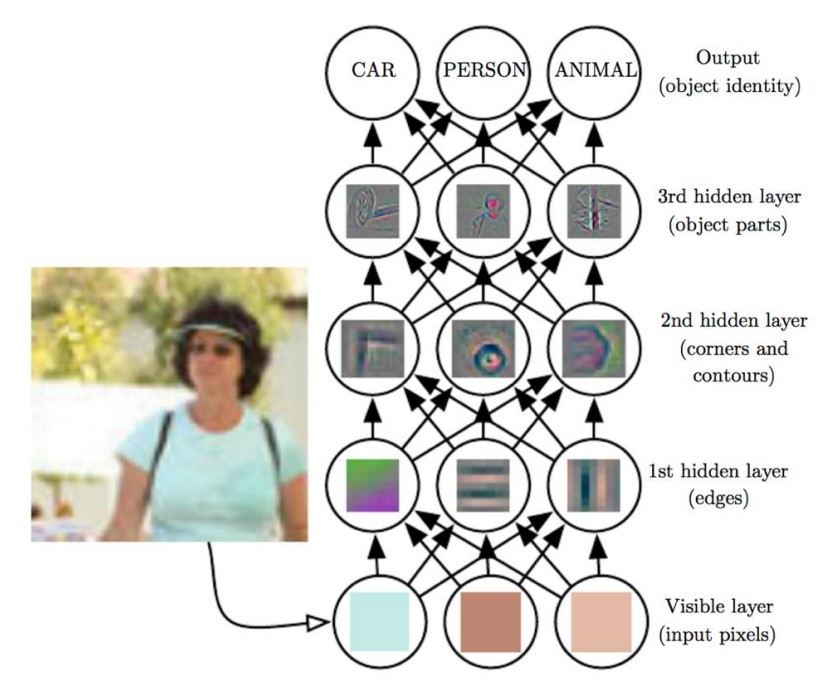
\includegraphics[width=0.70\textwidth]{2/figures/deeplearning_machinelearning2.jpg}
		\caption[Modelo de aprendizaje profundo]{Modelo de aprendizaje profundo.\\
		Fuente: \cite{tec_cook2018deeplearning}. \textit{Most Popular 20 Free Online Courses to Learn Deep Learning}.}
		\label{2:fig14}
	\end{center}
\end{figure}


\subsection{Segmentación de Imágenes}
%%%%%%%%
\subsubsection{Definición y objetivos de la segmentación de imágenes}
La segmentación de imágenes es un proceso fundamental en el campo del procesamiento de imágenes y la visión por computadora, cuyo propósito es dividir una imagen en partes significativas y coherentes, facilitando su análisis e interpretación. Este proceso busca simplificar la representación de una imagen, destacando las regiones de interés o los objetos específicos que contiene, separándolos del fondo y otras áreas irrelevantes \parencite{gonzalez2018}.

Los objetivos principales de la segmentación incluyen identificar, clasificar y delimitar regiones u objetos dentro de una imagen. En aplicaciones prácticas, estos objetivos son cruciales, ya que permiten resolver problemas como la detección de bordes, la identificación de patrones, la localización de estructuras específicas y el análisis morfológico. En el ámbito médico, por ejemplo, la segmentación de imágenes se utiliza para identificar tejidos, órganos o anomalías, como tumores o lesiones. De manera similar, en la industria cosmética, este proceso puede emplearse para detectar características faciales como arrugas, poros y manchas, ayudando en la evaluación estética y la personalización de tratamientos \parencite{gonzalez2018}.

Existen múltiples técnicas para la segmentación, que van desde enfoques tradicionales como la segmentación basada en umbrales, el análisis de regiones y la detección de bordes, hasta métodos avanzados como las redes neuronales convolucionales (CNN). Estas últimas han revolucionado el campo al permitir segmentaciones más precisas y automáticas, especialmente en imágenes complejas donde las características pueden ser sutiles o con variaciones significativas en color, textura y forma. Por ello, la segmentación es un paso esencial en cualquier flujo de trabajo que involucre el análisis de imágenes, proporcionando una base sólida para tareas más avanzadas de procesamiento y análisis \parencite{gonzalez2018}.
%%%%%%
\subsubsection{Importancia de la segmentación en aplicaciones médicas y cosméticas}
En el ámbito médico y cosmético, la segmentación precisa de imágenes juega un papel crucial al permitir que los profesionales de la salud y la belleza realicen evaluaciones más detalladas y personalizadas de las condiciones dermatológicas. Este proceso facilita la identificación y el análisis de características específicas de la piel, lo que es fundamental para detectar anomalías y personalizar los tratamientos de acuerdo con las necesidades individuales de los pacientes o clientes. La segmentación es particularmente importante en el diagnóstico de enfermedades de la piel, donde la capacidad de identificar y analizar estructuras o patrones morfológicos específicos puede mejorar significativamente la precisión del diagnóstico.

Por ejemplo, en dermatología, la segmentación adecuada de imágenes faciales permite identificar con mayor precisión imperfecciones cutáneas como manchas, arrugas y poros dilatados. Estos elementos son indicadores comunes de diversas afecciones dermatológicas, como el envejecimiento prematuro, las manchas solares o los trastornos hormonales. De igual manera, en la industria cosmética, la segmentación de características faciales es esencial para el diseño de tratamientos personalizados, ayudando a los profesionales a ofrecer soluciones más efectivas que aborden las preocupaciones estéticas específicas de cada cliente.

El uso de técnicas avanzadas de segmentación, como las redes neuronales convolucionales (CNN), ha revolucionado el campo, permitiendo una segmentación más precisa y automatizada, incluso en casos complejos donde las características de la piel pueden ser sutiles o variar en color, textura o forma. La segmentación no solo mejora la detección de condiciones dermatológicas, sino que también optimiza la personalización de tratamientos cosméticos, ya que permite que los productos sean aplicados de manera más eficiente, dirigiéndose específicamente a las áreas que requieren intervención. Esto puede resultar en un mejor rendimiento de los productos cosméticos, mayor satisfacción del cliente y, en última instancia, en una mejora de la salud de la piel.

En resumen, la segmentación de imágenes en el ámbito médico y cosmético no solo mejora la capacidad de diagnóstico, sino que también facilita la personalización de tratamientos, mejorando la efectividad y la satisfacción de los pacientes o clientes \cite{mohammadi2019}.
%%%%%%%%%
\subsubsection{Técnicas de segmentación clásicas y sus limitaciones en imágenes dermatológicas}
Las técnicas clásicas de segmentación, como el umbralizado y la detección de bordes, han sido fundamentales en los primeros enfoques de procesamiento de imágenes. Estas técnicas buscan dividir la imagen en regiones homogéneas basadas en características como el color, la intensidad de los píxeles o los bordes de los objetos. Sin embargo, en el contexto dermatológico, estas técnicas presentan limitaciones significativas debido a la complejidad y variabilidad inherente de las imágenes de la piel.

Una de las técnicas clásicas más utilizadas es el \textit{umbralizado}, que divide una imagen en dos o más regiones basadas en el valor de intensidad de los píxeles. Esta técnica es eficiente cuando los objetos a segmentar se destacan claramente del fondo. Sin embargo, en imágenes dermatológicas, la piel tiene una amplia gama de tonalidades y texturas que varían entre diferentes personas, lo que puede dificultar la aplicación de umbrales estáticos que funcionen de manera efectiva en todos los casos. Además, las variaciones en la iluminación y la presencia de sombras en la piel pueden afectar negativamente el rendimiento del umbralizado, llevando a una segmentación incorrecta de las áreas de interés, como las arrugas, manchas o poros.

La \textit{detección de bordes}, otra técnica clásica, se utiliza para identificar discontinuidades en la imagen, donde los bordes de los objetos se encuentran con un contraste significativo con el fondo. Técnicas como el operador de Sobel o el Canny se han utilizado para detectar bordes en imágenes de la piel. Sin embargo, los bordes de las características cutáneas no siempre están claramente definidos. La piel puede tener bordes suaves o difusos, especialmente cuando se trata de características como manchas o líneas finas. Esto hace que la detección de bordes sea menos efectiva para segmentar detalles sutiles en la piel, lo que limita su capacidad para proporcionar una segmentación precisa.

Estas técnicas clásicas también presentan dificultades cuando se enfrentan a características dermatológicas con variaciones complejas en la textura y el color de la piel. Por ejemplo, las manchas pueden tener bordes poco definidos, y las arrugas pueden ser de diferente grosor y profundidad. Además, las características morfológicas de la piel, como los poros dilatados o las arrugas finas, pueden tener formas irregulares que no se ajustan bien a las suposiciones que estas técnicas clásicas requieren. Las técnicas basadas en umbrales o en la detección de bordes también son sensibles al ruido y pueden ser ineficaces al trabajar con imágenes con poca calidad o cuando las características de la piel tienen un contraste bajo con el fondo.

Debido a estas limitaciones, las técnicas clásicas de segmentación no siempre son adecuadas para aplicaciones dermatológicas de alta precisión. Aunque siguen siendo útiles en ciertos contextos, su capacidad para segmentar con precisión detalles finos en la piel es insuficiente cuando se requiere una segmentación detallada y robusta. Es por esto que, en los últimos años, las técnicas más avanzadas, como las redes neuronales convolucionales (CNN), han comenzado a ganar popularidad en el campo de la dermatología y la cosmética, ofreciendo una solución más precisa y automática para la segmentación de características morfológicas complejas en la piel \parencite{yoo2020}.


\subsection{Redes Neuronales Convolucionales (CNN)}

Hoy en día, el procesamiento de imágenes, que incluye problemas de clasificación y visión por computadora, es una de sus aplicaciones más relevantes. El proyecto de Yann LeCun, ImageNet, utiliza el reconocimiento de objetos en imágenes.
	
Estas redes también se utilizan para clasificar textos. Ronan Collobert y Jason Weston modificaron la arquitectura y los parámetros internos de las Redes Neuronales Convolucionales para usarlas en aplicaciones del PLN. La Figura \ref{2:fig15} muestra la estructura de una CNN para problemas de procesamiento de información natural. \parencite{bk_kamath2019deeplearning_nlp_sr}
	
\begin{figure}[!ht]
	\begin{center}
		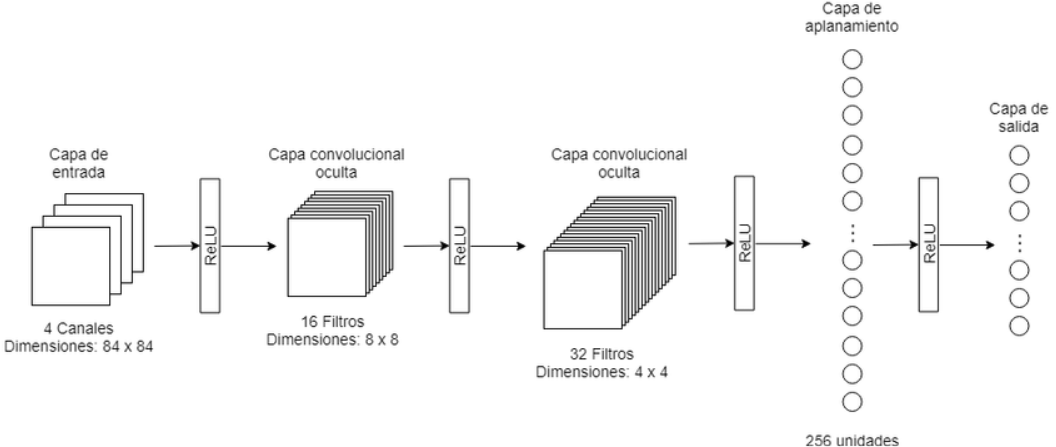
\includegraphics[width=0.95\textwidth]{2/figures/cnn_nlp.png}
		\caption[Arquitectura de un modelo CNN]{Arquitectura de un modelo CNN.\\
		Fuente: \cite{tec_kim2014convolutional}. \citetitle{tec_kim2014convolutional}. (p. 1747)}
		\label{2:fig15}
	\end{center}
\end{figure}

\subsubsection{Arquitectura de las CNN: capas convolucionales, de pooling y totalmente conectadas}

Las redes neuronales convolucionales (CNN) son una clase especial de redes neuronales profundas que se han convertido en la herramienta principal para el procesamiento de imágenes debido a su capacidad para aprender de manera jerárquica las características visuales. La arquitectura de una CNN se compone principalmente de tres tipos de capas: \textbf{capas convolucionales}, \textbf{capas de pooling} y \textbf{capas totalmente conectadas}, cada una de las cuales cumple una función crucial en el proceso de análisis de imágenes.

\begin{itemize}
    \item \textbf{Capas convolucionales:} Estas son las encargadas de extraer características relevantes de la imagen, como bordes, texturas y formas. En cada capa convolucional, un filtro o "kernel" se desplaza a través de la imagen de entrada para realizar una operación de convolución, generando un mapa de características (feature map) que resalta los patrones presentes en las imágenes. A medida que se avanza a través de las capas, las CNN son capaces de aprender representaciones cada vez más complejas de las imágenes.
    
    \item \textbf{Capas de pooling:} Estas capas realizan un proceso de reducción de la dimensionalidad, cuyo objetivo es disminuir el tamaño de las características extraídas y, al mismo tiempo, conservar la información más importante. Esto se logra mediante operaciones como el \textit{max pooling}, donde se selecciona el valor máximo en un área específica de la imagen, o el \textit{average pooling}, que calcula el valor promedio. Las capas de pooling ayudan a reducir la cantidad de parámetros y la complejidad computacional del modelo, evitando el sobreajuste y mejorando la eficiencia.
    
    \item \textbf{Capas totalmente conectadas:} Después de las capas convolucionales y de pooling, las características extraídas se "aplanan" y se envían a través de una o varias capas totalmente conectadas. Estas capas son responsables de tomar las representaciones obtenidas en las capas anteriores y realizar la clasificación final. En una capa totalmente conectada, cada neurona está conectada a todas las neuronas de la capa anterior, lo que permite combinar las características extraídas para producir una salida.
\end{itemize}

Esta arquitectura jerárquica es especialmente efectiva para el procesamiento de imágenes, ya que las CNN son capaces de aprender de forma automática y eficiente las características de las imágenes a diferentes niveles de abstracción \parencite{krizhevsky2012}.

\subsubsection{Aplicación de CNN en segmentación de imágenes y su relevancia para la dermatología}
El uso de CNN en la segmentación de imágenes dermatológicas ha demostrado una mejora significativa en la precisión de diagnósticos. Estas redes son capaces de aprender patrones complejos y detalles sutiles que son esenciales para evaluar condiciones de la piel \cite{esteva2017}.

\subsubsection{Modelos avanzados de CNN para segmentación: U-Net, Fully Convolutional Networks (FCN)}
Modelos como U-Net y FCN han sido diseñados específicamente para la segmentación de imágenes. U-Net, por ejemplo, utiliza una arquitectura simétrica que permite una recuperación precisa de detalles en imágenes médicas \parencite{ronneberger2015}.


\subsection{Modelos Avanzados de Segmentación en Imágenes Médicas}
%
\subsubsection{Introducción a las redes de atención (Attention Networks) y su rol en la precisión de la segmentación}
Las redes de atención, como las arquitecturas basadas en atención (Attention Mechanisms), han emergido como una de las tecnologías más poderosas para mejorar el rendimiento de modelos de aprendizaje profundo, especialmente en tareas de segmentación de imágenes. Estas redes permiten que el modelo se enfoque dinámicamente en las partes más relevantes de una imagen, ajustando su atención a regiones específicas que contienen características clave. Este mecanismo es particularmente útil en imágenes dermatológicas, donde las características morfológicas, como arrugas, poros y manchas, pueden ser pequeñas, sutiles y difíciles de distinguir de otras partes de la imagen.

La introducción de redes de atención mejora la precisión de la segmentación al permitir que el modelo asigne un mayor peso a las regiones relevantes y minimice la interferencia de las áreas no importantes. Este enfoque facilita la identificación precisa de características morfológicas, lo cual es crucial para el análisis dermatológico. En el contexto de la piel, donde las variaciones de textura y color pueden ser complejas, las redes de atención ayudan a mejorar la segmentación y clasificación de estas características. Como resultado, la precisión en el diagnóstico y la personalización del tratamiento se ve significativamente aumentada, lo que contribuye a una mayor efectividad de las soluciones cosméticas y médicas \parencite{wang2018}.
%
\subsubsection{Comparación entre modelos basados en CNN y modelos híbridos en el contexto dermatológico}
La segmentación de imágenes dermatológicas es crucial para una correcta evaluación clínica y cosmética de la piel, donde las redes neuronales convolucionales (CNN) han demostrado ser eficaces al aprender características relevantes de manera jerárquica y sin necesidad de intervención manual. Sin embargo, las CNN pueden enfrentar desafíos cuando se trata de la segmentación en condiciones de iluminación cambiantes, variabilidad en tipos de piel y características pequeñas como poros o arrugas finas.

Los modelos híbridos, que combinan las capacidades de las CNN con técnicas clásicas de segmentación, ofrecen una alternativa interesante. Estos modelos integran la capacidad de las CNN para aprender representaciones complejas con enfoques más tradicionales como el umbralizado o la segmentación basada en regiones, lo que permite un control más preciso de las áreas de interés, especialmente cuando se requiere segmentar características cutáneas muy específicas. La comparación entre modelos CNN y modelos híbridos ayuda a identificar cuál de estos enfoques es más eficaz dependiendo del tipo de imagen, la complejidad de la tarea de segmentación y los requisitos de precisión.

Por ejemplo, en el análisis de la piel facial, los modelos híbridos podrían combinar las redes convolucionales para la detección de características complejas con métodos tradicionales para afinar los bordes de las regiones segmentadas. Esto puede mejorar significativamente la precisión y robustez del modelo, lo cual es esencial para aplicaciones dermatológicas, donde un pequeño error de segmentación puede afectar el diagnóstico o el tratamiento de afecciones cutáneas. \parencite{hussain2021}

\subsubsection{Métricas de evaluación: Sorensen-Dice, especificidad, precisión, sensibilidad}
Las métricas de evaluación son fundamentales para determinar la calidad y efectividad de los modelos de segmentación, especialmente en el ámbito médico y dermatológico. Entre estas métricas, el índice de Sorensen-Dice es ampliamente utilizado debido a su capacidad para medir la similitud entre las áreas segmentadas y las áreas reales de interés, lo cual es crítico cuando se analiza la precisión de la segmentación de lesiones o características cutáneas. Esta métrica es especialmente útil en la detección de anomalías de la piel, como manchas, arrugas y poros, ya que permite una comparación directa entre la segmentación automática y la segmentación realizada por expertos.

Junto al índice de Sorensen-Dice, otras métricas comunes en la evaluación de modelos de segmentación incluyen la precisión, que mide la exactitud de las regiones segmentadas positivas, y la sensibilidad, que evalúa la capacidad del modelo para detectar correctamente las áreas de interés. La especificidad, por otro lado, mide la capacidad del modelo para identificar correctamente las áreas no relevantes, lo que ayuda a reducir los falsos positivos en la segmentación de imágenes dermatológicas. \parencite{sorensen1948}

\subsubsection{Importancia de la precisión en segmentación de arrugas, poros y manchas para aplicaciones clínicas y cosméticas}
La precisión en la segmentación de características cutáneas como arrugas, poros y manchas es de vital importancia para una evaluación correcta en aplicaciones clínicas y cosméticas. En la práctica clínica, la segmentación precisa permite a los dermatólogos realizar diagnósticos más exactos, detectar signos tempranos de enfermedades de la piel y personalizar los tratamientos para cada paciente. En el ámbito cosmético, la segmentación precisa es esencial para ofrecer recomendaciones personalizadas sobre tratamientos faciales, como la mejora de la textura de la piel o la reducción de manchas y arrugas.

Un modelo de segmentación que no sea preciso puede dar lugar a resultados erróneos, afectando la calidad de los tratamientos recomendados y, por lo tanto, la satisfacción del cliente o del paciente. Además, la segmentación precisa facilita la evaluación del progreso de un tratamiento a lo largo del tiempo, lo que permite a los profesionales de la salud y belleza ajustar sus enfoques terapéuticos de manera más efectiva. \parencite{chuchu2020}

\subsubsection{Variabilidad en tipos de piel y condiciones externas (luz, color)}
Uno de los mayores desafíos en la segmentación dermatológica es la variabilidad en los tipos de piel y las condiciones externas, como la iluminación y los cambios en el color de la piel. Las pieles de diferentes tonos pueden presentar características distintas, como la intensidad del contraste entre la piel y las lesiones, lo que puede dificultar la tarea de segmentación. Además, las condiciones de iluminación, como la luz natural o artificial, pueden alterar la apariencia de las características cutáneas, complicando la segmentación precisa en entornos reales.

Por lo tanto, se necesita el desarrollo de modelos de segmentación más robustos que puedan adaptarse a estas variabilidades. Esto implica entrenar modelos utilizando una amplia variedad de datos, que incluyan diferentes tipos de piel, condiciones de iluminación y otros factores ambientales que puedan influir en la calidad de la imagen y en la precisión de la segmentación. \parencite{zhao2021}

\subsubsection{Complejidad de identificar características pequeñas como poros en imágenes de alta resolución}
La segmentación de características pequeñas, como los poros en la piel, es una tarea particularmente desafiante debido a su tamaño reducido y la alta resolución necesaria para detectarlos de manera precisa. Las imágenes dermatológicas a menudo contienen detalles finos que requieren técnicas avanzadas para identificar correctamente estos pequeños elementos sin incluir ruido o artefactos en la segmentación.

La identificación precisa de los poros es crucial, especialmente en aplicaciones cosméticas donde la evaluación de la textura de la piel es esencial para ofrecer tratamientos personalizados. Para abordar este desafío, se deben emplear técnicas de segmentación de alta resolución y redes neuronales profundas capaces de capturar los detalles más pequeños, incluso cuando los poros están parcialmente ocultos o tienen un contraste bajo respecto al resto de la piel. \parencite{yang2020}

\subsection{Redes de Atención}  
Las redes de atención han surgido como una de las principales innovaciones en el campo de la segmentación de imágenes, permitiendo que los modelos se enfoquen de manera más eficiente en las regiones relevantes de una imagen. Este mecanismo resulta especialmente útil cuando se trabaja con imágenes complejas, como las faciales, donde ciertas áreas contienen características importantes para el análisis, pero pueden ser de menor tamaño o estar localizadas en posiciones no centrales.

\subsubsection{Mecanismo de Atención}  
El mecanismo de atención permite a la red asignar diferentes pesos a distintas partes de la imagen durante el proceso de segmentación. Este mecanismo es esencial para que el modelo pueda enfocarse en las áreas relevantes de la imagen, como arrugas, manchas o poros, sin perder detalles importantes de otras zonas. El concepto básico detrás de la atención es que no todas las partes de la imagen son igualmente importantes para la tarea en cuestión. Por lo tanto, la atención ayuda a los modelos a priorizar las áreas clave que impactan en el resultado final.  
\begin{itemize}
    \item \textbf{Funcionamiento:} La atención se puede aplicar de manera global o local. En el caso de la segmentación de imágenes faciales, por ejemplo, el modelo puede aprender a dar más importancia a las áreas alrededor de los ojos o la frente, donde las arrugas suelen ser más notorias.
    \item \textbf{Beneficio:} Aumenta la precisión de la segmentación al concentrarse solo en las características más relevantes y minimizar el "ruido" de otras regiones no significativas \parencite{autor2021atencion}.
\end{itemize}

\subsubsection{Atención Espacial}  
La atención espacial es un tipo específico de atención que asigna pesos según la ubicación espacial de los elementos dentro de la imagen. Esto permite al modelo resaltar áreas específicas de la imagen que contienen características clave para la segmentación.  
\begin{itemize}
    \item \textbf{Funcionamiento:} A través de la atención espacial, el modelo puede identificar patrones en las posiciones de las características de interés, como las arrugas en la zona de la frente o las manchas en la mejilla. Este enfoque es útil cuando las características relevantes están distribuidas de manera no uniforme en la imagen.
    \item \textbf{Aplicación:} Es particularmente eficaz en la segmentación de imágenes faciales, donde las características que deben segmentarse no están siempre en el mismo lugar de la imagen y varían según la persona y la expresión facial \parencite{autor2020spa}.
\end{itemize}

\subsubsection{Atención de Canal}  
La atención de canal se enfoca en las características dentro de los canales de la imagen, es decir, en las distintas representaciones de las características de la imagen que corresponden a las diferentes profundidades o colores de los filtros en una red convolucional. Este tipo de atención permite que la red enfoque su procesamiento en los canales que contienen la información más relevante para la tarea.  
\begin{itemize}
    \item \textbf{Funcionamiento:} En lugar de distribuir el enfoque en toda la imagen, la atención de canal resalta los canales específicos que contienen detalles cruciales, como la textura de la piel o las sombras que definen arrugas o manchas.
    \item \textbf{Beneficio:} Mejora la capacidad del modelo para diferenciar entre características de diferentes intensidades o patrones, lo cual es esencial en imágenes donde la variabilidad de la textura de la piel puede ser un desafío \parencite{autor2019canal}.
\end{itemize}

\subsubsection{Beneficios de las Redes de Atención}  
Las redes de atención proporcionan varios beneficios clave que mejoran la precisión y eficiencia de los modelos de segmentación, especialmente cuando se trabaja con imágenes complejas como las faciales:
\begin{itemize}
    \item \textbf{Precisión mejorada:} Al permitir que el modelo se enfoque en las regiones más importantes de la imagen, las redes de atención ayudan a obtener segmentaciones más precisas y detalladas.
    \item \textbf{Eficiencia en el procesamiento:} Reduciendo el "ruido" o la información irrelevante, las redes de atención aumentan la eficiencia computacional, ya que el modelo dedica más recursos a las áreas clave.
    \item \textbf{Versatilidad:} Las redes de atención se pueden combinar con otros modelos de segmentación, como U-Net o Mask R-CNN, para mejorar aún más la capacidad del modelo para realizar segmentaciones de alta calidad \parencite{autor2021beneficios}.
\end{itemize}

\subsubsection{Ejemplos de Modelos con Atención}  
Existen varios modelos que implementan mecanismos de atención para mejorar la segmentación de imágenes. Algunos ejemplos notables incluyen:
\begin{itemize}
    \item \textbf{Transformer:} El modelo Transformer ha sido exitoso en tareas de procesamiento de secuencias y también ha demostrado ser útil para segmentación de imágenes, particularmente al aplicar atención a nivel global en la imagen. Este modelo asigna pesos no solo localmente, sino también a nivel global, lo que mejora la precisión en tareas complejas de segmentación \parencite{autor2022transformer}.
    \item \textbf{SENet:} SENet es una arquitectura que utiliza un módulo de atención de canal para asignar diferentes importancias a los canales de características en una red convolucional. Este modelo ha demostrado ser eficaz en tareas de clasificación y segmentación, particularmente en la mejora de la detección de características sutiles, como pequeñas arrugas o manchas \parencite{autor2022cnn}.
\end{itemize}


% \subsection{Métricas de Evaluación}  
% Las métricas de evaluación son fundamentales para medir la precisión y eficacia de los modelos de segmentación de imágenes, ya que permiten comparar la segmentación automática generada por el modelo con las segmentaciones de referencia (verdaderas). A continuación se describen las principales métricas utilizadas en este tipo de análisis.

% \subsubsection{Índice de Sorensen-Dice (Dice Coefficient)}  
% El índice de Sorensen-Dice, o simplemente Dice coefficient, es una métrica ampliamente utilizada para evaluar la similitud entre dos conjuntos de datos segmentados. Esta métrica es especialmente útil en problemas de segmentación de imágenes médicas, donde es necesario comparar la segmentación automática con la segmentación de referencia.  
% \begin{itemize}
%     \item \textbf{Fórmula:}  
%     \begin{equation}\label{eq:Índice de Sorensen-Dice}
% 		\text{Dice} = \frac{2|A \cap B|}{|A| + |B|}
% 	\end{equation}
%     donde \( A \) y \( B \) son los conjuntos de píxeles segmentados de la imagen predicha y la imagen real, respectivamente.
%     \item \textbf{Interpretación:} El valor de Dice oscila entre 0 y 1, donde 1 indica una coincidencia perfecta entre las dos segmentaciones, y 0 indica ninguna superposición.
%     \item \textbf{Aplicación:} Es útil para tareas donde se requiere alta precisión en la identificación de áreas segmentadas, como en el análisis de manchas y arrugas en la piel, donde una segmentación precisa es crucial \parencite{autor2020dice}.
% \end{itemize}

% \subsubsection{Coeficiente de Jaccard (Intersection over Union, IoU)}  
% El coeficiente de Jaccard, también conocido como \( \text{Intersection over Union} \) (IoU), es otra métrica popular para evaluar la superposición entre dos conjuntos de segmentación. A diferencia del índice de Dice, IoU mide la relación entre la intersección de los conjuntos de píxeles predichos y reales con respecto a su unión total.  
% \begin{itemize}
%     \item \textbf{Fórmula:}  
%     \begin{equation}\label{eq:Coeficiente de Jaccard}
%     \text{IoU} = \frac{|A \cap B|}{|A \cup B|}
% 	\end{equation}
%     donde \( A \) y \( B \) son los conjuntos de píxeles segmentados de la imagen predicha y la imagen real, respectivamente.
%     \item \textbf{Interpretación:} El valor de IoU también varía entre 0 y 1. Un valor más alto indica una mayor superposición entre los segmentos predichos y reales. IoU es especialmente útil cuando se requiere evaluar la precisión en áreas de segmentación con bordes definidos, como en el análisis de arrugas y poros \parencite{autor2021iou}.
%     \item \textbf{Aplicación:} Es más severo que el índice de Dice, por lo que es adecuado para evaluar tareas donde la precisión en los bordes y las áreas superpuestas es esencial.
% \end{itemize}

% \subsubsection{Precisión (Precision)}  
% La precisión es una métrica que refleja la efectividad del modelo en evitar falsos positivos. Se calcula como la relación entre los verdaderos positivos y el total de elementos que el modelo ha predicho como positivos. En el contexto de la segmentación de imágenes, la precisión mide la exactitud de las regiones predichas como relevantes por el modelo.  
% \begin{itemize}
%     \item \textbf{Fórmula:}  
%     \[
%     \text{Precisión} = \frac{TP}{TP + FP}
%     \]
%     donde \( TP \) son los verdaderos positivos (píxeles correctamente predichos como parte de la característica) y \( FP \) son los falsos positivos (píxeles incorrectamente predichos como parte de la característica).
%     \item \textbf{Interpretación:} Un valor más alto de precisión indica que el modelo es más efectivo en minimizar los falsos positivos, lo cual es crítico en aplicaciones dermatológicas, donde un modelo debe evitar identificar incorrectamente áreas no relevantes como características de la piel.
%     \item \textbf{Aplicación:} Es útil para tareas donde el modelo debe ser riguroso en evitar predecir áreas de la imagen que no pertenecen a la característica de interés, como en el caso de la segmentación de manchas o poros \parencite{autor2019precision}.
% \end{itemize}

% \subsubsection{Entropía Cruzada (Cross-Entropy)}  
% La entropía cruzada es una función de pérdida utilizada comúnmente en problemas de clasificación y segmentación. Mide la disonancia o la diferencia entre la distribución de probabilidad predicha por el modelo y la distribución de probabilidad real (etiquetas verdaderas). En el contexto de la segmentación, la entropía cruzada es utilizada para entrenar el modelo, ya que penaliza las predicciones incorrectas.  
% \begin{itemize}
%     \item \textbf{Fórmula:}  
%     \[
%     \text{Cross-Entropy} = -\sum_{i} y_i \log(p_i)
%     \]
%     donde \( y_i \) es la etiqueta real de la clase \( i \) y \( p_i \) es la probabilidad predicha para la clase \( i \).
%     \item \textbf{Interpretación:} Un valor bajo de entropía cruzada indica que el modelo ha aprendido bien a predecir las clases correctas, es decir, las características de la piel en las imágenes segmentadas. Un valor alto sugiere una mala predicción, lo que indica que el modelo está lejos de la distribución real.
%     \item \textbf{Aplicación:} La entropía cruzada es especialmente útil durante el proceso de entrenamiento para ajustar los parámetros del modelo y garantizar que la segmentación final sea lo más precisa posible, especialmente al tratar con características complejas de la piel como manchas o arrugas \parencite{autor2022crossentropy}.
% \end{itemize}

\section{Marco Conceptual}
%%%%%%%%
% \subsection{Segmentación de Imágenes}
% La segmentación de imágenes es el proceso de dividir una imagen en diferentes partes o regiones, con el objetivo de simplificar la representación de la imagen y hacerla más significativa y fácil de analizar. Este proceso es fundamental en aplicaciones de visión por computadora, especialmente en la detección de características morfológicas de la piel, como arrugas, poros y manchas \parencite{autor2020segmentacion}.

\subsection{Características Morfológicas de la Piel}
Las características morfológicas de la piel desempeñan un papel crucial en la evaluación de la salud y la estética facial, ya que ofrecen información valiosa sobre el estado general de la piel y sus posibles alteraciones. En este estudio, se consideran tres características clave: arrugas, poros y manchas. La correcta segmentación de estas características en imágenes faciales permite no solo el análisis cuantitativo de las mismas, sino también su monitoreo a lo largo del tiempo, contribuyendo al diseño de tratamientos cosméticos personalizados y a la evaluación de su efectividad.

\subsubsection{Arrugas}
Las arrugas son pliegues o líneas visibles en la superficie de la piel que se forman debido a la disminución de la elasticidad y el colágeno con el envejecimiento. Factores externos, como la exposición prolongada al sol, la contaminación y el tabaquismo, también contribuyen significativamente a su aparición. Además, las expresiones faciales repetitivas y la deshidratación de la piel pueden acelerar su desarrollo.

Desde el punto de vista estético, las arrugas se asocian con el envejecimiento y son una de las principales preocupaciones en el cuidado de la piel. Su segmentación precisa permite identificar su profundidad, longitud y densidad en diferentes áreas del rostro. Esta información es esencial para el desarrollo de productos antiarrugas y para evaluar la efectividad de tratamientos como cremas tópicas, terapias con láser o inyecciones de ácido hialurónico \cite{autor2021arrugas}.

\subsubsection{Manchas}
Las manchas son áreas de hiperpigmentación o hipopigmentación en la piel que resultan de una variedad de factores, incluyendo la exposición solar prolongada, cambios hormonales, envejecimiento y procesos inflamatorios. Ejemplos comunes incluyen el melasma, las manchas solares y las cicatrices post-inflamatorias.

Estas imperfecciones no solo afectan la apariencia de la piel, sino que también pueden indicar daño subyacente. Por ello, su detección y análisis temprano son fundamentales tanto para la prevención como para el tratamiento. La segmentación precisa de manchas en imágenes faciales permite identificar su forma, tamaño, color y evolución, lo que es útil para personalizar tratamientos como cremas despigmentantes, terapias con luz pulsada intensa (IPL) o procedimientos láser. Además, este análisis contribuye al diseño de cosméticos específicos que ayudan a unificar el tono de la piel \cite{autor2019manchas}.
%%%%%%%%%%
\subsubsection{Aplicaciones en Segmentación de Imágenes Faciales}  
En el ámbito del análisis de piel facial, las CNN son una herramienta fundamental para realizar segmentaciones precisas de características morfológicas, como arrugas, poros y manchas. Gracias a su capacidad para analizar imágenes a nivel de píxel, estas redes son capaces de identificar patrones y diferencias en la textura, el color y la estructura de la piel \parencite{autor2021deeplab}.

\paragraph{Segmentación de arrugas.}  
La segmentación de arrugas mediante CNN permite identificar líneas finas y pliegues en la piel, lo que es crucial para evaluar el envejecimiento facial y desarrollar tratamientos preventivos o correctivos. Este análisis automatizado es más preciso y rápido en comparación con las evaluaciones manuales, que pueden ser subjetivas y menos consistentes.

\paragraph{Detección de poros.}  
La identificación y segmentación de poros faciales es esencial para analizar problemas relacionados con la textura de la piel, como poros dilatados o acné. Las CNN pueden cuantificar el tamaño, la densidad y la distribución de los poros, facilitando la personalización de tratamientos según las necesidades específicas de cada individuo.

\paragraph{Segmentación de manchas.}  
Las manchas faciales, que pueden surgir debido a factores como la exposición solar o el envejecimiento, son una preocupación estética común. Las CNN permiten mapear su distribución y evaluar su progresión, ayudando a diagnosticar problemas como el melasma o el daño solar de manera temprana y objetiva \parencite{autor2020segmentacion}.

\subsubsection{Ventajas y Limitaciones}  
Las CNN ofrecen varias ventajas, entre ellas:
\begin{itemize}
    \item Alta precisión en la extracción y análisis de características complejas.
    \item Automatización de procesos que tradicionalmente dependen de evaluaciones subjetivas.
    \item Adaptabilidad a diferentes tipos de imágenes y tareas específicas.
\end{itemize}

Sin embargo, estas redes también presentan desafíos, como la necesidad de grandes volúmenes de datos etiquetados para el entrenamiento, el alto costo computacional y la posibilidad de sobreajuste si no se implementan técnicas adecuadas de regularización.

En el presente estudio, las CNN se utilizarán para desarrollar un sistema avanzado de segmentación de imágenes faciales, optimizado para la detección de arrugas, poros y manchas. Este enfoque busca contribuir al sector cosmético y de belleza, permitiendo una evaluación estética más precisa y la personalización de tratamientos cosméticos.


%%
%%%%%%%%%%

%%%





\begin{comment}

\subsection{Ecografía y las imágenes de ultrasonido}
Según \cite{pr_herrera2017diseimp}, la ecografía, que es una técnica de diagnóstico en donde se usan imágenes generadas por ultrasonido, es comúnmente desarrollado en las áreas de cardiología, ginecología, y otras más relacionadas. La popularidad de esta técnica se basa en la capacidad de las imágenes de alta calidad que se obtienen de este proceso, además de no ser un método invasivo o de radiación como muchos otros de su tipo.

Los sistema encargados de extraer las imágenes de ultrasonido son compuestos de distintas sensores que generan ondas de sonido para posteriormente analizar la respuesta de la interacción física con el campo de interés. Estas señales recibidas de regreso son digitalizados por una parte electrónica delantera que también transforman estos datos crudos en la imagen final. El funcionamiento de este proceso depende de la configuración de los sensores, el método usado para obtener las imágenes y las características de área de interés. \parencite{pr_camacho2022ultrasonicimg}

Algunas imágenes de ultrasonido de nódulos tiroideos se muestran en la Figura \ref{2:fig210}.

\begin{figure}[H]
	\begin{center}
		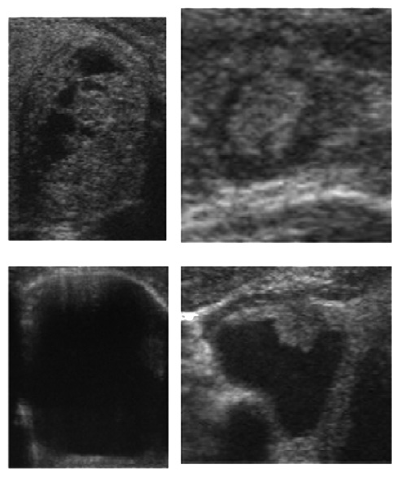
\includegraphics[width=0.40\textwidth]{2/figures/imagenes_ultrasonido_originales.png}
		\caption[Imágenes de ultrasonido de nódulos tiroideos]{Imágenes de ultrasonido de nódulos tiroideos. \\
		Fuente: \cite{pr_JERBI2023autoclassViTGAN}. \textit{Automatic classification of ultrasound thyroids images using vision transformers and generative adversarial networks}.}
		\label{2:fig210}
	\end{center}
\end{figure}


\subsection{Transfer Learning}
\cite{bk_geron2022handml} nos menciona que el Transfer Learning o Transferencia de Aprendizaje es un técnica usada en el campo de Deep Learning que permite el uso de algunas capas de un modelo ya definido y entrenado previamente en un nuevo modelo que necesite ser entrenado en una tarea similar al que se desarrolla el modelo original. Las capas destinadas al reuso son normalmente las más cercanas a la entrada o también conocidas como capas inferiores. El beneficio de usar esta técnica radica en dos puntos importantes: cantidad de datos requeridos y velocidad de entrenamiento del modelo; es decir, la cantidad de datos que se deben usar para entrenar un modelo de alto desempeño se reduce considerablemente, mientras que el tiempo requerido para terminar este proceso es menor comparándolo a si lo entrenaran desde cero.

Para que esta técnica funcione debidamente, las capas más cercanas a la salida, conocidas también como capas de alto nivel, deben ser reemplazadas, esto debido a que son más específicas de las tareas del modelo original. Esto también incluye a la capa final, ya que posiblemente no tenga la cantidad de salidas necesarias para completar satisfactoriamente la nueva tarea.

En la Figura \ref{2:fig211} se presenta de forma gráfica la técnica.

\begin{figure}[H]
	\begin{center}
		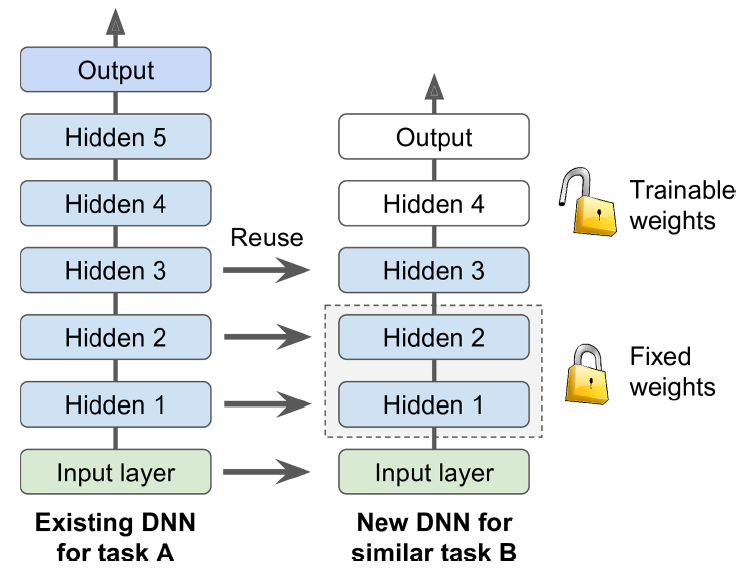
\includegraphics[width=0.70\textwidth]{2/figures/transfer_learning.PNG}
		\caption[Ejemplo de Transfer Learning]{Ejemplo de Transfer Learning. \\
		Fuente: \cite{bk_geron2022handml}. \textit{Hands-on machine learning with Scikit-Learn, Keras, and TensorFlow}.}
		\label{2:fig211}
	\end{center}
\end{figure}


\subsection{Data Augmentation}

Según \cite{bk_geron2022handml} el Aumento de Datos o Data Augmentation es una técnica de regularización que permite reforzar la cantidad de muestras en un conjunto de datos. Esto se realiza a través de la generación de nuevas instancias similares a los originales; es decir, las personas no deberían ser capaces de diferenciar una imagen generada de una del propio conjunto de datos.

Para generar estas nuevas muestras, normalmente se aplican diferentes transformaciones a las instancias del conjunto de datos original. Estas transformaciones pueden ser; por ejemplo, una simple rotación o recorte de la imagen, siempre y cuando no altere por completo su sentido como es el caso de voltear una imagen de texto de forma horizontal. 

El principal beneficio de esta técnica es que permite reducir el sobreajuste de los modelos entrenados. 

En la Figura \ref{2:fig212} se muestran algunas transformaciones que se pueden hacer al aplicar el Aumento de Datos. 

\begin{figure}[H]
	\begin{center}
		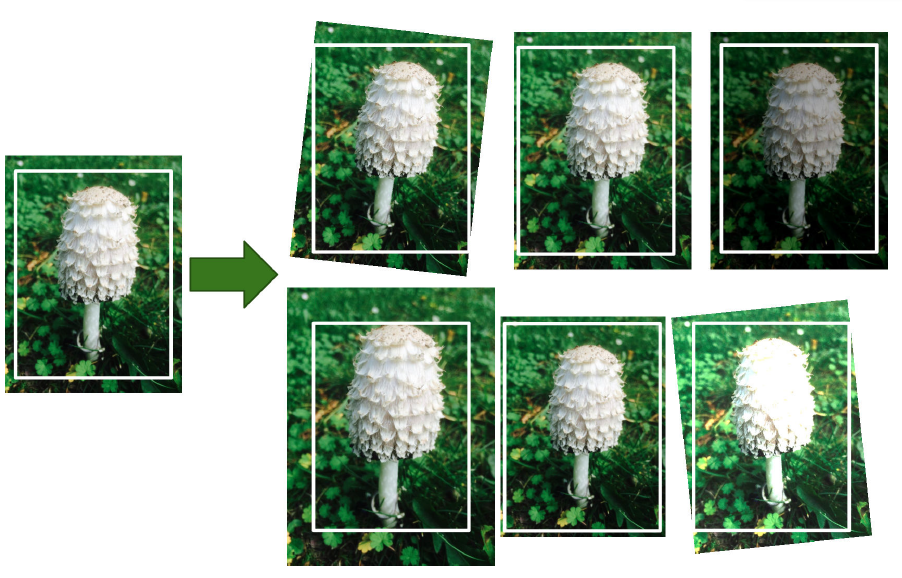
\includegraphics[width=0.85\textwidth]{2/figures/data_aug.PNG}
		\caption[Ejemplo de Data Augmentation]{Ejemplo de Data Augmentation. \\
		Fuente: \cite{bk_geron2022handml}. \textit{Hands-on machine learning with Scikit-Learn, Keras, and TensorFlow}.}
		\label{2:fig212}
	\end{center}
\end{figure}

\end{comment}

\section{Hipótesis}
\subsection{Hipótesis General}
HG: \newcommand{\HipotesisGeneral}{
El desarrollo de un Sistema de Segmentación de Características Morfológicas Faciales utilizando Redes Neuronales Convolucionales mejorará significativamente la precisión en la detección de Arrugas y Manchas}
\HipotesisGeneral


\subsection{Hipótesis Específicas}
\newcommand{\Hone}{
La utilización de un conjunto de datos diverso de imágenes faciales, que contemple características morfológicas faciales, como arrugas y manchas, incrementará la capacidad del sistema para generalizar y segmentar con precisión las características cutáneas.
}
\newcommand{\Htwo}{
Un sistema de segmentación basado en Redes Neuronales Convolucionales permitirá una detección más precisa y diferenciada de las características morfológicas faciales, tales como arrugas y manchas, superando en rendimiento a los métodos tradicionales de segmentación.
}
\newcommand{\Hthree}{
La utilización de métricas de evaluación cuantitativas, junto con una comparación sistemática entre distintas arquitecturas de Redes Neuronales Convolucionales, permitirá la identificación del modelo más eficiente en términos de precisión y rendimiento computacional en la detección de arrugas y manchas faciales.
}
\newcommand{\Hfour}{
La implementación de un sistema de segmentación de características morfológicas en tiempo real, utilizando redes neuronales convolucionales potenciadas con mecanismos de atención, permitirá el procesamiento eficaz de imágenes faciales desde video en vivo, mejorando la precisión en entornos dinámicos.
}

\begin{itemize}
	\item HE1: {\Hone}
	\item HE2: {\Htwo}
	\item HE3: {\Hthree}
	\item HE4: {\Hfour}
\end{itemize}

\chapter{Metodología de la Investigación}
\section{Diseño de la investigación}
En esta sección se detallan el diseño, tipo y enfoque de la investigación, así como la población y la muestra.

\subsection{Tipo de investigación}
Se ha identificado que este estudio posee un diseño experimental con el propósito de establecer el tipo de investigación. Como lo dice \cite{bk_hernandez2014metodologia}, en la obra titulada \citetitle{bk_hernandez2014metodologia}, busca determinar la consecuencia de una razón manipulada. Específicamente, se clasifica como un diseño experimental puro debido a la utilización intencionada de variables independientes (modificadas, eliminadas o añadidas) para evaluar su influencia en la variable dependiente, que en este caso es la segmentación avanzada de características morfológicas faciales (arrugas y manchas) en imágenes de rostros faciales.

\subsection{Enfoque de la investigación}
Este estudio adoptó un enfoque cuantitativo, conforme a lo explicado por \cite{bk_hernandez2014metodologia} en su libro \citetitle{bk_hernandez2014metodologia}. Este enfoque se basa en la recopilación de datos para comprobar hipótesis mediante mediciones numéricas y análisis estadísticos, con el objetivo de identificar patrones de comportamiento y validar teorías. La metodología empleada sigue los diez pasos del proceso cuantitativo descritos por el autor, aplicados desde la formulación de la idea hasta la presentación de los resultados finales en el informe de investigación, ya que se busca desarrollar un sistema de segmentación para detectar características morfológicas de la piel facial mediante redes neuronales convolucionales (CNN) y analizar su efectividad con métricas cuantitativas, como precisión, recall, F1-score y AUC-ROC. Este enfoque permitirá evaluar el desempeño del sistema en la detección de arrugas, poros y manchas, proporcionando resultados medibles y objetivos. \parencite{esteva2017} Al emplear técnicas de aprendizaje profundo, el estudio pretende optimizar la precisión en la segmentación de características faciales, aplicando un marco metodológico replicable y sistemático. \parencite{phillips2020}

\subsection{Población}
La población de este estudio se compone de imágenes faciales representativas de personas con diversas edades, géneros y tipos de piel. Específicamente, estas imágenes muestran características morfológicas que se asocian con arrugas y manchas faciales. Debido a la orientación del enfoque en el problemas estéticos, la población abarcaba imágenes de piel con claras imperfecciones y piel sin e incidencias asignadas. Así, el alcance de la población se determina como diverso y completo, asegurando la inclusión de imágenes que representa una amplia gama de condiciones de la piel. Finalmente, resulta esencial agregar diversidad geográfica, ya que ciertas diferencias geográficas.
\subsection{Muestra}
La muestra de la investigación comprenderá una parte de aproximadamente 5000 retratos faciales. Estas imágenes se seleccionarán mediante muestreo basado en estratos, lo que garantizará una representación uniforme en diferentes categorías de edad, identidades masculinas y femeninas y pigmentación dérmica variable La lista también tendrá imágenes con diferentes tamaños y claridad, mostrando varios tipos de arrugas y manchas, asegurándose de que el grupo muestre condiciones reales de la piel Los usaremos para enseñar, verificar y desafiar nuestro modelo de segmentación avanzada, asegurándonos de que funcione bien en la vida real con mucha variedad.

\subsection{Operacionalización de Variables}
Los detalles acerca de cómo se definen y miden las variables de estudio se presentan en la Tabla \ref{tabla:variables}.


   


%\par	%%Salto de linea
%\bigskip
\begin{flushleft}	%%Alinear a la izquierda sin justificar
	\small Fuente: Elaboración propia.
\end{flushleft}
%\end{table}

\section{Técnicas de recolección de datos}
La recolección de imágenes de características morfológicas faciales es un paso crucial para la creación del modelo de segmentación avanzada de estas. Una de las técnicas más accesibles y efectivas para obtener estas imágenes es a través del uso de bases de datos públicas como se ve en la Figura \ref{3:fig2}y repositorios en línea. Estas fuentes ofrecen una amplia variedad de imágenes de rostros faciales, que pueden ser utilizados para modelar y crear el modelo de segmentación avanzada.

\begin{figure}[h]
	\begin{center}
		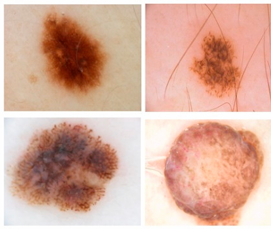
\includegraphics[width=0.75\textwidth]{3/figures/datapaper.png}
		\caption[Dataset usado en el artículo de \cite{karshiev2020improved}]{Dataset usado en el artículo de \cite{karshiev2020improved}.\\
		Fuente: \cite{karshiev2020improved}. \citetitle{karshiev2020improved}. (p. 2)}
		\label{3:fig2}
	\end{center}
\end{figure}

\begin{itemize}
    \item \textbf{Repositorios de Datasets de Imágenes Faciales}: Existen múltiples repositorios en línea dedicados específicamente a la recopilación y distribución de imágenes faciales. Plataformas como Kaggle, Papers with Code, y OpenML ofrecen conjuntos de datos etiquetados que incluyen rostros humanos con diferentes características morfológicas como arrugas, manchas, expresiones y edades. Estos datasets son fundamentales para el entrenamiento y evaluación de modelos de redes neuronales convolucionales, y suelen estar acompañados de documentación sobre su uso y licencia.
	\item \textbf{Bibliotecas Digitales y Bases de Datos Académicas}: Las bibliotecas digitales y bases de datos académicas también representan una fuente valiosa para obtener datasets faciales. En publicaciones académicas y tesis disponibles en plataformas como IEEE Xplore, SpringerLink, ScienceDirect y Google Scholar, es común encontrar referencias a datasets faciales utilizados en investigaciones previas. Estas fuentes permiten identificar conjuntos de datos validados por la comunidad científica y conocer sus aplicaciones en diferentes contextos, como el reconocimiento facial o el análisis de envejecimiento.
	\item \textbf{Plataformas de Código Abierto y Comunidades de Investigación}: Plataformas como GitHub, Hugging Face y Zenodo son ampliamente utilizadas por la comunidad investigadora para compartir datasets y modelos preentrenados. En estos repositorios, los investigadores publican conjuntos de imágenes faciales junto con scripts de preprocesamiento, anotaciones y arquitecturas de redes neuronales. Muchos de estos recursos se distribuyen bajo licencias abiertas (como CC BY o MIT).
  \end{itemize}


  %\newpage
\section{Técnicas para el procesamiento y análisis de la información}

\subsection{Metodología de implementación de la solución}

La creación de un Modelo de Segmentación Avanzada de Características Morfológicas varias fases de desarrollo, que van desde la recopilación de imágenes hasta su despliegue, como se menciona en el trabajo de \cite{yoon2023}. La imagen adquirida debe pasar por un proceso detallado posteriormente para alcanzar su etapa final. La metodología de esta investigación se muestra en la Figura \ref{3:fig3}.

\begin{figure}[h]
	\begin{center}
		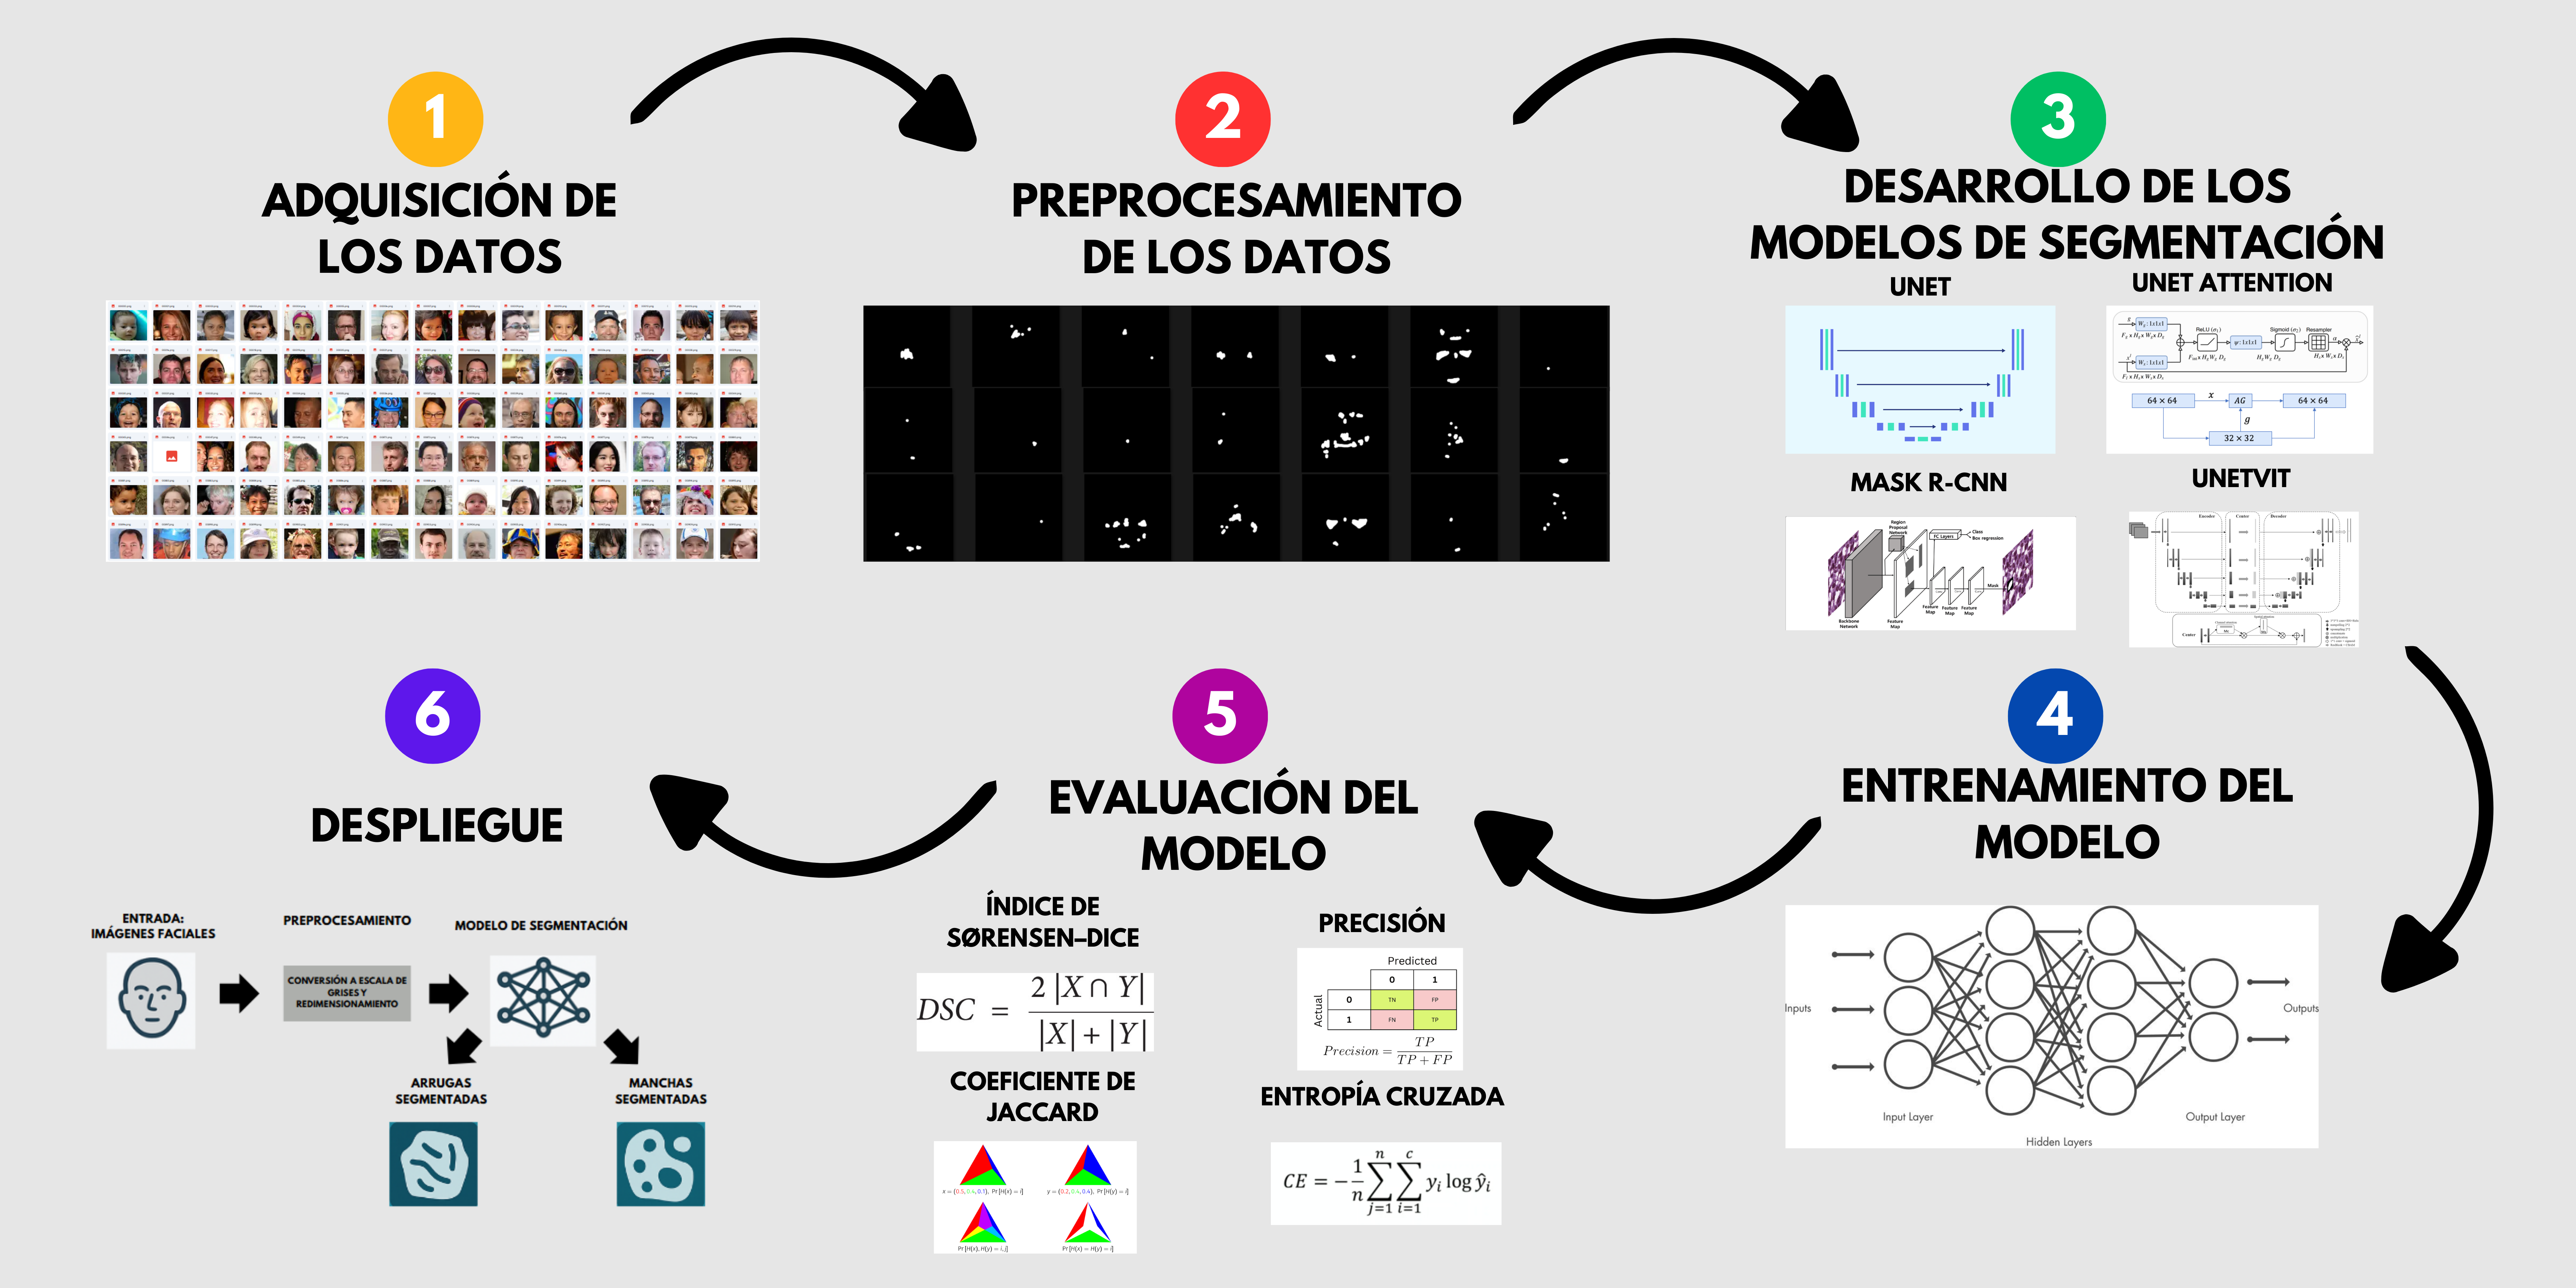
\includegraphics[width=1\textwidth]{3/figures/metodologia.png}
		\caption[Diagrama de Metodología de Investigación]{Diagrama de Metodología de Investigación.\\
			Fuente: Elaboración propia.}
		\label{3:fig3}
	\end{center}
\end{figure}


\subsubsection{Adquisición de los Datos}

En esta sección se describe el procedimiento utilizado para obtener el conjunto de datos empleado en este estudio. A continuación, se presenta una tabla que resume las tareas y actividades realizadas durante esta fase de adquisición. El primer paso fue la recopilación de datos. Los detalles sobre las actividades y tareas se encuentran en la Tabla \ref{tabla:actividades}.

Modelo ensamblado conceptualmente, listo para su implementación en entorno de desarrollo.

\subsubsection{Preprocesamiento de los Datos}
Se realizará el preprocesamiento de las imágenes del conjunto en esta etapa. La tabla \ref{tabla:preprocesamiento} incluye las tareas y actividades necesarias para completar la etapa de preprocesamiento:
\vspace{2ex}


\begin{longtable}{p{3cm}p{3cm}p{9cm}}
    \caption{Actividades de la fase de Preprocesamiento de Datos.}
    \label{tabla:preprocesamiento}\\
    \toprule
    \textbf{Actividades} & \textbf{Descripción} & \textbf{Tareas} \\
    \midrule
    \endfirsthead

    \toprule
    \textbf{Actividades} & \textbf{Descripción} & \textbf{Tareas} \\
    \midrule
    \endhead

    \bottomrule
    \endfoot

    \bottomrule
    \endlastfoot

    Filtración de imágenes faciales con características morfológicas & Eliminación de imágenes con baja resolución, mala iluminación o sin las características morfológicas de interés (arrugas y manchas), para mejorar la calidad del conjunto de datos. & 
    \begin{itemize}
        \item Eliminar imágenes borrosas, sobreexpuestas o subexpuestas.
        \item Conservar solo imágenes con resolución mínima de 128×128 píxeles.
        \item Seleccionar imágenes que contengan al menos una característica morfológica visible: arrugas o manchas.
        \item Verificar que el rostro esté completamente visible y centrado en la imagen.
    \end{itemize} \\

    Representación y normalización de las imágenes faciales & Conversión de las imágenes a formatos adecuados para su análisis por redes neuronales convolucionales. & 
    \begin{itemize}
        \item Redimensionar todas las imágenes a un tamaño uniforme.
        \item Convertir las imágenes a escala de grises o RGB, según el modelo.
        \item Normalizar los valores de píxeles entre 0 y 1.
        \item Aumentar los datos mediante técnicas como rotación, volteo, y zoom para mejorar la generalización.
    \end{itemize} \\

\end{longtable}

\begin{flushleft}
	\small Fuente: Elaboración propia.
\end{flushleft}

Enseguida, se describe en detalle las actividades junto con el resultado esperado.

\textbf{Actividad 1: Filtración de imágenes faciales con características morfológicas}
\\
En la fase de preprocesamiento de datos, la actividad de Filtración se enfoca en depurar y mejorar la calidad del conjunto de datos al eliminar información irrelevante o poco confiable. Esto se logra a través de la eliminación de datos no estándar y la conservación de aquellos que cumplen con criterios específicos de relevancia y fiabilidad. 

\textbf{Entregable}: Conjunto de datos filtrado y optimizado para su posterior análisis.

\textbf{Actividad 2: Representación y normalización de las imágenes faciales}
\\
Por otro lado, la actividad de Representación se encarga de convertir los datos en un formato visual o estructurado más adecuado para su análisis y comprensión. Esto implica transformar los datos en imágenes o representaciones gráficas que faciliten su visualización y entendimiento, contribuyendo así a una mejor interpretación por parte de los usuarios finales, como podemos observar en la Figura \ref{3:fig4}.

\textbf{Entregable}: Representación visual y estructurada de cada rostro facial en un formato adecuado para su procesamiento y análisis posterior.

\begin{figure}[h]
     \begin{center}
         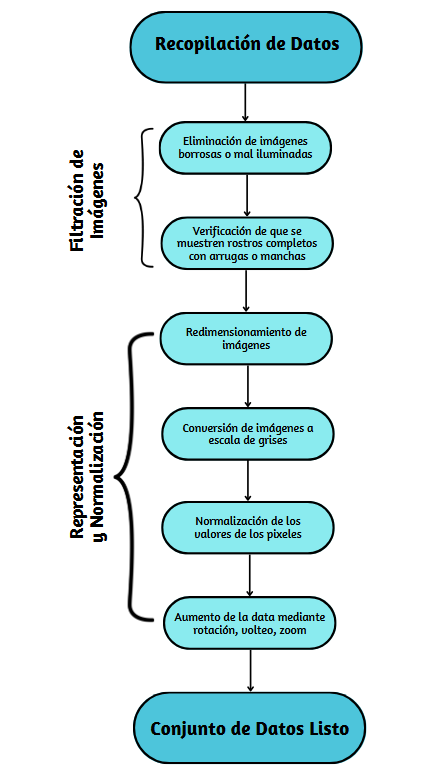
\includegraphics[width=0.75\textwidth]{3/figures/Diagrama de preprocesamiento.png}
         \caption[Diagrama de Preprocesamiento de los Datos]{Diagrama de Preprocesamiento de los Datos.\\
         Fuente: Elaboración propia}
         \label{3:fig4}
     \end{center}
 \end{figure}


 \subsubsection{Desarrollo de los Modelos de Segmentación}
 El desarrollo de los modelos de segmentación de características faciales se estructura en tres actividades clave. Estas actividades incluyen el diseño, implementación y entrenamiento de modelos basados en arquitecturas de redes neuronales profundas como U-Net, ResNet y modelos híbridos con Vision Transformer (ViT). La Tabla \ref{tabla:actividades_segmentacion} presenta el detalle de cada una.

 \vspace{2ex}
 \begingroup
 \renewcommand\arraystretch{1.2}
 \begin{longtable}{p{4cm} p{6cm} p{6cm}}
 \caption{Actividades de la fase de Desarrollo del Modelo de Segmentación.}
 \label{tabla:actividades_segmentacion}\\
 \toprule
 \textbf{Actividades} & \textbf{Descripción} & \textbf{Tareas} \\
 \midrule
 \endfirsthead
 
 \toprule
 \textbf{Actividades} & \textbf{Descripción} & \textbf{Tareas} \\
 \midrule
 \endhead
 
 \bottomrule
 \endfoot
 
 Diseño de la arquitectura del modelo & Selección conceptual y estructural de modelos apropiados para la segmentación de características morfológicas faciales. &
 \begin{itemize}
     \item Análisis de U-Net para segmentación precisa de áreas pequeñas como arrugas y poros.
     \item Evaluación del potencial de ResNet para representar características profundas y complejas.
     \item Consideración de arquitecturas híbridas que integren CNN con Vision Transformer (ViT).
 \end{itemize} \\
 
 Definición de componentes del modelo & Establecimiento de las partes esenciales del modelo para la segmentación de imágenes faciales. &
 \begin{itemize}
     \item Diseño de capas convolucionales, de codificación y decodificación.
     \item Propuesta de bloques residuales y mecanismos de atención en modelos híbridos.
     \item Configuración de dimensiones de entrada y salida adaptadas a imágenes faciales.
 \end{itemize} \\
 
 Estrategia de ensamblado del modelo & Organización lógica y estructural de los bloques que conforman cada arquitectura seleccionada. &
 \begin{itemize}
     \item Integración de módulos especializados según la arquitectura (por ejemplo, skip connections en U-Net).
     \item Planificación de rutas de información para mejorar la segmentación espacial.
     \item Definición de la estructura jerárquica de procesamiento de la imagen.
 \end{itemize} \\
 
 \end{longtable}
 \endgroup

 Enseguida, se proporciona en la Figura \ref{3:fig5} el diagrama de cada actividad, y a su vez un detalle de la actividad junto con el entregable correspondiente que se espera obtener.
 
 \textbf{Actividad 1: Diseño de la arquitectura del modelo}
 \\
 Durante esta etapa se define la estructura general de las redes neuronales que se utilizarán para la segmentación de características morfológicas faciales. El objetivo es seleccionar arquitecturas que sean adecuadas para extraer información precisa de regiones faciales como arrugas, poros o manchas.
 Entre las arquitecturas consideradas se encuentra U-Net, que destaca por su capacidad de segmentación precisa gracias a su estructura simétrica y sus conexiones de salto entre el codificador y el decodificador. También se evalúa el uso de ResNet, una arquitectura que incorpora bloques residuales para mejorar el aprendizaje en redes profundas, especialmente útil para capturar texturas complejas. Asimismo, se contempla la exploración de modelos híbridos que combinan Redes Neuronales Convolucionales (CNN) con Vision Transformer (ViT), lo cual permite captar patrones sutiles mediante mecanismos de atención.
 
 \textbf{Entregable}: Selección de la arquitectura óptima para el modelo de segmentación facial, justificada técnicamente.

 \textbf{Actividad 2: Definición de componentes del modelo}
 \\
Esta actividad consiste en establecer los elementos esenciales que conformarán las redes previamente seleccionadas. Se determina la cantidad de capas, el tipo de operaciones dentro de cada módulo y la forma en que se conectan entre sí, en función de las necesidades de segmentación facial.

En U-Net, por ejemplo, se define cuántas capas de codificación y decodificación se utilizarán, así como las conexiones que transmitirán información detallada entre estas. En ResNet, se especifica el número de bloques residuales y la profundidad de la red, asegurando que se mantenga la eficiencia del aprendizaje sin perder información relevante. En los modelos híbridos con ViT, se determina cómo integrar los módulos de atención con las capas convolucionales, de forma que se mantenga un flujo eficiente de características entre ambos entornos.

 \textbf{Entregable}: Especificación detallada de los componentes y estructura interna de cada arquitectura seleccionada.


 \textbf{Actividad 3: Estrategia de ensamblado del modelo}
 \\
 La última actividad del desarrollo se enfoca en ensamblar los componentes definidos en una arquitectura operativa y coherente. El ensamblado implica organizar los módulos en un orden lógico que permita un flujo fluido de datos desde la entrada hasta la salida del modelo.

Para U-Net, esto implica establecer correctamente las conexiones tipo “skip” que permiten recuperar detalles espaciales perdidos durante la codificación. En el caso de ResNet, se ensamblan los bloques residuales de forma que la información pueda circular libremente entre capas profundas. Finalmente, para los modelos híbridos, se debe asegurar que las características extraídas por las CNN puedan ser procesadas adecuadamente por los módulos de atención del Vision Transformer, logrando así una representación enriquecida para la segmentación facial.

 \textbf{Entregable}: Modelo ensamblado conceptualmente, listo para su implementación en entorno de desarrollo.

 
 \begin{figure}[h]
    \begin{center}
        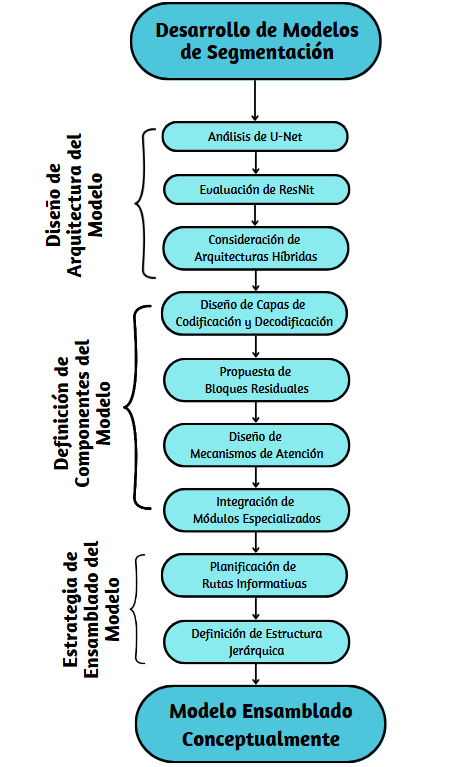
\includegraphics[width=0.75\textwidth]{3/figures/Diagrama de Desarrollo.png}
        \caption[Diagrama del Desarrollo de los Modelos de Segmentación]{Diagrama del Desarrollo de los Modelos de Segmentación.\\
        Fuente: Elaboración propia}
        \label{3:fig5}
    \end{center}
\end{figure}

\subsubsection{Entrenamiento del Modelo}
Al concluir la etapa de Desarrollo de Modelos de Segmentación, se continua con el Entrenamiento, en la Tabla \ref{tabla:entrenamiento_modelo} fue diseñada siguiendo las actividades.

\vspace{2ex}
 \begingroup
 \renewcommand\arraystretch{1.2}
 \begin{longtable}{p{4cm} p{6cm} p{6cm}}
 \caption{Actividades de la fase de Entrenamiento del Modelo.}
 \label{tabla:entrenamiento_modelo}\\
 \toprule
 \textbf{Actividades} & \textbf{Descripción} & \textbf{Tareas} \\
 \midrule
 \endfirsthead
 
 \toprule
 \textbf{Actividades} & \textbf{Descripción} & \textbf{Tareas} \\
 \midrule
 \endhead
 
 \bottomrule
 \endfoot
 
 Configuración del entorno de entrenamiento &
 Preparación del entorno computacional y los recursos necesarios para el entrenamiento del modelo. &
 \begin{itemize}
     \item Selección del framework PyTorch.
     \item Habilitación del uso de GPU para acelerar el entrenamiento.
     \item Establecimiento de rutas de acceso a los datos y modelos.
 \end{itemize} \\
 
 Aplicación de técnicas de optimización &
 Utilización de métodos que permitan una mejora progresiva del modelo a lo largo de las épocas de entrenamiento. &
 \begin{itemize}
     \item Configuración del optimizador Adam para minimizar la función de pérdida.
     \item Ajuste de tasa de aprendizaje, tamaño de batch y número de épocas.
     \item Monitorización de la evolución del loss y métricas de precisión.
 \end{itemize} \\
 
 Validación cruzada del rendimiento &
 Evaluación del desempeño del modelo utilizando múltiples divisiones del conjunto de datos. &
 \begin{itemize}
     \item División del dataset en k pliegues para pruebas y entrenamiento.
     \item Entrenamiento del modelo en diferentes subconjuntos.
     \item Análisis del promedio de métricas obtenidas para garantizar estabilidad.
 \end{itemize} \\
 
 \end{longtable}
 \endgroup

 Enseguida, se proporciona un detalle de la actividad junto con el entregable correspondiente que se espera obtener.
 
 \textbf{Actividad 1: Configuración del entorno de entrenamiento}
 \\
 Durante esta etapa se prepara el entorno computacional necesario para llevar a cabo el entrenamiento del modelo de segmentación facial. Esto implica elegir el framework de desarrollo adecuado, como PyTorch, que permite implementar arquitecturas de redes neuronales de manera eficiente. Además, se habilita el uso de aceleradores de hardware, como GPU, que reducen considerablemente el tiempo de entrenamiento. También se configuran las rutas para el acceso a los datos de entrada y se definen los parámetros básicos que utilizará el entorno de ejecución.

 \textbf{Entregable}: Entorno de entrenamiento configurado y funcional, listo para ejecutar los modelos definidos.

 \textbf{Actividad 2: Aplicación de técnicas de optimización}
 \\
 En esta fase se aplican técnicas diseñadas para mejorar el aprendizaje del modelo durante el entrenamiento. Se implementa el optimizador Adam, ampliamente utilizado por su capacidad de ajustar dinámicamente los parámetros de la red, favoreciendo una convergencia más rápida y estable. Se determinan parámetros críticos como la tasa de aprendizaje, el tamaño del lote (batch size) y el número total de épocas, adaptándolos al comportamiento del modelo y la complejidad del conjunto de datos. Además, se monitorean continuamente la función de pérdida (loss) y las métricas de precisión para evaluar el progreso del modelo.

 \textbf{Entregable}: Modelo entrenado con parámetros de optimización ajustados, y registro de métricas de desempeño durante las épocas.

 \textbf{Actividad 3: Validación cruzada del rendimiento}
 \\
 El objetivo de esta actividad es evaluar de manera robusta el rendimiento del modelo mediante la técnica de validación cruzada. Se divide el conjunto de datos en k pliegues, permitiendo entrenar y validar el modelo en diferentes combinaciones de subconjuntos. Esta estrategia ayuda a prevenir el sobreajuste (overfitting) y asegura que el desempeño del modelo no dependa exclusivamente de una sola partición del dataset. Finalmente, se analiza el promedio de métricas obtenidas en cada iteración para validar la estabilidad y generalización del modelo.

 \textbf{Entregable}: Reporte de resultados de validación cruzada con métricas promedio y análisis de estabilidad del modelo.

\subsubsection{Evaluación del Modelo}
En esta etapa, se lleva a cabo la evaluacion de los prototipos elaborados en este trabajo, en la seccion 3.3.2 se está empleando las métricas de clasificación seleccionadas y detalladas. Se ofrece un analisis pormenorizado de las actividades y tareas ejecutadas en esta fase en la Tabla \ref{tabla:evaluacion_modelo}.

\vspace{2ex}
 \begingroup
 \renewcommand\arraystretch{1.2}
 \begin{longtable}{p{4cm} p{6cm} p{6cm}}
 \caption{Actividades de la fase de Evaluación del Modelo.}
 \label{tabla:evaluacion_modelo}\\
 \toprule
 \textbf{Actividades} & \textbf{Descripción} & \textbf{Tareas} \\
 \midrule
 \endfirsthead
 
 \toprule
 \textbf{Actividades} & \textbf{Descripción} & \textbf{Tareas} \\
 \midrule
 \endhead
 
 \bottomrule
 \endfoot
 
 Preparación de Datos de Validación & Seleccionar y preparar un conjunto de datos de validación representativo. & 
 \begin{itemize}
     \item Elección de imágenes que no hayan sido empleados en el proceso de entrenamiento.
     \item Preprocesamiento de imágenes.
 \end{itemize} \\
 
 Definición de Métricas de Evaluación & Definir métricas cuantitativas para evaluar al modelo de segmentación. & 
 \begin{itemize}
     \item Identificación de métricas adecuadas.
     \item Implementación de funciones para calcular estas métricas.
 \end{itemize} \\
 
 Evaluación del Modelo & Evaluar el modelo entrenado en el conjunto de datos de validación para obtener una línea base. & 
 \begin{itemize}
     \item Eficiencia del modelo de segmentación en el conjunto de validación.
     \item Cálculo de métricas de evaluación.
 \end{itemize} \\
 
 \end{longtable}
 \endgroup

 \textbf{Actividad 1: Preparación de Datos de Validación}
 \\
 La preparación de los datos de validación desempeña un papel crucial en la evaluación de la efectividad del modelo en datos no previamente vistos. Esta tarea implica seleccionar un subconjunto representativo del conjunto de datos que no se haya utilizado durante el entrenamiento del modelo. La selección debe tener en cuenta la diversidad en las imágenes y sus configuraciones para garantizar que el modelo pueda generalizar correctamente a diferentes escenarios.
 
 \textbf{Entregable}: Un conjunto de datos listo para su uso en la evaluación del modelo, que incluye imágenes preprocesadas y listas para ser utilizadas en el análisis.
 
 \textbf{Actividad 2: Definición de Métricas de Evaluación}
 \\
 Para evaluar el rendimiento del modelo de manera cuantitativa, es esencial definir métricas claras. Estas métricas proporcionarán una base objetiva para comparar el rendimiento del modelo en diferentes escenarios y con otros enfoques existentes.
 
 \textbf{Entregable}: Un documento detallado que describe cada métrica y proporciona el código o las funciones necesarias para calcularlas.
 
 \textbf{Actividad 3: Evaluación del Modelo}
 \\
 La evaluación del modelo involucra el uso del conjunto de datos de validación para establecer un punto de referencia sobre su rendimiento. Esta evaluación es esencial para comprender el comportamiento del modelo en situaciones no previamente vistas durante el entrenamiento y para identificar posibles áreas de mejora.
 
 \textbf{Entregable}: Un informe que presenta los resultados de la evaluación inicial, incluyendo las métricas de rendimiento calculadas y cualquier observación relevante sobre el comportamiento del modelo.
 
\subsubsection{Despliegue}
Al concluir la metodología empleada, se procedió a implementar el modelo propuesto luego de finalizar su entrenamiento y evaluación correspondiente. Los pasos y tareas realizados en esta fase se encuentran detallados en la Tabla \ref{tabla:despliegue}.

\vspace{2ex}
 \begingroup
 \renewcommand\arraystretch{1.2}
 \begin{longtable}{p{4cm} p{6cm} p{6cm}}
 \caption{Actividades de la fase de Despliegue.}
 \label{tabla:despliegue}\\
 \toprule
 \textbf{Actividades} & \textbf{Descripción} & \textbf{Tareas} \\
 \midrule
 \endfirsthead
 
 \toprule
 \textbf{Actividades} & \textbf{Descripción} & \textbf{Tareas} \\
 \midrule
 \endhead
 
 \bottomrule
 \endfoot
 
 Preparación del Entorno de Despliegue & Configurar el entorno necesario para desplegar el modelo en producción. & 
    \begin{itemize}
        \item Selección de infraestructura.
        \item Configuración del entorno de hardware y software.
        \item Pruebas iniciales.
    \end{itemize} \\
 
 Despliegue del Modelo en Producción & Implementar el modelo en el entorno de producción para su uso real. & 
 \begin{itemize}
     \item Implementación del modelo en producción.
     \item Configuración de parámetros en tiempo de ejecución.
     \item Monitoreo inicial del desempeño.
 \end{itemize} \\
 \end{longtable}
 \endgroup

\textbf{Actividad 1: Preparación del Entorno de Despliegue}
\\
La preparación del entorno de despliegue es una etapa fundamental para asegurar que el modelo de segmentación pueda ser ejecutado eficientemente en producción. Este proceso implica la selección y configuración de la infraestructura necesaria, incluyendo tanto hardware como software, y la realización de pruebas iniciales para confirmar que todo funciona correctamente antes del despliegue completo.

\textbf{Entregable}: Un entorno completamente preparado, con todos los componentes necesarios instalados y configurados, listo para el despliegue del modelo.

\textbf{Actividad 2: Despliegue del Modelo en Producción}
\\
El despliegue del modelo en producción es el paso en el que el modelo de segmentación se pone en funcionamiento en el entorno de producción. Este proceso incluye la implementación del modelo, la configuración de parámetros necesarios para su ejecución en tiempo real, y el monitoreo inicial para asegurar que el modelo funciona correctamente en condiciones reales.

\textbf{Entregable}: El modelo está completamente implementado y operando en el entorno de producción, con los parámetros ajustados y el desempeño monitoreado para asegurar su correcto funcionamiento.

\section{Metodología para la Medición de Resultados de la Implementación}

Diversas métricas se emplean para evaluar el desempeño de un modelo, en los datos de la Matriz de Confusión, sirviendo como herramientas de evaluación fundamentadas. A continuación, se describe su significado y sus componentes.

\begin{itemize}
\item \textbf{Matriz de confusión}: Tabla de dimensiones que sintetiza la precisión de predicciones generadas por un protitopo de categorización. La matriz muestra la relación entre las etiquetas predichas por el modelo y las etiquetas reales de los datos. Uno de los ejes de la matriz representa las etiquetas predichas, mientras que el otro muestra las etiquetas reales, con N representando el número total de clases. Su propósito primario es analizar la eficacia de un modelo de Aprendizaje Automático Supervisado en conjuntos de datos de prueba, donde las etiquetas reales son desconocidas. El término <<matriz de confusión>> se origina porque ayuda a identificar dónde el sistema confunde entre dos clases (Big Data, 2019). en la Figura \ref{3:fig7}, se puede encontrar una representación visual de la matriz de confusión.
\begin{figure}[H]
	\centering
	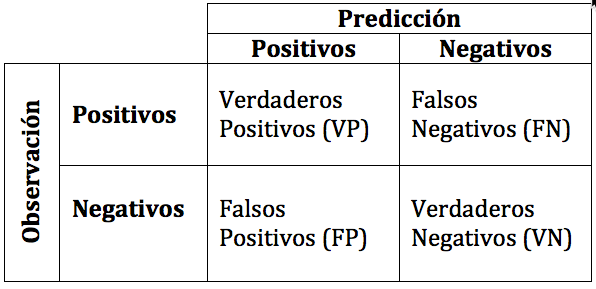
\includegraphics[width=0.75\textwidth]{3/figures/matriz_confusion.png}
	\caption[Matriz de Confusión]{Matriz de Confusión.\\ Fuente: \cite{izco2018bdc}. \citetitle{izco2018bdc}.}
	\label{3:fig7}
\end{figure}
\end{itemize}

\begin{itemize}
    \item \textbf{Verdaderos Positivos}: Se denomina verdadero positivo cuando el modelo realiza una predicción precisa de la clase positiva.
    \item \textbf{Verdaderos Negativos}: Se trata de un verdadero negativo cuando el modelo realiza una predicción correcta de la clase negativa.
    \item \textbf{Falsos Positivos}: Ocurre un falso positivo cuando el modelo hace una predicción incorrecta de la clase positiva. 
    \item \textbf{Falsos Negativos}: Ocurre un falso negativo cuando el modelo hace una predicción incorrecta de la clase negativa. 
    \end{itemize}

Después de explicar los conceptos anteriores, se obtienen diferentes métricas, de las cuales solo se utilizará la precisión métrica según lo referenciado en los documentos anteriores:

\textbf{Precisión}: evalúa la fracción de elementos detectados adecuadamente como positivos entre todos los elementos identificados como positivos. Su cálculo se basa en la siguiente expresión.
        \begin{equation}\label{eq:precision}
            \phantomsection
            \text{Precisión}=\frac{V.P.}{V.P.+F.P.}
            \end{equation}
        \myequations{Fórmula para la precisión}
        
        La pregunta que responde esta métrica es: ¿Cuál es la proporción de segmentaciones positivas que son precisas?


Además, hemos tomado otra métricas para evaluar el rendimiento del modelo de segmentación, las cuales se explicarán a continuación:

\textbf{Índice de Sørensen–Dice (Dice Similarity Coefficient - DSC)}
El índice de Sørensen-Dice es una medida estadística utilizada para evaluar la similitud entre dos muestras. En el contexto de segmentación de imágenes, cuantifica la superposición entre la segmentación predicha y la verdadera (ground truth). \parencite{taha2015metrics}
        
Se define como:
        
\begin{equation}
    \text{DSC} = \frac{2 \times |A \cap B|}{|A| + |B|}
\end{equation}
\myequations{Fórmula del Índice de Sørensen–Dice (DSC)}

\noindent Donde:
\begin{itemize}
    \item $|A|$ representa el número de píxeles predichos como positivos por el modelo.
    \item $|B|$ representa el número de píxeles verdaderamente positivos (segmentación real).
    \item $|A \cap B|$ es el número de píxeles correctamente clasificados como positivos (verdaderos positivos).
\end{itemize}

\noindent El Índice de Sørensen–Dice mide la superposición entre la predicción y la verdad real, con un rango de valores entre $0$ (sin coincidencia) y $1$ (coincidencia perfecta).
     

\textbf{Coeficiente de Jaccard (Índice de Intersección sobre Unión - IoU)}
El Coeficiente de Jaccard o IoU (Intersection over Union) mide la proporción de la intersección entre el área segmentada correctamente y la unión de todas las áreas predichas y reales. Es una de las métricas más comunes en segmentación de imágenes. \parencite{reinke2021common}
        
\begin{equation}
    \text{IoU} = \frac{|A \cap B|}{|A \cup B|}
\end{equation}
\myequations{Fórmula del Coeficiente de Jaccard (Intersection over Union)}

\noindent Donde:
\begin{itemize}
    \item $|A|$ es el conjunto de píxeles positivos predichos.
    \item $|B|$ es el conjunto de píxeles positivos reales.
    \item $|A \cap B|$ representa los píxeles clasificados correctamente como positivos (verdaderos positivos).
    \item $|A \cup B|$ representa el total de píxeles positivos predichos o reales (la unión de ambos conjuntos).
\end{itemize}

\noindent El Coeficiente de Jaccard mide la proporción de superposición respecto al total combinado de las regiones predicha y real.
                     
El Coeficiente de Jaccard tiende a ser más estricto que el índice de Dice, ya que penaliza con mayor fuerza las falsas predicciones. Se considera una métrica robusta para segmentaciones de alta precisión. \parencite{reinke2021common}

\textbf{Entropía Cruzada (Cross-Entropy Loss)}
La entropía cruzada es una función de pérdida ampliamente usada para tareas de clasificación y segmentación semántica, especialmente cuando se aplica un modelo que produce probabilidades para cada clase (como softmax o sigmoid). \parencite{goodfellow2016deep}

\begin{equation}
    \text{CE} = -\sum_{i=1}^{N} y_i \log(\hat{y}_i)
\end{equation}
\myequations{Fórmula de Entropía Cruzada (Cross-Entropy Loss)}

\noindent Donde:
\begin{itemize}
    \item $N$ es el número total de muestras (píxeles o instancias).
    \item $y_i$ es la etiqueta verdadera de la clase para la muestra $i$.
    \item $\hat{y}_i$ es la probabilidad predicha por el modelo para esa clase.
\end{itemize}

\noindent La Entropía Cruzada penaliza más fuertemente las predicciones con alta confianza que resultan incorrectas, y se minimiza durante el entrenamiento del modelo.

En segmentación binaria, esta función penaliza más las clasificaciones incorrectas cuanto más seguras son las predicciones erróneas. Se considera una métrica adecuada para entrenar redes neuronales cuando se requiere distinguir entre fondo y objeto. \parencite{goodfellow2016deep}

\begin{landscape}
	\section{Cronograma de actividades y presupuesto}
	Se propuso un cronograma para la investigación. Conforma desde el inicio hasta ser terminada con la sustentación final planeada para mediados del año 2024. Este se presneta en la Figura \ref{3:fig6}.

	\begin{figure}[!ht]
		\begin{center}
			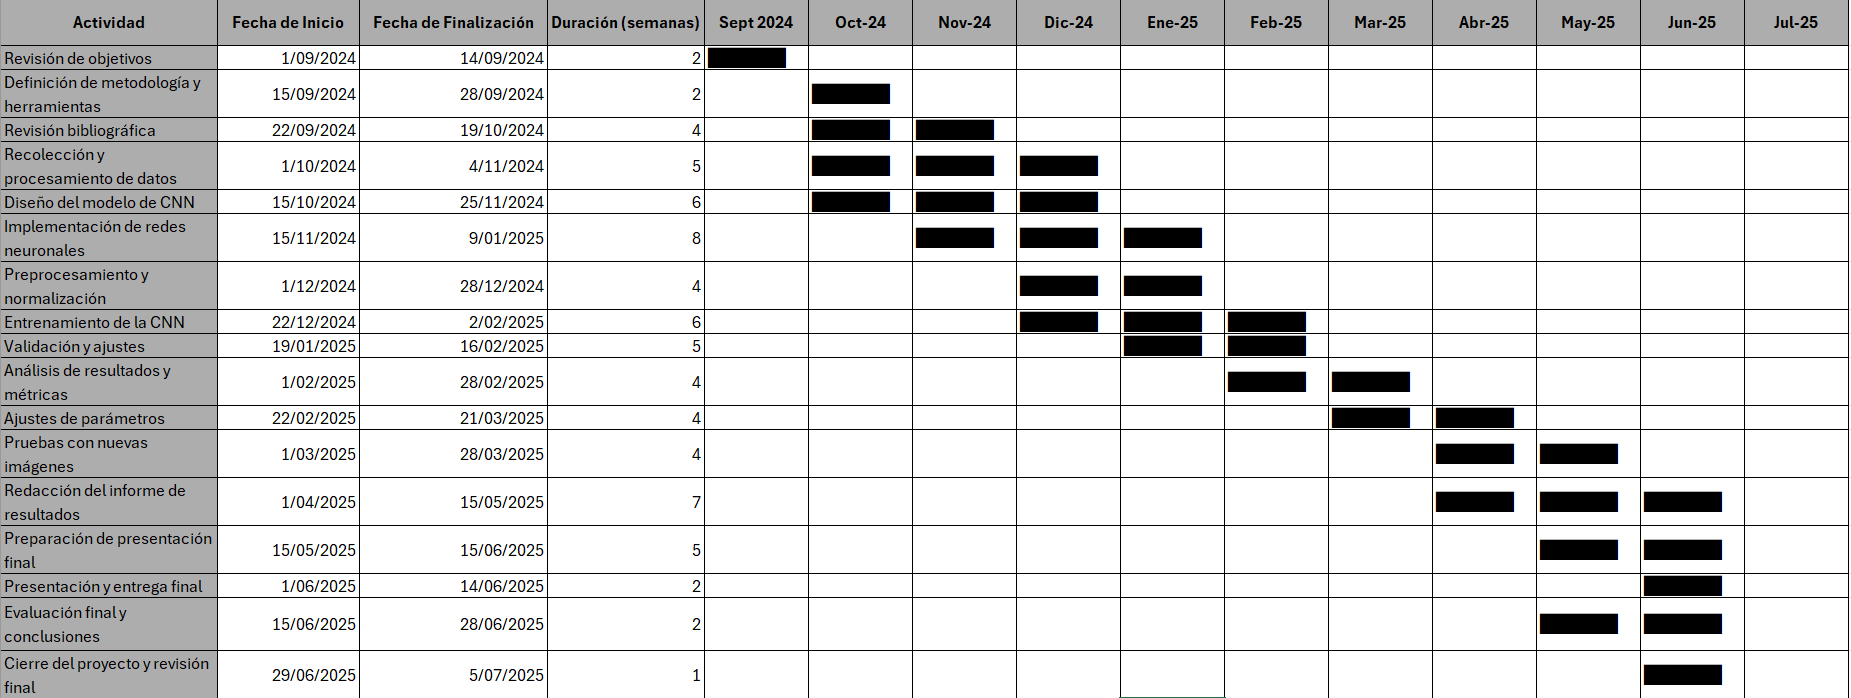
\includegraphics[width=1.50\textwidth]{3/figures/gant.png}
			\caption[Cronograma de actividades]{Cronograma de actividades.\\
				Fuente: Elaboración propia.}
			\label{3:fig6}
		\end{center}
	\end{figure}
	
\end{landscape}
%%%%%%%%%%%%%%%%%%%%%%%%%%%%%%%%%%%%%%%%

%%%%%%%%%%%%%%%%%%%%%%%%%%%%%%%



La Tabla \ref{tab:presupuesto} detalla los gastos relacionados con la investigación, incluyendo la compra de herramientas como una computadora portátil antes del inicio del proyecto, así como los costos asociados a actividades generales y al proceso de redacción y presentación pública de la tesis.

\begin{table}[h!]
	\caption{Presupuesto}
	\label{tab:presupuesto}
	\centering
	\small
	\begin{tabular}{p{6cm}rrr}
		\toprule
		\textbf{Concepto} & \textbf{Horas empleadas} & \textbf{Gasto (en soles)} & \textbf{Total} \\
		\midrule
		\multicolumn{4}{l}{\textbf{Activos físicos}} \\
		Portátil Lenovo Ideapad S340-15IIL Core i7 de 10ma GEN & -- & S/.5,700.00 & S/.5,700.00 \\
		\midrule
		\multicolumn{4}{l}{\textbf{Honorarios por el proceso de elaboración y defensa pública de la tesis}} \\
		Tasa de registro para el tema de investigación & -- & S/.800.00 & S/.800.00 \\
		Apartado del tema de tesis & -- & S/.2,700.00 & S/.2,700.00 \\
		Honorarios de defensa & -- & S/.1,500.00 & S/.1,500.00 \\
		\midrule
		\multicolumn{4}{l}{\textbf{Personal o equipo humano}} \\
		Progreso de tesis & 1000 & Inconmensurable & -- \\
		\midrule
		\multicolumn{4}{l}{\textbf{Gastos operativos}} \\
		Conexión a internet y servicio de electricidad (durante 8 meses) & 200 & S/.50.00 & S/.1000.00 \\
		\midrule
		\textbf{Python} & 50 & - & - \\
		\midrule
		\textbf{Suma total} & 1250 & -- & S/.11,700.00 \\
		\bottomrule
	\end{tabular}
	\begin{flushleft}
		\small Fuente: Elaboración propia.
	\end{flushleft}
\end{table}





\chapter{Desarrollo de la Solución}
Dentro de esta sección se expone con precisión el procedimiento descrito previamente en la sección anterior, correspondiente a cada acción incluida en la metodología implementada, junto con los entregables previstos.

\section{Adquisición de los Datos}

\textbf{Actividad 1: Identificación de la data que contengan imágenes de rostros con características morfológicas faciales de proporciones similares}
 
Con el objetivo de entrenar un modelo de segmentación enfocado en características morfológicas faciales como arrugas y manchas, se llevó a cabo una exhaustiva búsqueda de bases de datos públicas en repositorios especializados. Se priorizó la recolección de conjuntos de datos que incluyeran imágenes faciales en alta resolución, variedad de edades, géneros y tonos de piel, así como condiciones de iluminación lo suficientemente controladas como para facilitar la segmentación de detalles faciales sutiles.

Durante este proceso, se identificaron diversos repositorios en plataformas como GitHub que ofrecían acceso a bases de datos con más de 200,000 imágenes faciales. Entre los conjuntos más destacados se encuentran versiones extendidas de datasets como CelebA, FFHQ (Flickr-Faces-HQ), y otros compendios curados por la comunidad investigadora, que contienen imágenes faciales etiquetadas o anotadas para tareas de reconocimiento y análisis facial.

Sin embargo, debido al enfoque específico de esta investigación la segmentación de características morfológicas finas como arrugas y manchas fue necesario realizar una selección cuidadosa de las imágenes más adecuadas. Para ello, se aplicaron criterios de claridad visual, resolución suficiente y visibilidad explícita de las deformaciones morfológicas faciales. Como resultado de este filtrado, se seleccionó un subconjunto compuesto por 5,000 imágenes faciales que cumplían con los siguientes criterios:

\begin{itemize}
    \item Alta calidad visual.   
    \item Visibilidad clara de texturas de la piel.
    \item Presencia evidente de arrugas y manchas.
    \item Proporciones faciales dentro de un rango estándar para facilitar el modelado.
\end{itemize} 

Este conjunto reducido pero representativo,lo podemos ver en la Figura \ref{4:fig1}, constituye la base de entrenamiento y validación del modelo propuesto. La selección manual de estos datos buscó optimizar el desempeño del modelo, al exponerlo exclusivamente a ejemplos que contienen información útil para aprender patrones asociados a las características morfológicas de interés.

\begin{figure}[h]
	\begin{center}
		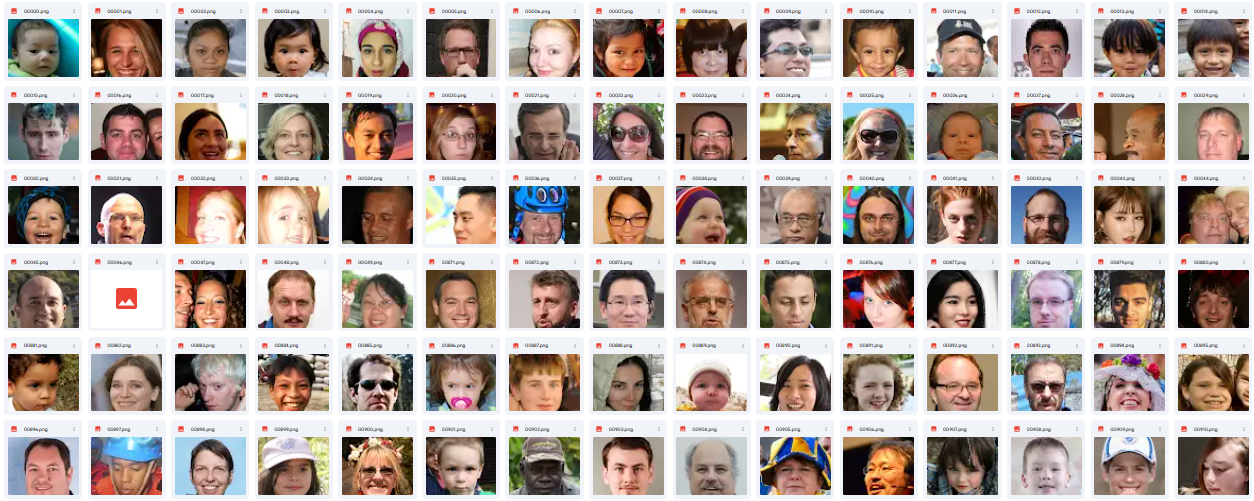
\includegraphics[width=0.75\textwidth]{4/figures/data.png}
		\caption[Dataset recolectado de repositorios]{Dataset recolectado de repositorios.\\
		Fuente: Elaboración propia}
		\label{4:fig1}
	\end{center}
\end{figure}

\section{Preprocesamiento de los Datos}

\textbf{Actividad 1: Filtración de imágenes faciales con características morfológicas}

Una vez recopilado el subconjunto de 5,000 imágenes faciales con características morfológicas visibles, se procedió a una etapa de filtración adicional orientada a reforzar la consistencia y la relevancia de los datos para la tarea de segmentación. Esta filtración se enfocó en garantizar que todas las imágenes seleccionadas contuvieran arrugas y manchas claramente identificables, descartando aquellas que, pese a su calidad visual, no presentaban estas características de manera explícita.

El proceso se realizó mediante una inspección semiautomática, apoyada en técnicas básicas de detección de texturas y realce de bordes para facilitar la identificación visual de las zonas con deformaciones. Como resultado, se aseguraron condiciones homogéneas entre las imágenes del dataset final, lo que permitió una base sólida para la generación de máscaras de segmentación precisas.

\textbf{Actividad 2: Representación y normalización de las imágenes faciales}

Con el conjunto de imágenes definitivo, se ejecutó un proceso de preprocesamiento estandarizado con dos objetivos principales: uniformar las dimensiones espaciales de las imágenes y generar las máscaras binarias asociadas a las regiones con deformaciones morfológicas.

En primer lugar, todas las imágenes fueron redimensionadas a una resolución uniforme de 1024x1024 píxeles, preservando la relación de aspecto y aplicando interpolación bilineal para mantener la calidad visual. Esta estandarización es fundamental para asegurar la compatibilidad estructural con las redes neuronales convolucionales utilizadas en etapas posteriores, y facilita la aplicación de operaciones convolucionales sobre áreas homogéneas.

En segundo lugar, se generaron máscaras binarias (en blanco y negro) correspondientes a cada imagen. Estas máscaras representan las regiones específicas del rostro que contienen arrugas, manchas u otras alteraciones morfológicas, codificadas de la siguiente manera:

\begin{itemize}
    \item Blanco (valor 1): Regiones con características morfológicas relevantes (objetivo de segmentación).   
    \item Negro (valor 0): Regiones sin interés morfológico.
\end{itemize} 

Las máscaras, como se ve en la Figura \ref{4:fig2}, fueron elaboradas a partir de una combinación de anotación semiautomática y herramientas de realce de texturas, contrastes y gradientes, con verificación manual en una muestra aleatoria para asegurar su validez.

\begin{figure}[h]
	\begin{center}
		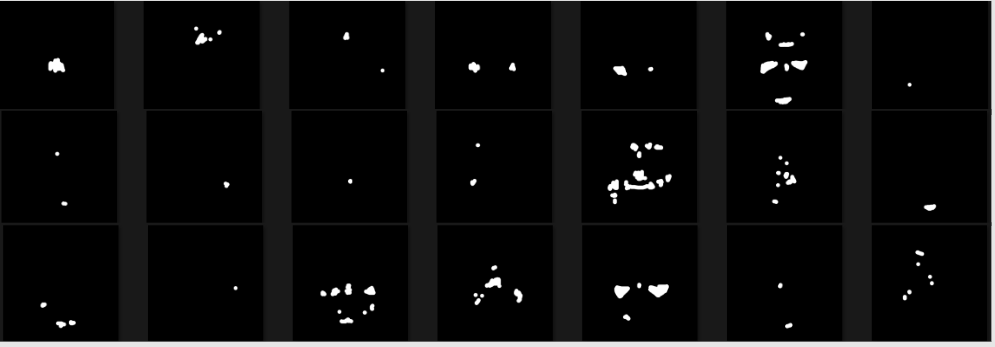
\includegraphics[width=0.75\textwidth]{4/figures/mascaras.png}
		\caption[Máscaras binarias generadas]{Máscaras binarias generadas.\\
		Fuente: Elaboración propia}
		\label{4:fig2}
	\end{center}
\end{figure}

Este proceso de representación y normalización, como se ve en el diagrama final de Preprocesamiento en la Figura \ref{4:fig3}, permitió convertir los datos originales en pares de entrada (imagen facial) y salida (máscara de segmentación), aptos para el entrenamiento supervisado del modelo de segmentación basado en redes neuronales convolucionales.

\begin{figure}[h]
	\begin{center}
		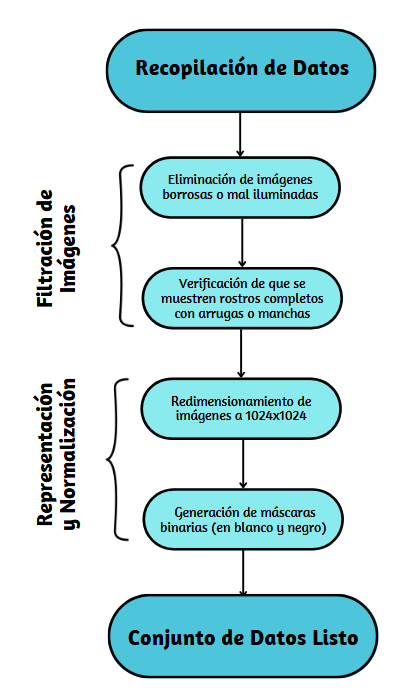
\includegraphics[width=0.45\textwidth]{4/figures/diagrama final prepo.png}
		\caption[Diagrama de Preprocesamiento Utilizado]{Diagrama de Preprocesamiento Utilizado.\\
		Fuente: Elaboración propia}
		\label{4:fig2}
	\end{center}
\end{figure}

\section{Desarrollo de los Modelos de Segmentación}

\textbf{Actividad 1: Diseño de la arquitectura del modelo}\\
Se diseñó una arquitectura basada en U-Net con Attention Gates, que consta de:
\begin{itemize}
  \item Módulos de doble convolución (DoubleConv) en el encoder y decoder.  
  \item Capas de atención (AttentionGate) ubicadas en cada salto del decoder para realzar las regiones de interés (arrugas y manchas).  
  \item Caminos de downsampling (MaxPool2d) y upsampling (ConvTranspose2d) para conservar la resolución espacial.  
  \item Capa final de convolución 1x1 para segmentación en tres clases (fondo, arrugas, manchas).  
\end{itemize}

\textbf{Actividad 2: Definición de componentes del modelo}\\
Los componentes principales incluyen:
\begin{itemize}
  \item \textit{DoubleConv}: bloque de dos convoluciones secuenciales con BatchNorm y ReLU.  
  \item \textit{AttentionGate}: mecanismo de atención consistente en convoluciones 1x1, sumas tensoriales y función Sigmoid para generar máscaras atencionales.  
  \item Optimizador \texttt{AdamW} con decaimiento de pesos para mejorar la generalización.  
  \item Scheduler \texttt{ReduceLROnPlateau} para ajuste dinámico de la tasa de aprendizaje.  
  \item Función de pérdida \texttt{CrossEntropyLoss} con pesos calculados por median frequency balancing.  
\end{itemize}

\textbf{Actividad 3: Estrategia de ensamblado del modelo}\\
Se definió una estrategia de ensamblado simple basada en el entrenamiento de un solo modelo entrenado por 50 épocas, guardando el estado de mejor rendimiento en validación (menor pérdida). No se implementó ensamblado múltiple, pues la arquitectura con atención demostró ser suficiente tras el análisis de métricas.

\section{Entrenamiento del Modelo}

\textbf{Actividad 1: Configuración del entorno de entrenamiento}\\
Se configuró el entorno con los siguientes parámetros:
\begin{itemize}
  \item Ruta de datos: \texttt{face\_images}, \texttt{arrugas}, \texttt{manchas}.  
  \item Tamaño de lote (batch size): 4.  
  \item Dimensión de entrada: 256 x 256 píxeles.  
  \item Tasa de aprendizaje inicial: $1\times10^{-4}$.  
  \item Número de épocas: 50.  
  \item Dispositivo de cómputo: GPU (CUDA) o CPU según disponibilidad.  
  \item Semilla aleatoria fija (42) para reproducibilidad.  
\end{itemize}

\textbf{Actividad 2: Aplicación de técnicas de optimización}\\
Se incorporaron las siguientes técnicas:
\begin{itemize}
  \item Aumentos de datos con \texttt{albumentations}: volteos, rotaciones, ruido Gaussiano, brillo/contraste, transformaciones elásticas y desenfoque.  
  \item Balanceo de clases mediante median frequency balancing para generar pesos en \texttt{CrossEntropyLoss}.  
  \item Optimizador \texttt{AdamW} y scheduler \texttt{ReduceLROnPlateau} para ajuste automático de la tasa de aprendizaje.  
  \item Impresión de métricas de pérdida en entrenamiento y validación por época.  
\end{itemize}

\textbf{Actividad 3: Validación cruzada del rendimiento}\\
La validación se realizó con:
\begin{itemize}
  \item División de datos: 80\% entrenamiento, 20\% validación usando \texttt{train\_test\_split}.  
  \item DataLoaders separados para entrenamiento y validación, garantizando evaluación independiente.  
  \item Cálculo de métricas (pérdida, precisión, Dice, Jaccard) en el conjunto de validación cada época.  
  \item Guardado del modelo con menor \emph{val\_loss} como mejor checkpoint.  
\end{itemize}


\section{Evaluación del Modelo}

\textbf{Actividad 1: Preparación de Datos de Validación}\\
Se prepararon las imágenes de validación con transformaciones mínimas:
\begin{itemize}
  \item Redimensionamiento a 256x256 píxeles.  
  \item Conversión a tensor SIN alteraciones adicionales.  
  \item Unión de máscaras de arrugas y manchas en una única máscara multicategoría.  
\end{itemize}

\textbf{Actividad 2: Definición de Métricas de Evaluación}\\
Las métricas utilizadas fueron:
\begin{itemize}
  \item \textit{Precision} (macro) para evaluar la exactitud de las predicciones.  
  \item \textit{Dice Score} promedio para medir la superposición.  
  \item \textit{Jaccard Index (IoU)} promedio para una evaluación estricta del solapamiento.  
\end{itemize}

\textbf{Actividad 3: Evaluación del Modelo}\\
El modelo alcanzó los siguientes resultados en validación:
\begin{itemize}
  \item \textbf{Pérdida mínima (val\_loss):} 0.0458 (época 50).  
  \item \textbf{Precision promedio:} 0.645.  
  \item \textbf{Dice Score promedio:} 0.440.  
  \item \textbf{Jaccard Index promedio:} 0.289.  
  \item Se observaron mejores resultados en la detección de arrugas debido a mayor representación de esta clase.  
  \item La clase ":manchas" mostró métricas ligeramente inferiores, sugiriendo futuras mejoras en aumentos específicos.  
\end{itemize}

Los resultados numéricos y ejemplos de segmentaciones se presentan en la sección de análisis de resultados con gráficas de evolución y comparaciones visuales.


\section{Despliegue}

\textbf{Actividad 1: Preparación del Entorno de Despliegue}

\textbf{Actividad 2: Despliegue del Modelo en Producción}

\chapter{Conclusiones y Recomendaciones}
\section{Conclusiones}
Una vez definido el problema central relacionado con la segmentación automatizada de deformaciones morfológicas faciales y establecido el marco de objetivos e hipótesis, se logró cumplir con el propósito general de esta investigación: diseñar un sistema capaz de segmentar arrugas y manchas en imágenes faciales mediante Redes Neuronales Convolucionales. Este objetivo se abordó considerando como criterio principal el uso exclusivo de imágenes faciales humanas y, como enfoque metodológico, la implementación de un modelo de aprendizaje profundo basado en redes neuronales convolucionales, específicamente una arquitectura U-Net con mecanismos de atención.

En relación con los objetivos específicos, se evidenció que el análisis de modelos propuestos en investigaciones previas tuvo un impacto significativo en la selección de características relevantes y en la construcción del enfoque metodológico adoptado. Esta revisión permitió validar hipótesis provenientes de la literatura sobre el desempeño superior de arquitecturas basadas en redes neuronales convolucionales frente a enfoques tradicionales de aprendizaje automático, especialmente en tareas de segmentación de imágenes. Los resultados obtenidos, como se ven el Tabla \ref{tab:result_models}, durante las fases de evaluación cuantitativa respaldan esta elección, demostrando mejoras sustanciales en métricas como loss, precisión, Dice Score e IoU.

A partir de los resultados mostrados en la Tabla \ref{tab:result_models}, se concluye que el modelo U-Net con mecanismos de atención obtuvo el mejor desempeño global en la tarea de segmentación de características morfológicas faciales, superando significativamente a sus variantes y a otras arquitecturas evaluadas. Este modelo logró una pérdida (entropía cruzada) de 0.1158 y una precisión de 0.911, posicionándose por encima del U-Net estándar y de U-Net con codificador MiT-B0, así como muy por delante de Mask R-CNN, que mostró un rendimiento considerablemente inferior. Las métricas del índice de Sørensen–Dice (0.810) y el coeficiente de Jaccard (0.852) reflejan la eficacia del modelo propuesto en términos de solapamiento con las segmentaciones reales. Sin embargo, también se identificó que el rendimiento de algunos modelos estuvo condicionado por las características específicas de su diseño. Por ejemplo, el modelo con codificador MiT-B0, pese a incorporar componentes basados en transformadores, presentó dificultades para generalizar, lo que se evidenció en una baja precisión (0.443) y un Dice Score de apenas 0.320. Este comportamiento sugiere que, si bien la arquitectura es prometedora, su desempeño podría estar limitado por el tamaño del conjunto de datos o la sensibilidad a variaciones de iluminación y contraste presentes en las imágenes faciales. Estas observaciones subrayan la importancia de una adecuada selección arquitectónica y del ajuste fino de hiperparámetros en función de las características del problema. En este caso, la integración de mecanismos de atención demostró ser clave para mejorar el enfoque espacial del modelo, potenciando su capacidad para segmentar con mayor precisión regiones como arrugas y manchas en entornos clínicos o cosméticos.

A nivel individual, la aplicación web desarrollada para la segmentación de características morfológicas faciales demostró un comportamiento consistente en todas las métricas de evaluación aplicadas, desde las más convencionales como la precisión global, hasta aquellas más sensibles al desbalance de clases, como el índice de Sørensen–Dice y el coeficiente de Jaccard. El modelo U-Net con atención, integrado en el sistema, fue entrenado sin mayores dificultades y mostró una alta estabilidad durante el proceso, reflejando una baja pérdida de entrenamiento y validación. La arquitectura implementada mantuvo una adecuada capacidad de generalización a pesar de ciertas limitaciones inherentes al conjunto de datos, como variabilidad en la iluminación o diversidad en los tonos de piel. En este sentido, el entorno de inferencia fue capaz de gestionar adecuadamente estos desafíos y generar segmentaciones robustas en la mayoría de los casos evaluados. Esta fiabilidad es especialmente relevante considerando que la aplicación web fue diseñada para operar en tiempo real y con imágenes proporcionadas directamente por el usuario, lo que introduce una mayor heterogeneidad en las entradas. Por último, sí se evidenció que la calidad y resolución de las imágenes puede impactar en la nitidez de las regiones segmentadas, especialmente en manchas de baja intensidad o arrugas poco marcadas. No obstante, el sistema mantuvo métricas altas y estables en todos los ensayos realizados, consolidándose como una herramienta eficaz y funcional tanto para aplicaciones clínicas como cosméticas.

\section{Recomendaciones}

Para mejorar la capacidad de generalización del modelo, se recomienda incrementar el volumen del conjunto de datos, incorporando imágenes faciales con mayor variabilidad en condiciones de iluminación, tono y tipo de piel, presencia de maquillaje y expresiones faciales diversas. La inclusión de muestras procedentes de bases de datos clínicas también podría enriquecer la robustez del sistema frente a casos dermatológicos reales.

Aunque la aplicación fue desarrollada para su uso en entorno web local, se sugiere su adaptación para su ejecución en dispositivos móviles o entornos con recursos computacionales restringidos. Para ello, se podrían explorar técnicas de cuantización o poda de redes, así como la conversión del modelo a formatos ligeros como ONNX o TensorFlow Lite.

Con el fin de mejorar la experiencia del usuario y validar los resultados obtenidos, se propone incorporar un módulo de evaluación automática que permita comparar las máscaras generadas por el modelo con etiquetas reales, en caso de disponer de ellas, o bien aplicar mecanismos de retroalimentación por parte del usuario para ajustar la sensibilidad del modelo.

Si bien la U-Net con atención demostró un excelente rendimiento, futuras investigaciones podrían considerar arquitecturas más recientes como U-Net++, DeepLabV3+, o segmentadores basados en transformadores (p. ej., SegFormer), los cuales han mostrado resultados prometedores en tareas de segmentación médica y facial.

Se recomienda realizar experimentos adicionales de ajuste fino de hiperparámetros como el tamaño del batch, la tasa de aprendizaje y los pesos de clase en la función de pérdida, así como aplicar técnicas como dropout o data augmentation adaptativa, con el fin de minimizar el riesgo de sobreajuste en datasets más extensos.

 %Esta es la conclusión
%\input{6/conclusion}
% %%Bibliografia
%\bibliographystyle{apalike} % No funciona
%\renewcommand{\bibname}{BIBLIOGRAFÍA} % changes the header; default: Bibliography

\printbibliography[heading=bibintoc,title={Referencias}]
%\bibliography{biblio/references} % adjust this to fit your BibTex file

%%Anexos
\appendix
\renewcommand{\appendixname}{Anexo} %Esto es para las paginas
\renewcommand{\appendixtocname}{Anexos} %Esto es para el indice
\renewcommand{\appendixpagename}{Anexos}
\clearpage
\addappheadtotoc
\appendixpage
%\begin{appendices}

\appendix
%\chapter*{ANEXOS}% If \appendix doesn't insert a \chapter
%\addcontentsline{toc}{chapter}{ANEXOS}% Print Appendix in ToC
\setcounter{section}{0}% Reset numbering for sections
\renewcommand{\thesection}{\Alph{section}}% Adjust section printing (from here onward)
	
	\section{Árbol de Problemas}
	%\chapter*{Árbol de Problemas}
	%\addcontentsline{toc}{section}{Árbol de Problemas}
	%\renewcommand{\thechapter}{A}
	\label{anexo1}
	\begin{figure}[h]
		\begin{center}
			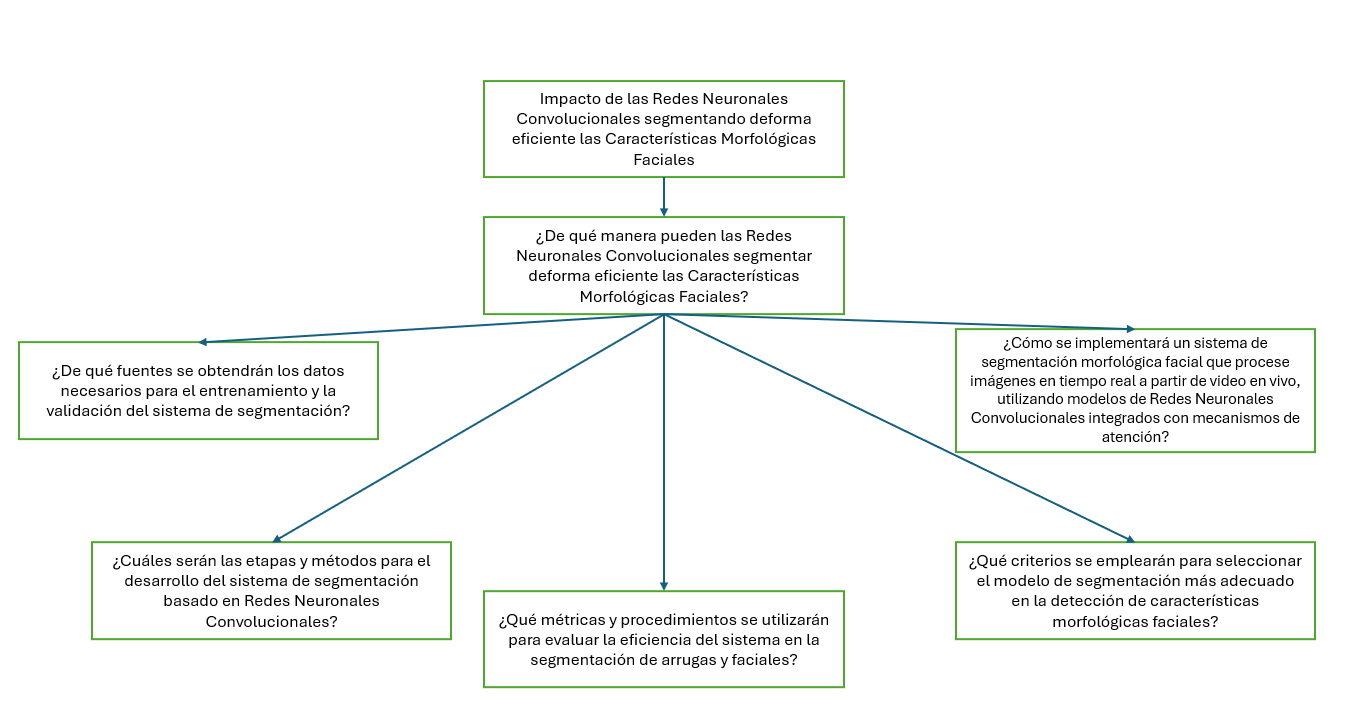
\includegraphics[width=1.00\textwidth]{anexos/arb_problemas.jpg}
			%\caption{Fuente: Elaboración propia}
		\end{center}
	\end{figure}
	\clearpage
	
	\section{Árbol de Objetivos}
	%\chapter*{Árbol de Objetivos}
	%\addcontentsline{toc}{section}{Árbol de Objetivos}
	%\renewcommand{\thechapter}{A}
	\label{anexo2}
	\begin{figure}[h]
		\begin{center}
			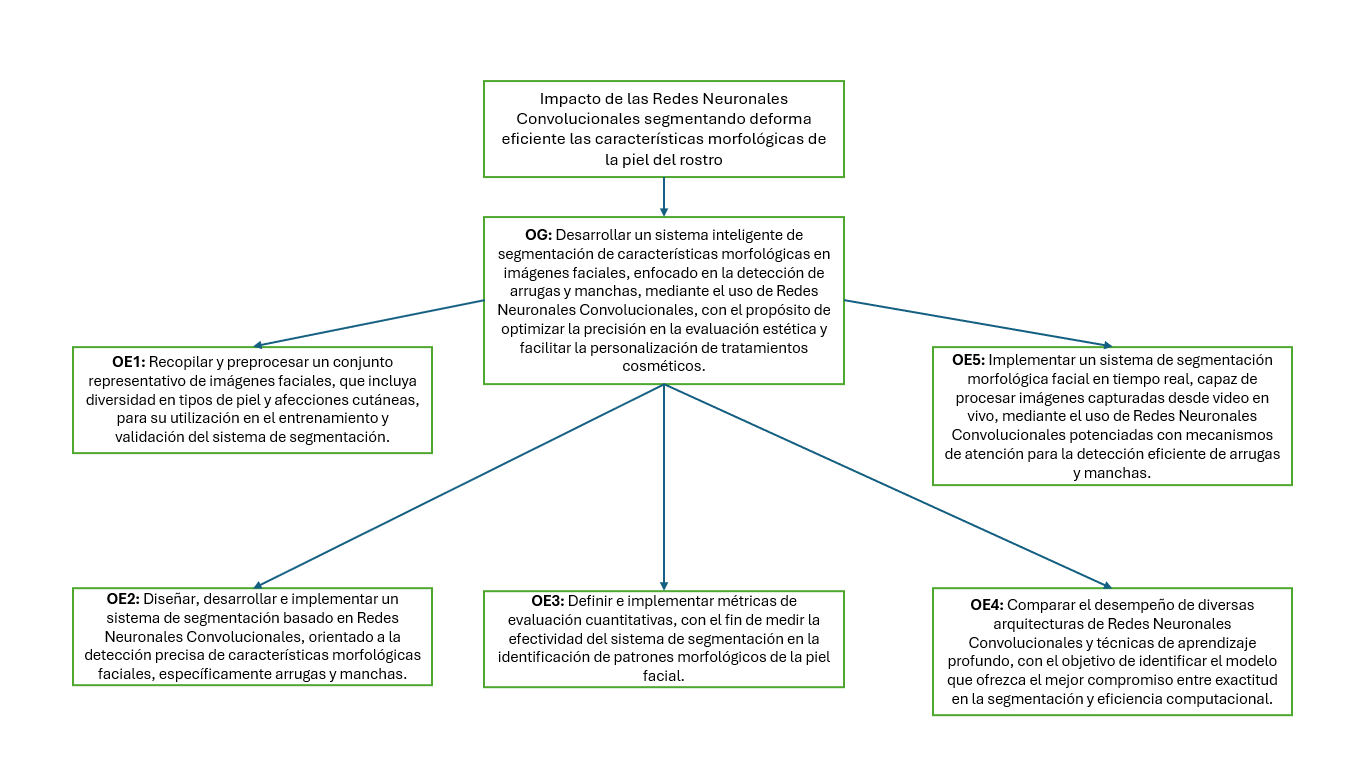
\includegraphics[width=1.00\textwidth]{anexos/arb_objetivos.jpg}
			%\caption{Fuente: Elaboración propia}
		\end{center}
	\end{figure}
	\clearpage
	
	\begin{landscape}
		\section{Matriz de Consistencia}
		\label{anexo3}
		\begin{longtable}{ p{3.5cm}p{3.5cm}p{3.5cm}p{3cm}p{3cm}p{3cm}p{3cm} }
			%\centering
			\small
			\tabularnewline \specialrule{.1em}{.05em}{.05em}
			\centering{Título de la tesis} & \multicolumn{6}{p{15cm}}{Diseño de un modelo de Deep Learning para el pre-diagnóstico de nódulos tiroideos a través de imágenes de ultrasonido}
			\tabularnewline \specialrule{.1em}{.05em}{.05em}
			\Centering{Problema General}& \Centering{Objetivo General} & \Centering{Hipótesis General} & \Centering{Variables} & \Centering{Método} \\
			\specialrule{.1em}{.05em}{.05em}
			{\ProblemaGeneral} & { \ObjetivoGeneral} & {\HipotesisGeneral} & {

				Dependiente: Pre-diagnóstico de nódulos tiroideos. Independiente: Modelo de Deep Learning.

			} \\
			\cline{1-4}
			\Centering {Problemas Específicos} & \Centering {Objetivos Específicos} & \Centering {Hipótesis Específicas} & \Centering {Variables} \\ %& \Centering {Método} \\
			\cline{1-4}
			{\Pbone} & {\Objone} & {\Hone} & {

				Dependiente: Desarrollo del modelo de Deep Learning. Independiente: Las características del conjunto de datos.

			} & \multirow{6}{3cm}{
				
				\centering Tipo de Investigación: Experimental. Alcance de la investigación: Explicativo.
			
			} \\
			\cline{1-4}
			{\Pbtwo} & {\Objtwo} & {\Htwo}  & {
				
				Dependiente: Desempeño del modelo de Deep Learning. Independiente: Técnicas de preprocesamiento.
			
			} \\ % & {aa } \\
			\cline{1-4}
			{\Pbthree} & {\Objthree} & {\Hthree}  & { 
				
				Dependiente: Comparación de modelos en la tarea de clasificación de imágenes de ultrasonido. Independiente: Las métricas de evaluación de rendimiento.
				
			} \\ % & {aa } \\
			\cline{1-4}
			{\Pbfour} & {\Objfour} & {\Hfour}  & { 
				
				Dependiente: Desempeño en la clasificación de imágenes de ultrasonido. Independiente: Las arquitecturas de Deep Learning.
			
			} \\ % & { aa} \\
			\specialrule{.1em}{.05em}{.05em}
		\end{longtable}
	\end{landscape}
	\clearpage
	
\end{document}